
\documentclass{beamer}

\usetheme{default}
\usepackage{tikz}
\usetikzlibrary{arrows,shapes.arrows,positioning,shapes}
\usepackage{graphicx}
\usepackage{hyperref}
\newcommand\red[1]{{\color{red}#1}}
\newcommand\bred[1]{{\color{red}\textbf{#1}}}
\newcommand\blue[1]{{\color{blue}#1}}
\newcommand\bblue[1]{{\color{blue}\textbf{#1}}}
\newcommand\green[1]{{\color{olive}#1}}
\newcommand\bgreen[1]{{\color{olive}\textbf{#1}}}
\newcommand\black[1]{{\color{black}#1}}
\newcommand\white[1]{{\color{white}#1}}
\newcommand\E{\text{E}}
\newcommand\V{\text{V}}
\renewcommand\P{\text{P}}
\definecolor{seagreen4}{RGB}{46, 139, 87}


\setbeamertemplate{navigation symbols}{}
\setbeamertemplate{footline}[text line]{%
\parbox{\linewidth}{\vspace*{-8pt}Ian Lundberg (UCLA)}}

\newcommand{\indep}{{\bot\negthickspace\negthickspace\bot}}

\newcommand{\goalsframe}{\begin{frame}{Learning goals for today}
By the end of class, you will be able to
\begin{itemize}
    \item understand sample splitting: a common data science procedure for choosing among many candidate estimators
 \end{itemize} 
  \vskip .2in
\end{frame}}

\title{}

\author{}

%\pgfdeclareimage[height=1cm]{university-logo}{ff_logo.jpg}
%\logo{\pgfuseimage{university-logo}}

%%%%%%%%%%%%%%%%%%%%%%%%%%%%%%
\begin{document}

%\begin{frame}
%  \titlepage
%\end{frame}

\begin{frame}
\begin{tikzpicture}[x = \textwidth, y = \textheight]
\node at (0,0) {};
\node at (1,1) {};
\node[anchor = north west, align = left, font = \huge] at (0,.9) {Social\\Data\\Science};
\node[anchor = north east, align = right] (number) at (1,.9) {Soc 114\\Winter 2025};
\node[anchor = north, font = \Large, align = center] at (.5,.5) {Data-Driven Selection of an Estimator};
\end{tikzpicture}
\end{frame}


\begin{frame}{Plan for today}
These slides are in two parts:
\begin{itemize}
\item slides from a concrete research project of mine
\item generalizing that project to a data science idea: sample splitting to select an estimator
\end{itemize}
\end{frame}


\begin{frame}

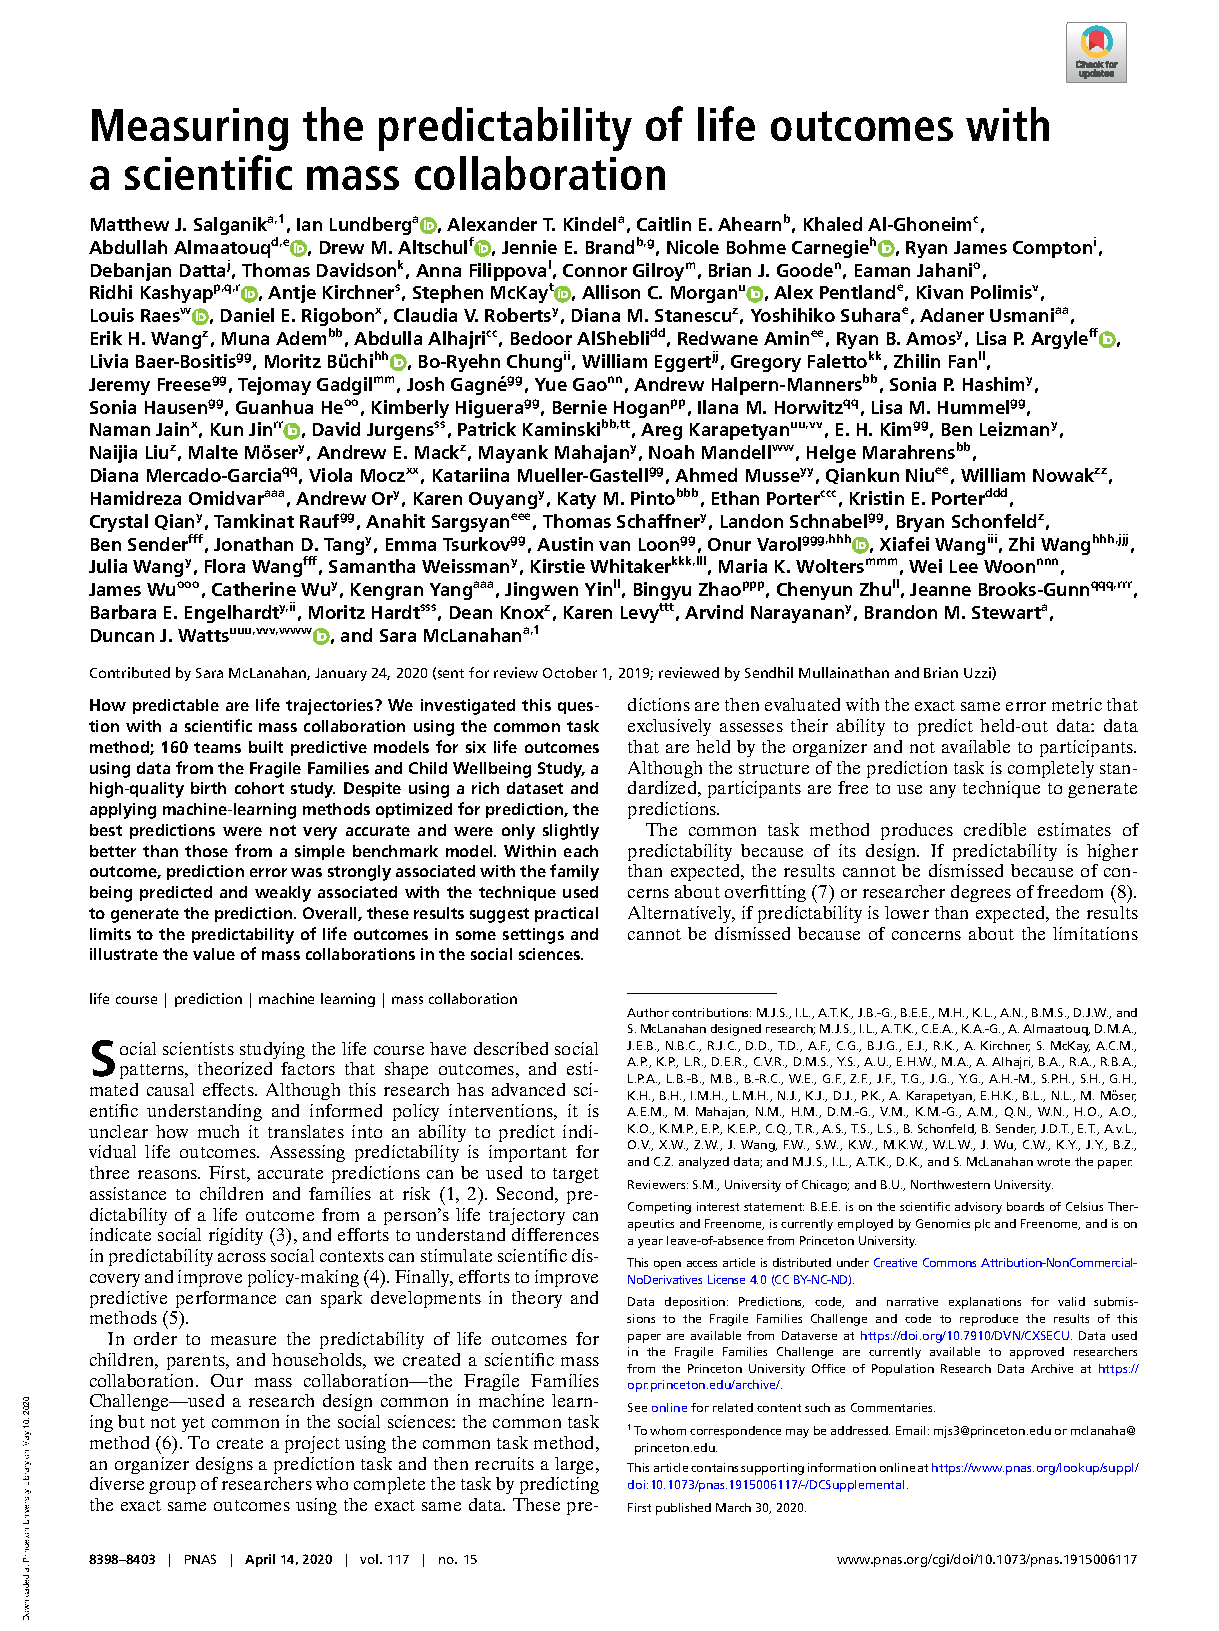
\includegraphics[width = \textwidth, trim = {0 6.5in 0 .6in}, clip]{figures/pnas_page1}

\end{frame}

%%%%%%%%%%%%%%%%%%%%%%%%%%
\begin{frame}

\begin{center}

\includegraphics[width=0.8\textwidth]{figures/wikipedia_logo}
\end{center}

\end{frame}
%%%%%%%%%%%%%%%%%%%%%%%%%%%
\begin{frame}

\begin{center}

\includegraphics[width=\textwidth]{figures/lander_initial_2001_title}
\end{center}

\end{frame}
%%%%%%%%%%%%%%%%%%%%%%%%%%
\begin{frame}

\begin{center}
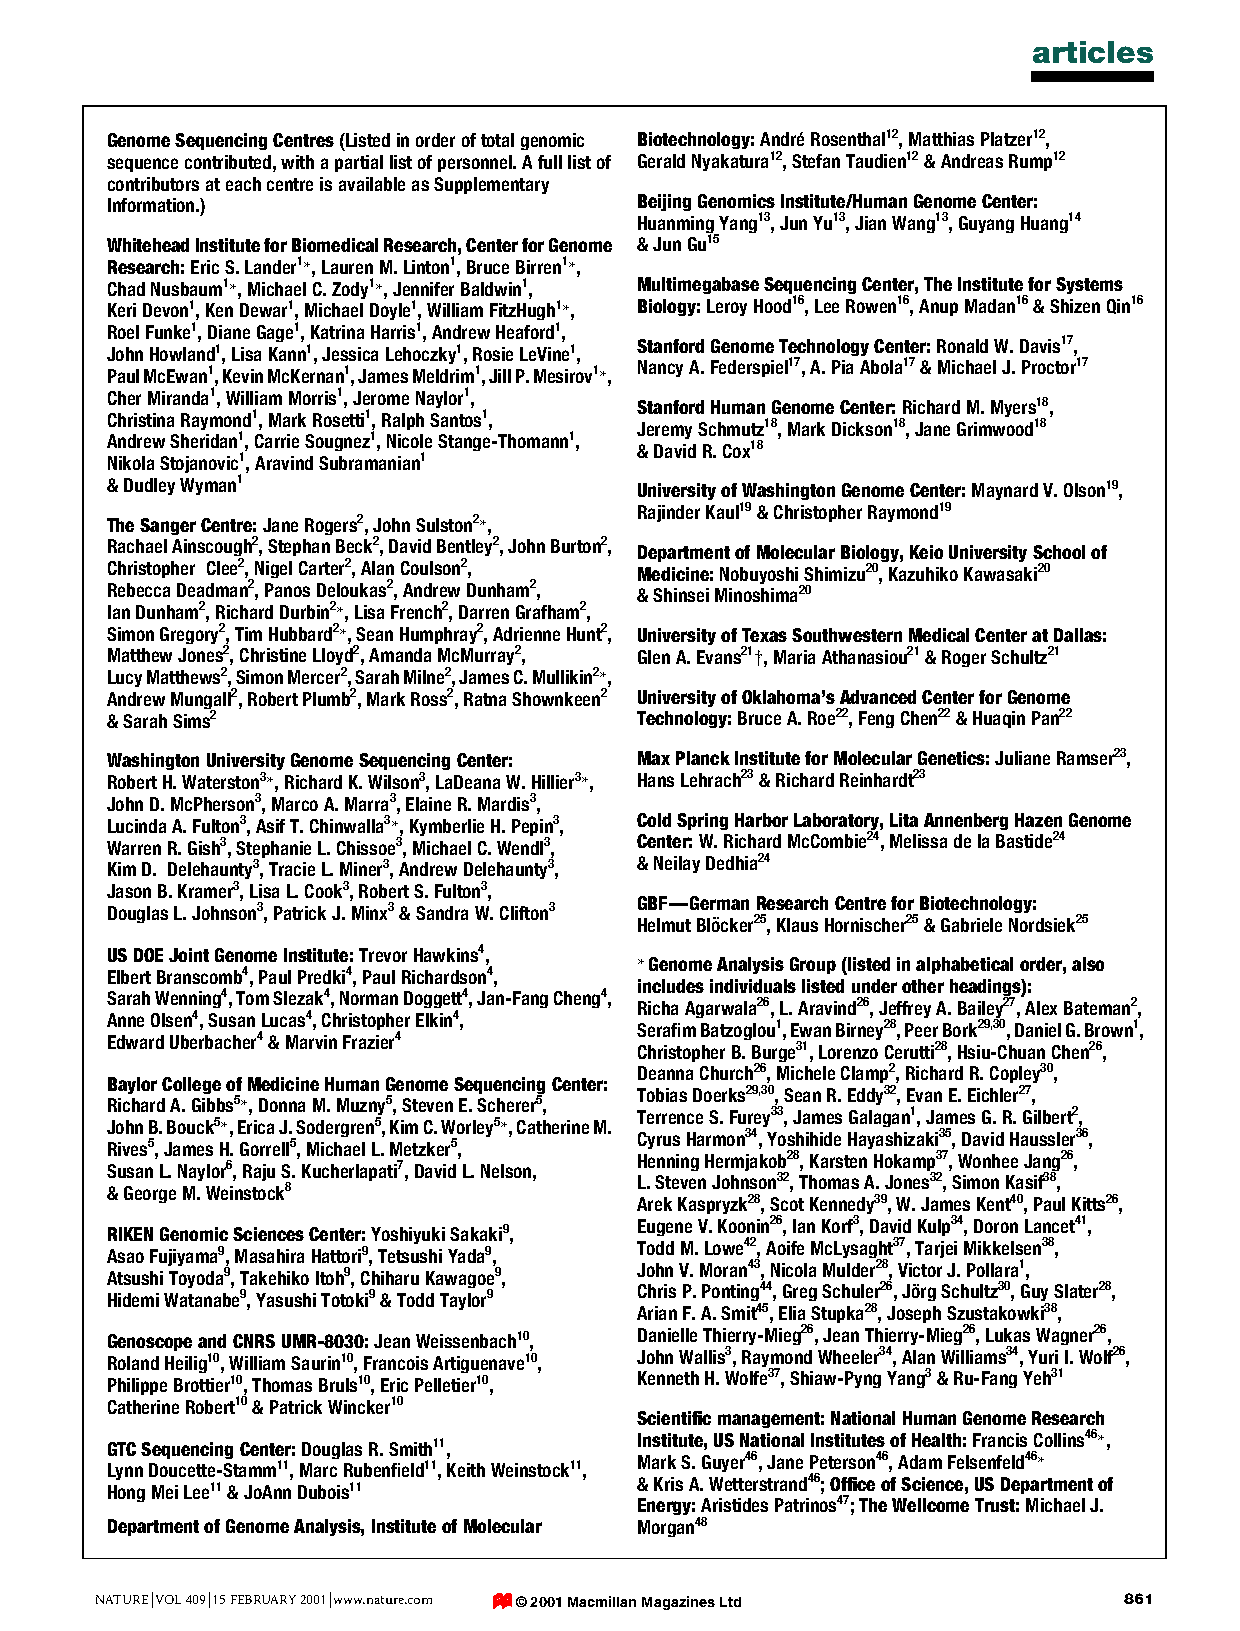
\includegraphics[height=\textheight]{figures/lander_initial_2001_authors}
\end{center}

\end{frame}
%%%%%%%%%%%%%%%%%%%%%%%%%%
\begin{frame}

\begin{center}
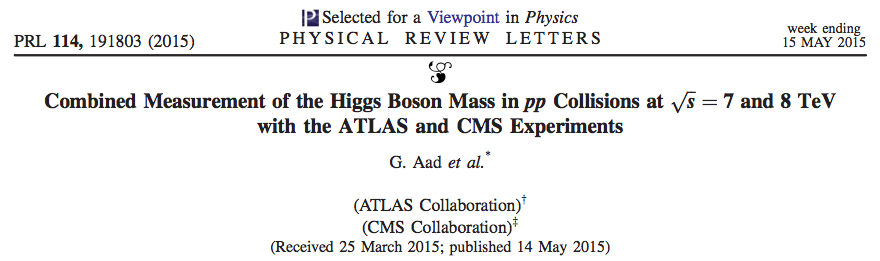
\includegraphics[width=\textwidth]{figures/aad_combined_2015_title}
\end{center}

\vfill
{\tiny \url{https://doi.org/10.1103/PhysRevLett.114.191803}}

\end{frame}
%%%%%%%%%%%%%%%%%%%%%%%%%%
\begin{frame}

\begin{center}
\only<1>{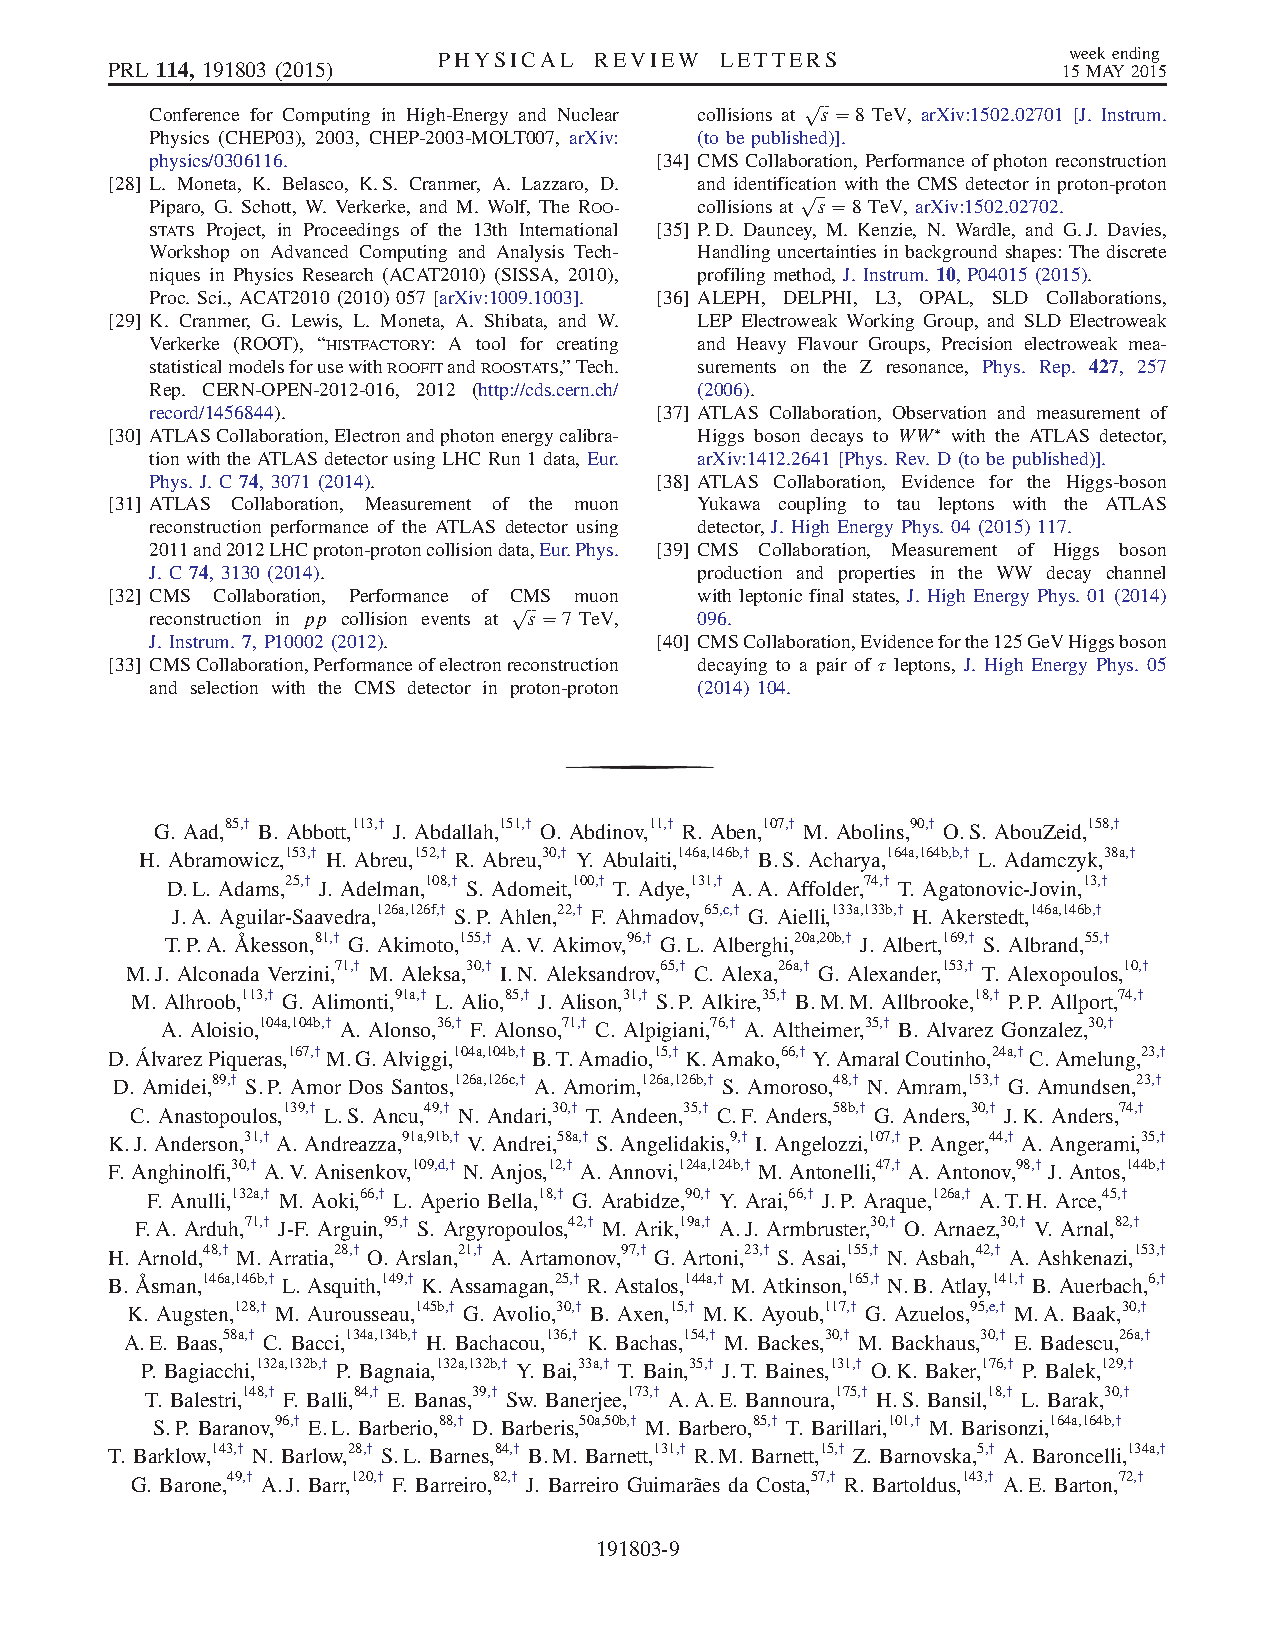
\includegraphics[height=\textheight]{figures/aad_combined_2015_authors_01}}
\only<2>{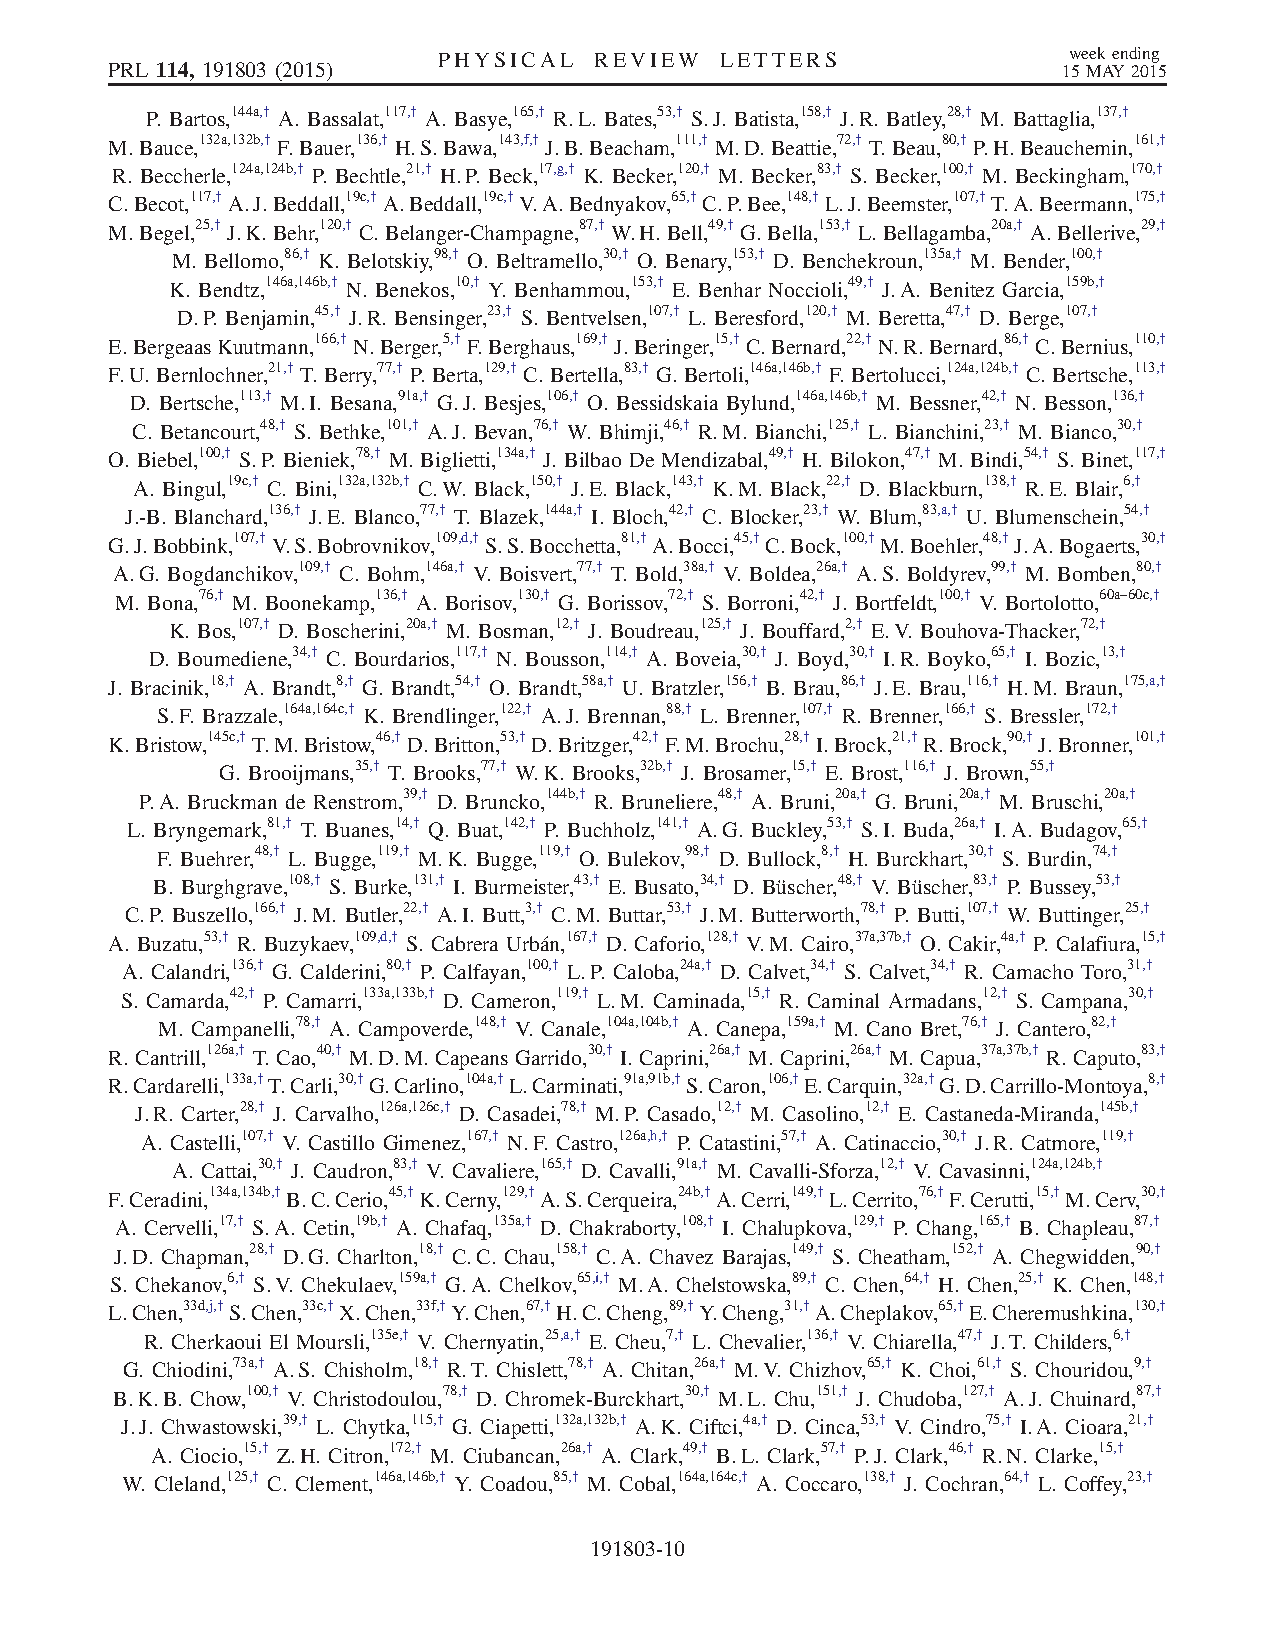
\includegraphics[height=\textheight]{figures/aad_combined_2015_authors_02}}
\only<3>{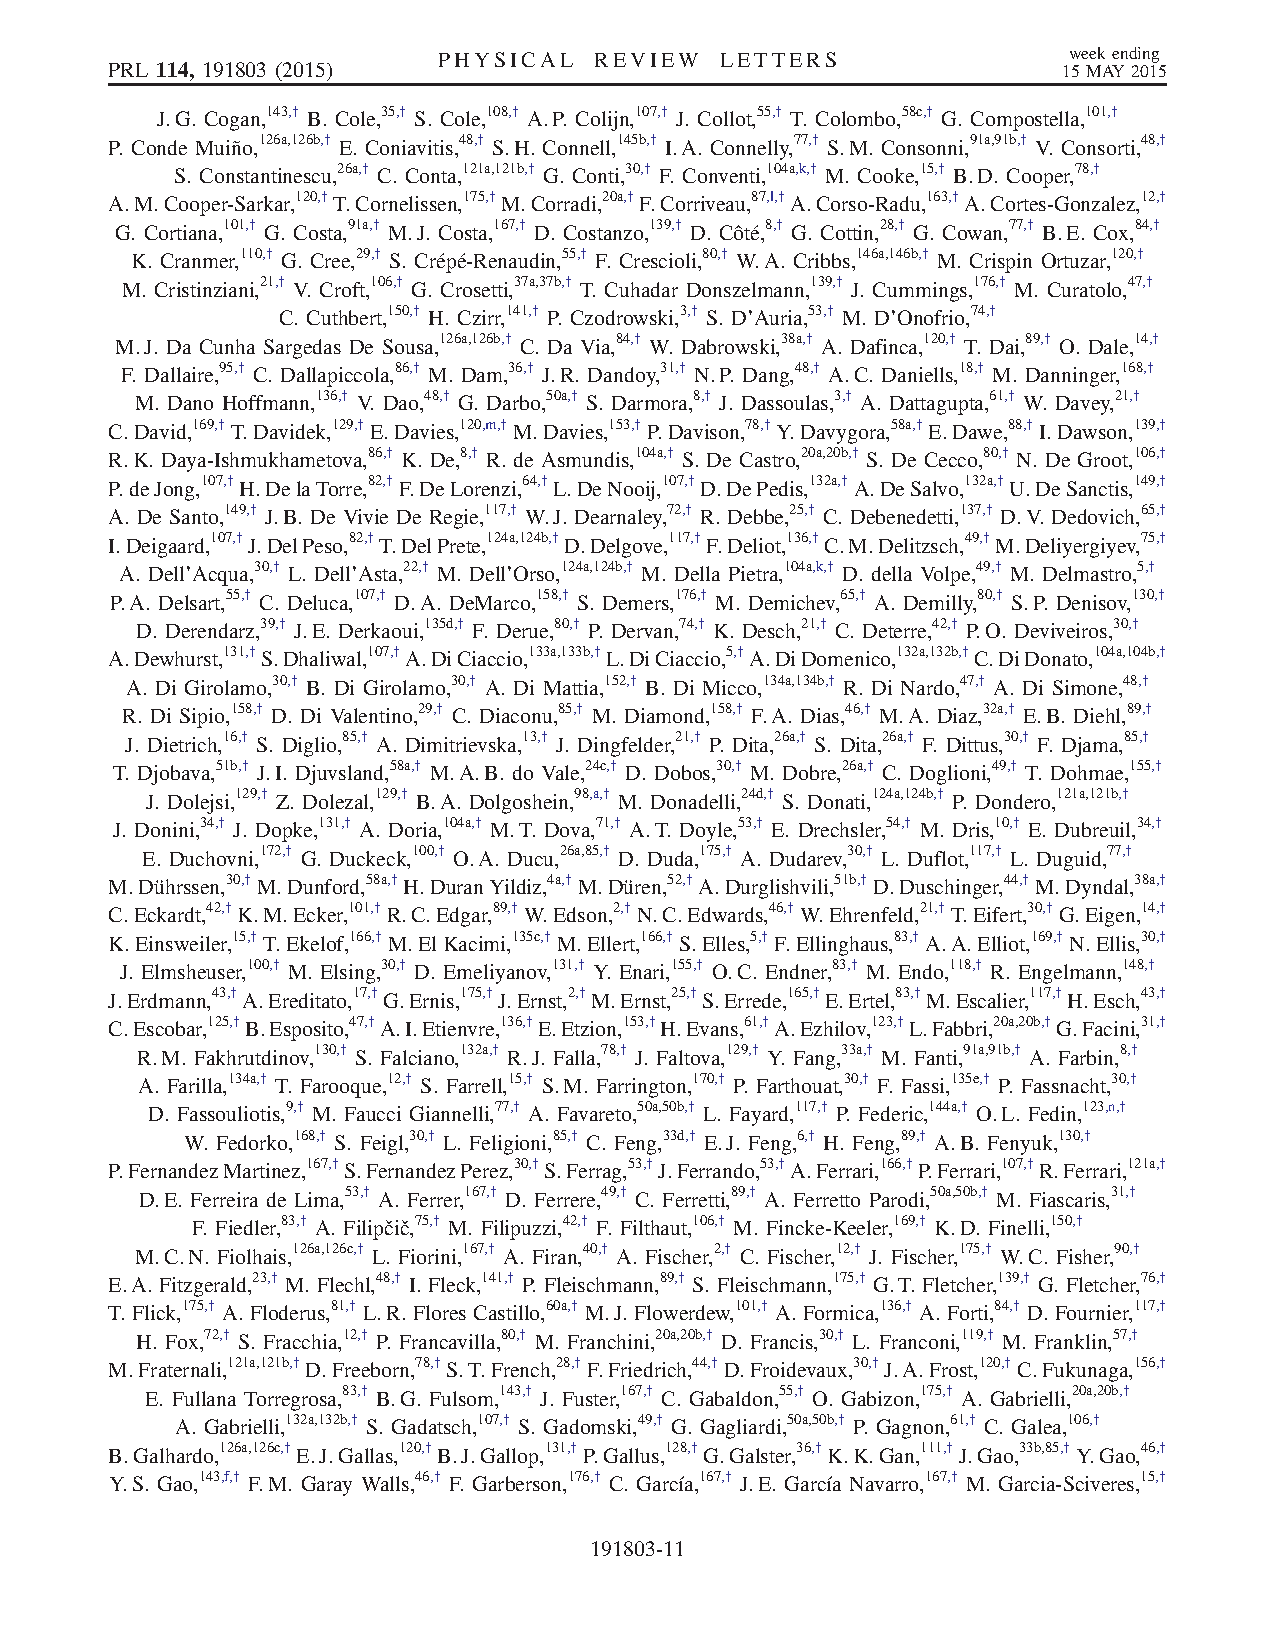
\includegraphics[height=\textheight]{figures/aad_combined_2015_authors_03}}
\only<4>{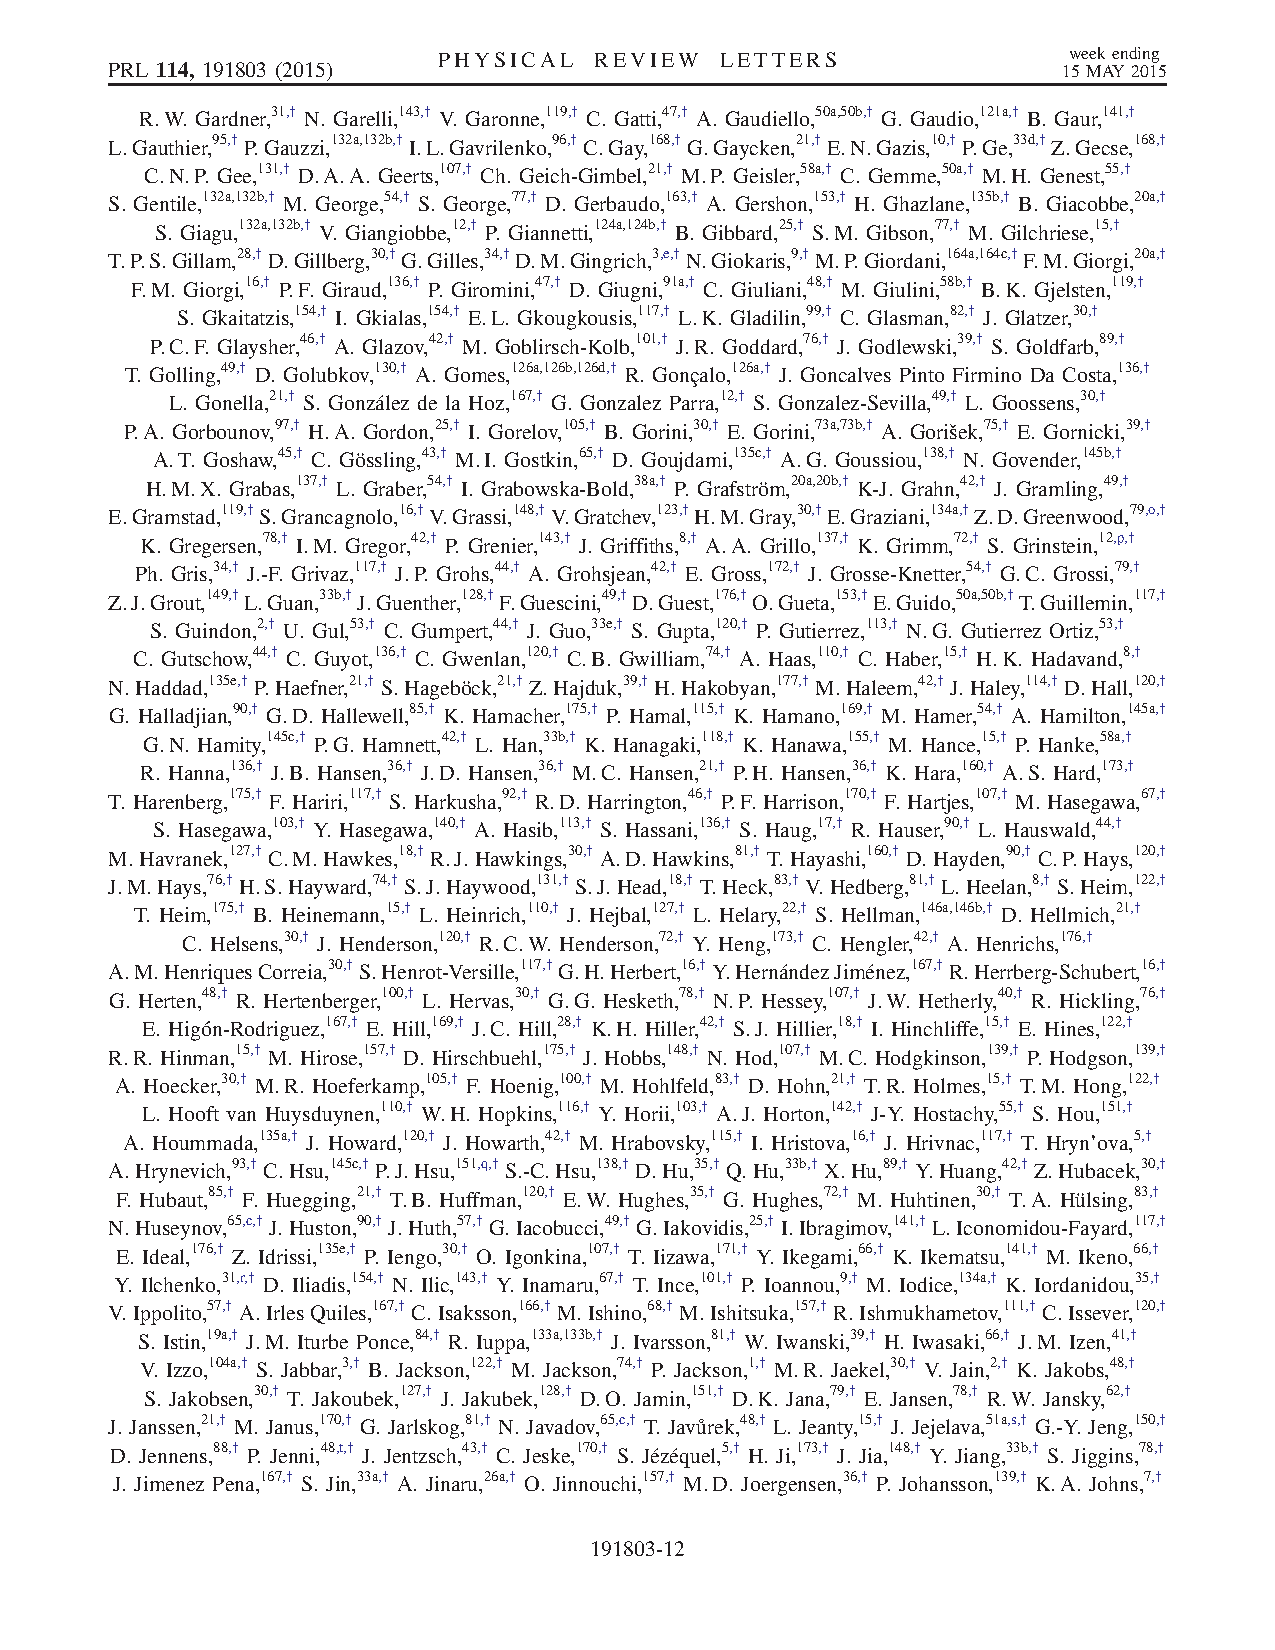
\includegraphics[height=\textheight]{figures/aad_combined_2015_authors_04}}
\only<5>{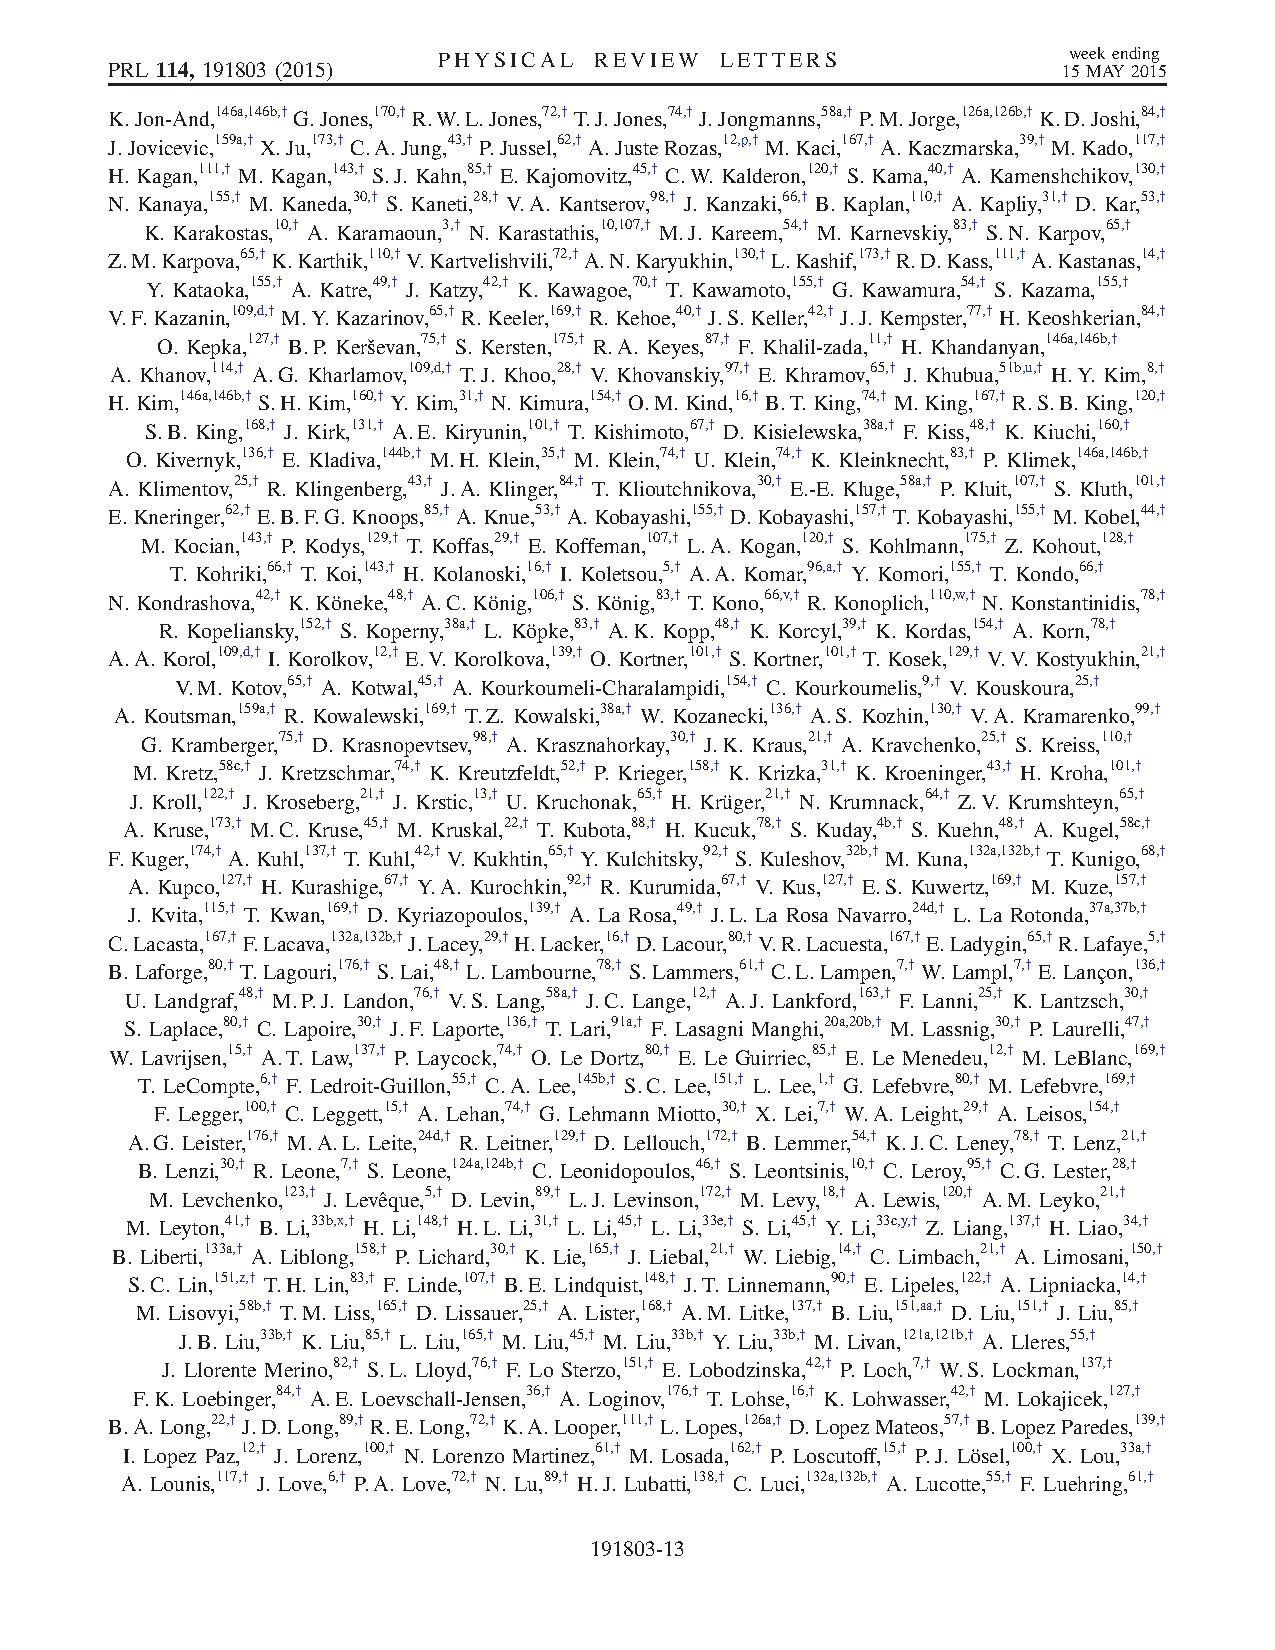
\includegraphics[height=\textheight]{figures/aad_combined_2015_authors_05}}
\only<6>{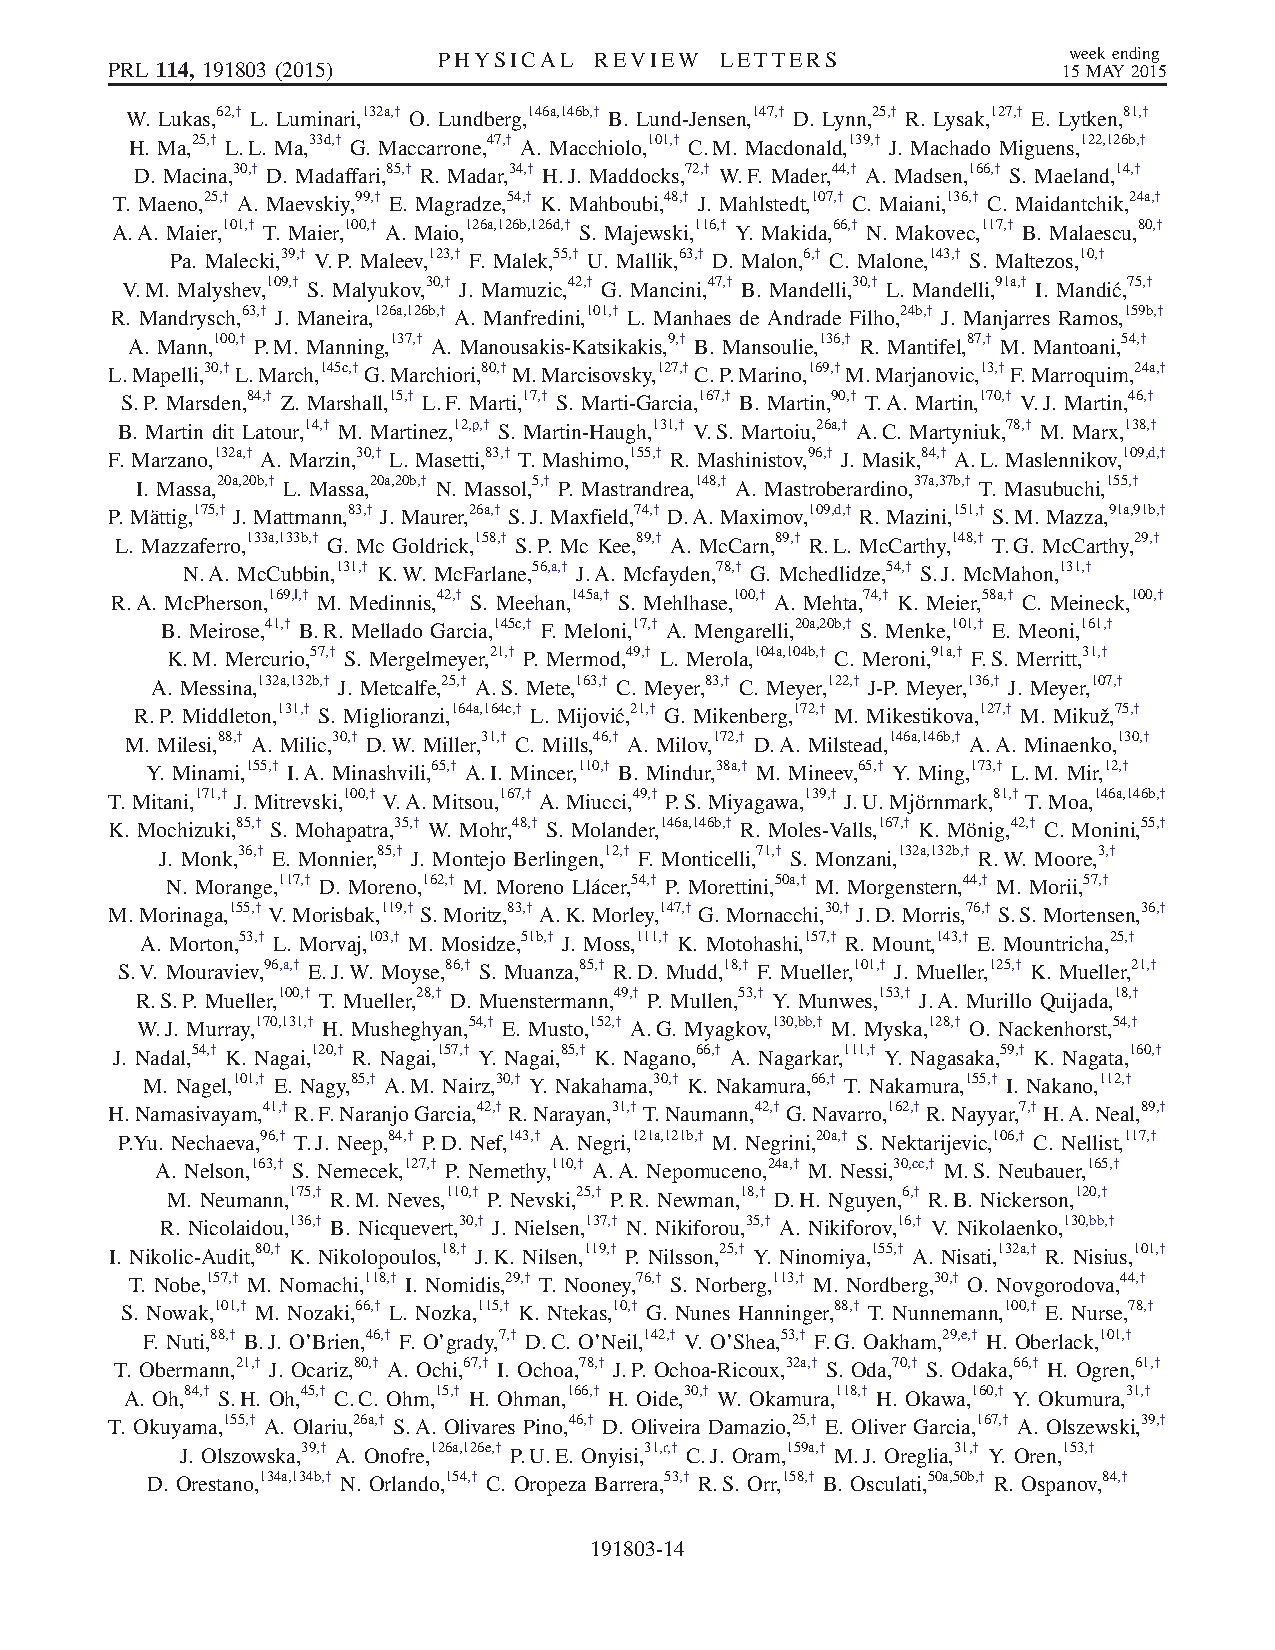
\includegraphics[height=\textheight]{figures/aad_combined_2015_authors_06}}
\only<7>{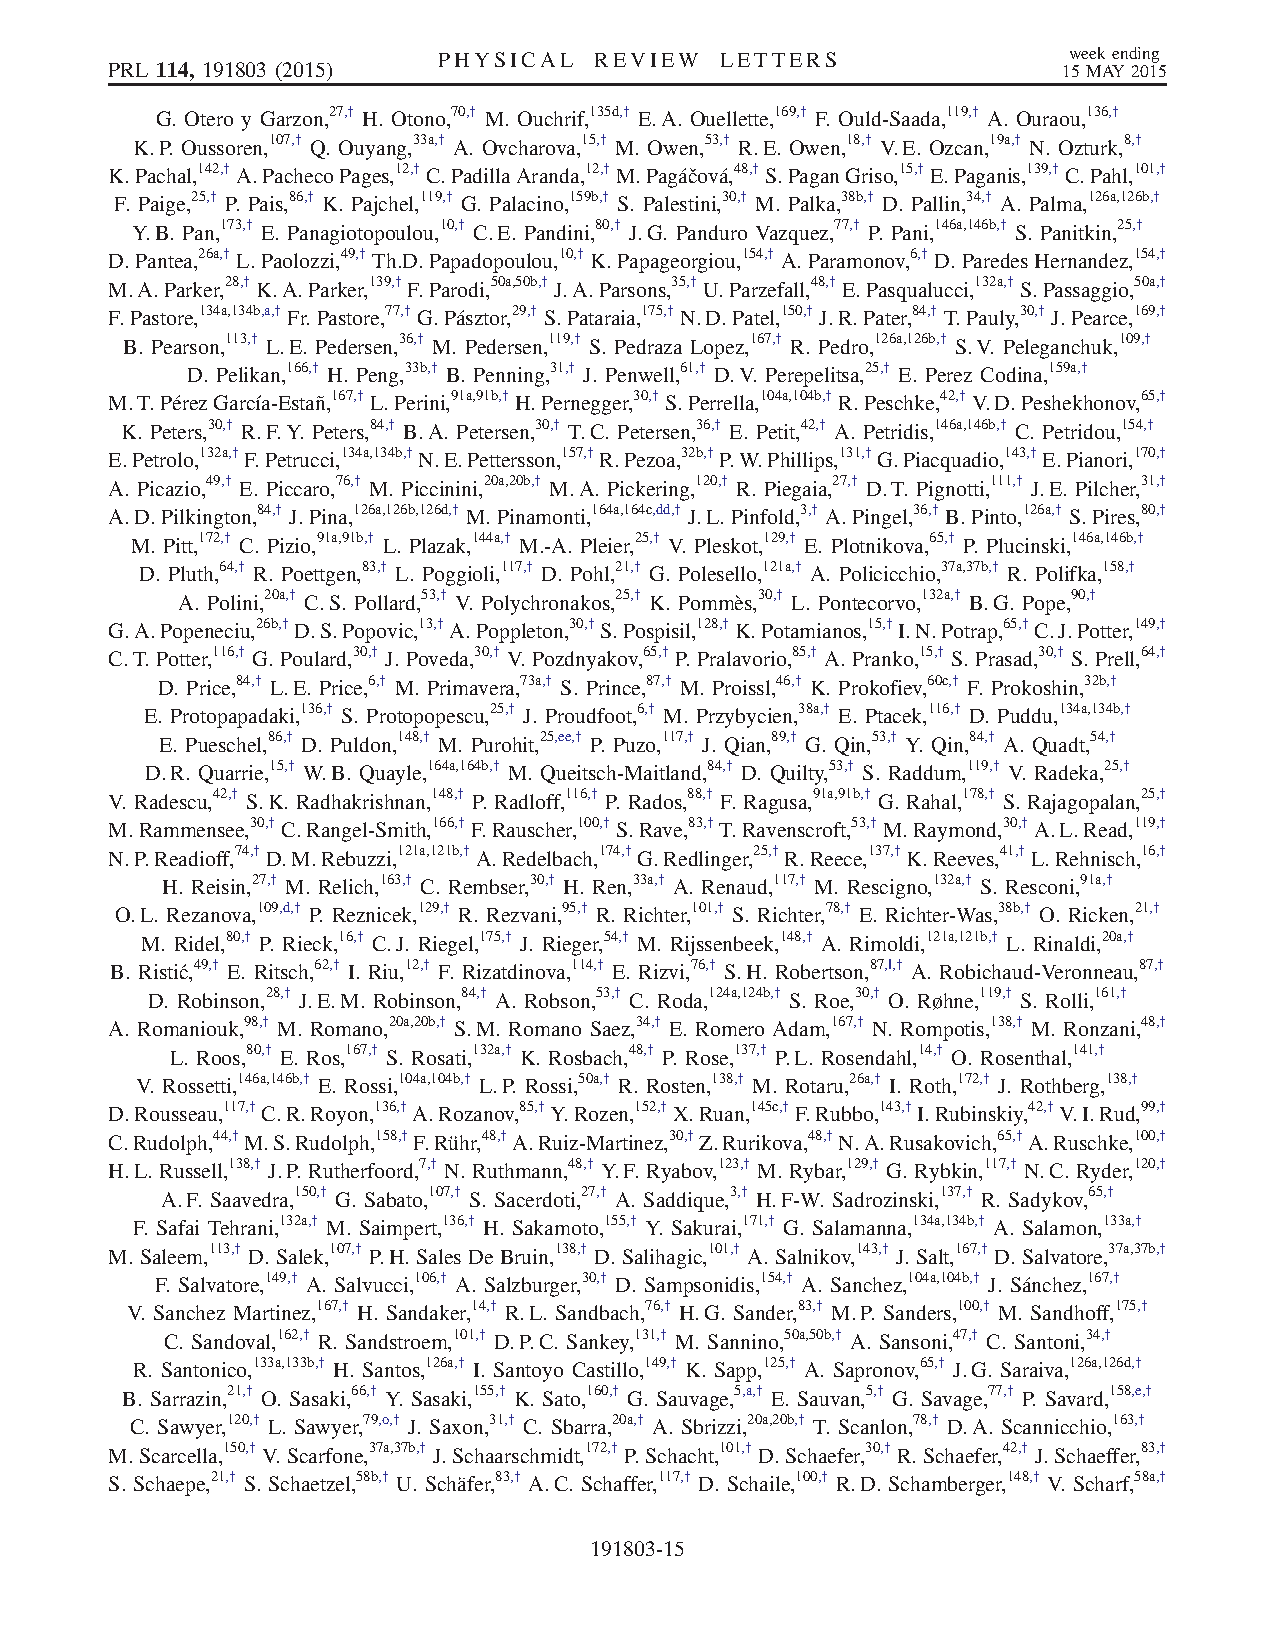
\includegraphics[height=\textheight]{figures/aad_combined_2015_authors_07}}
\only<8>{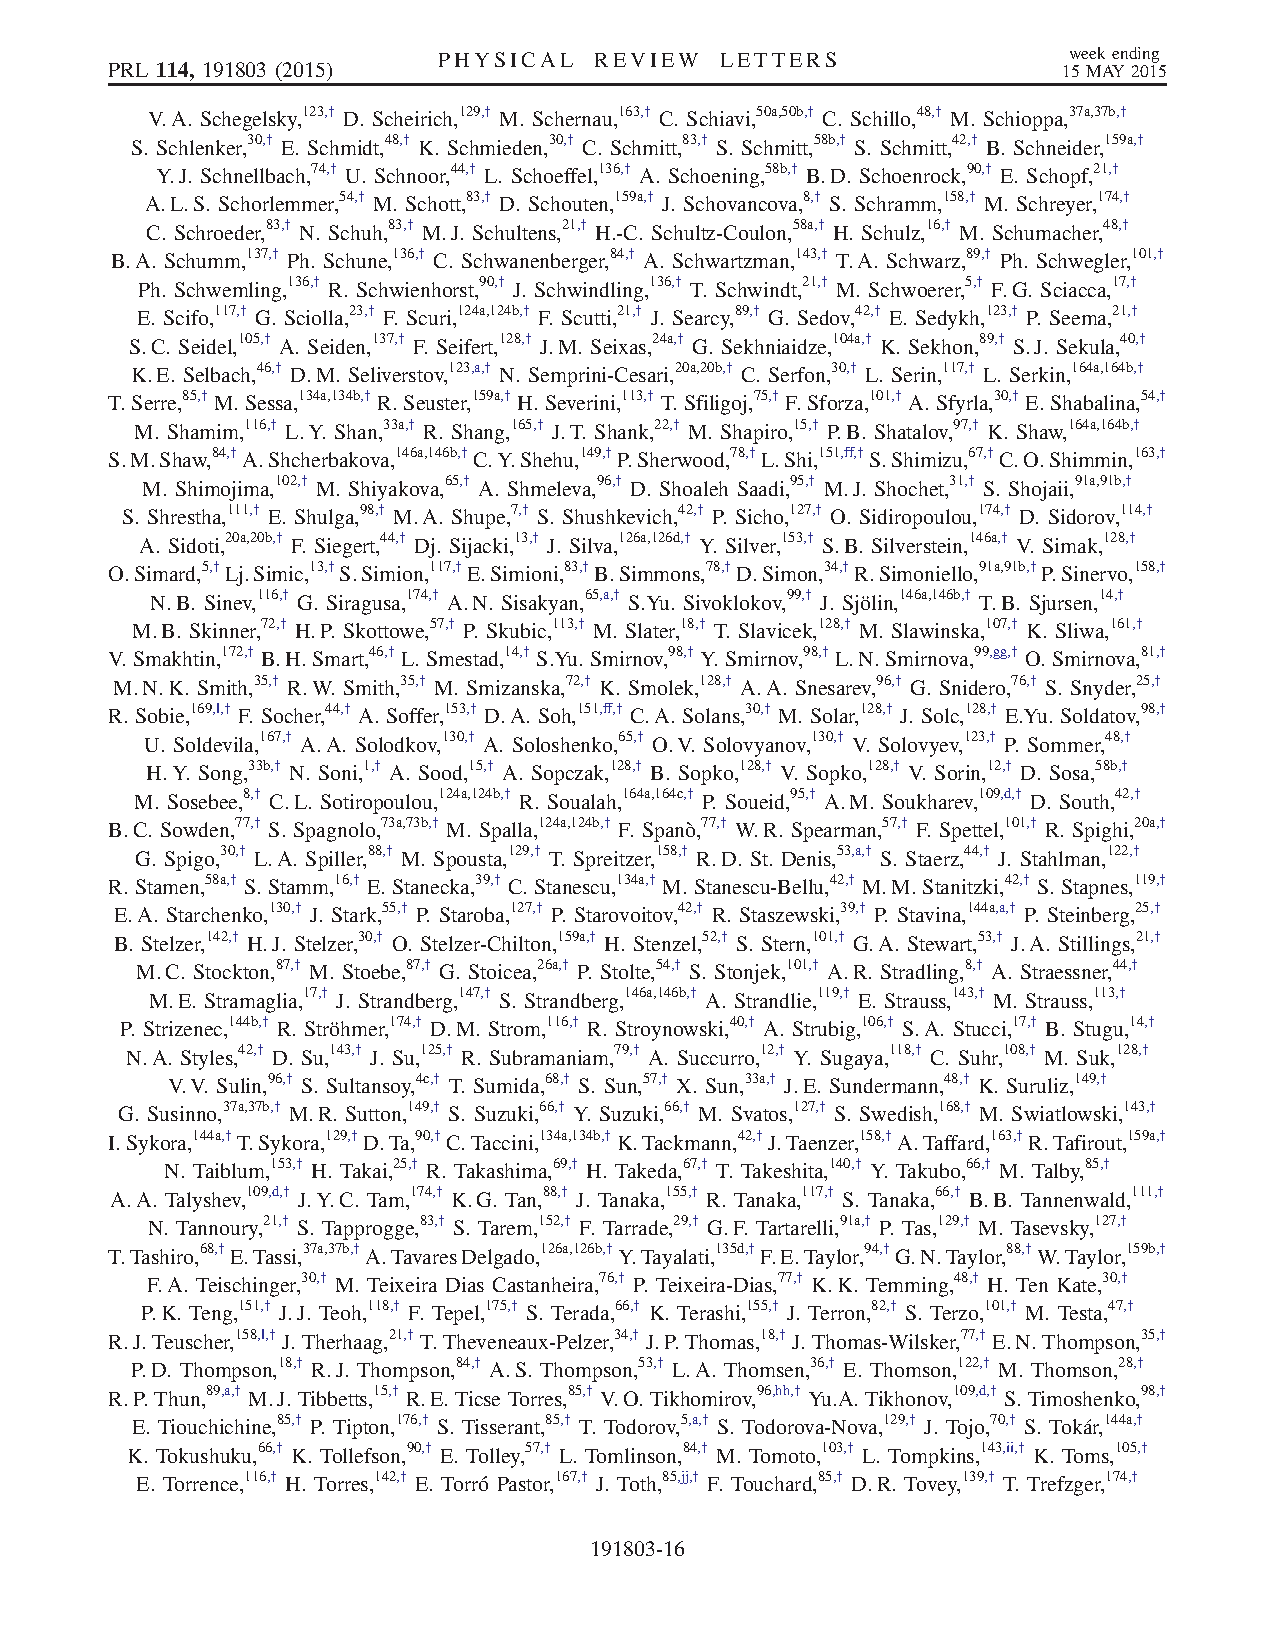
\includegraphics[height=\textheight]{figures/aad_combined_2015_authors_08}}
\only<9>{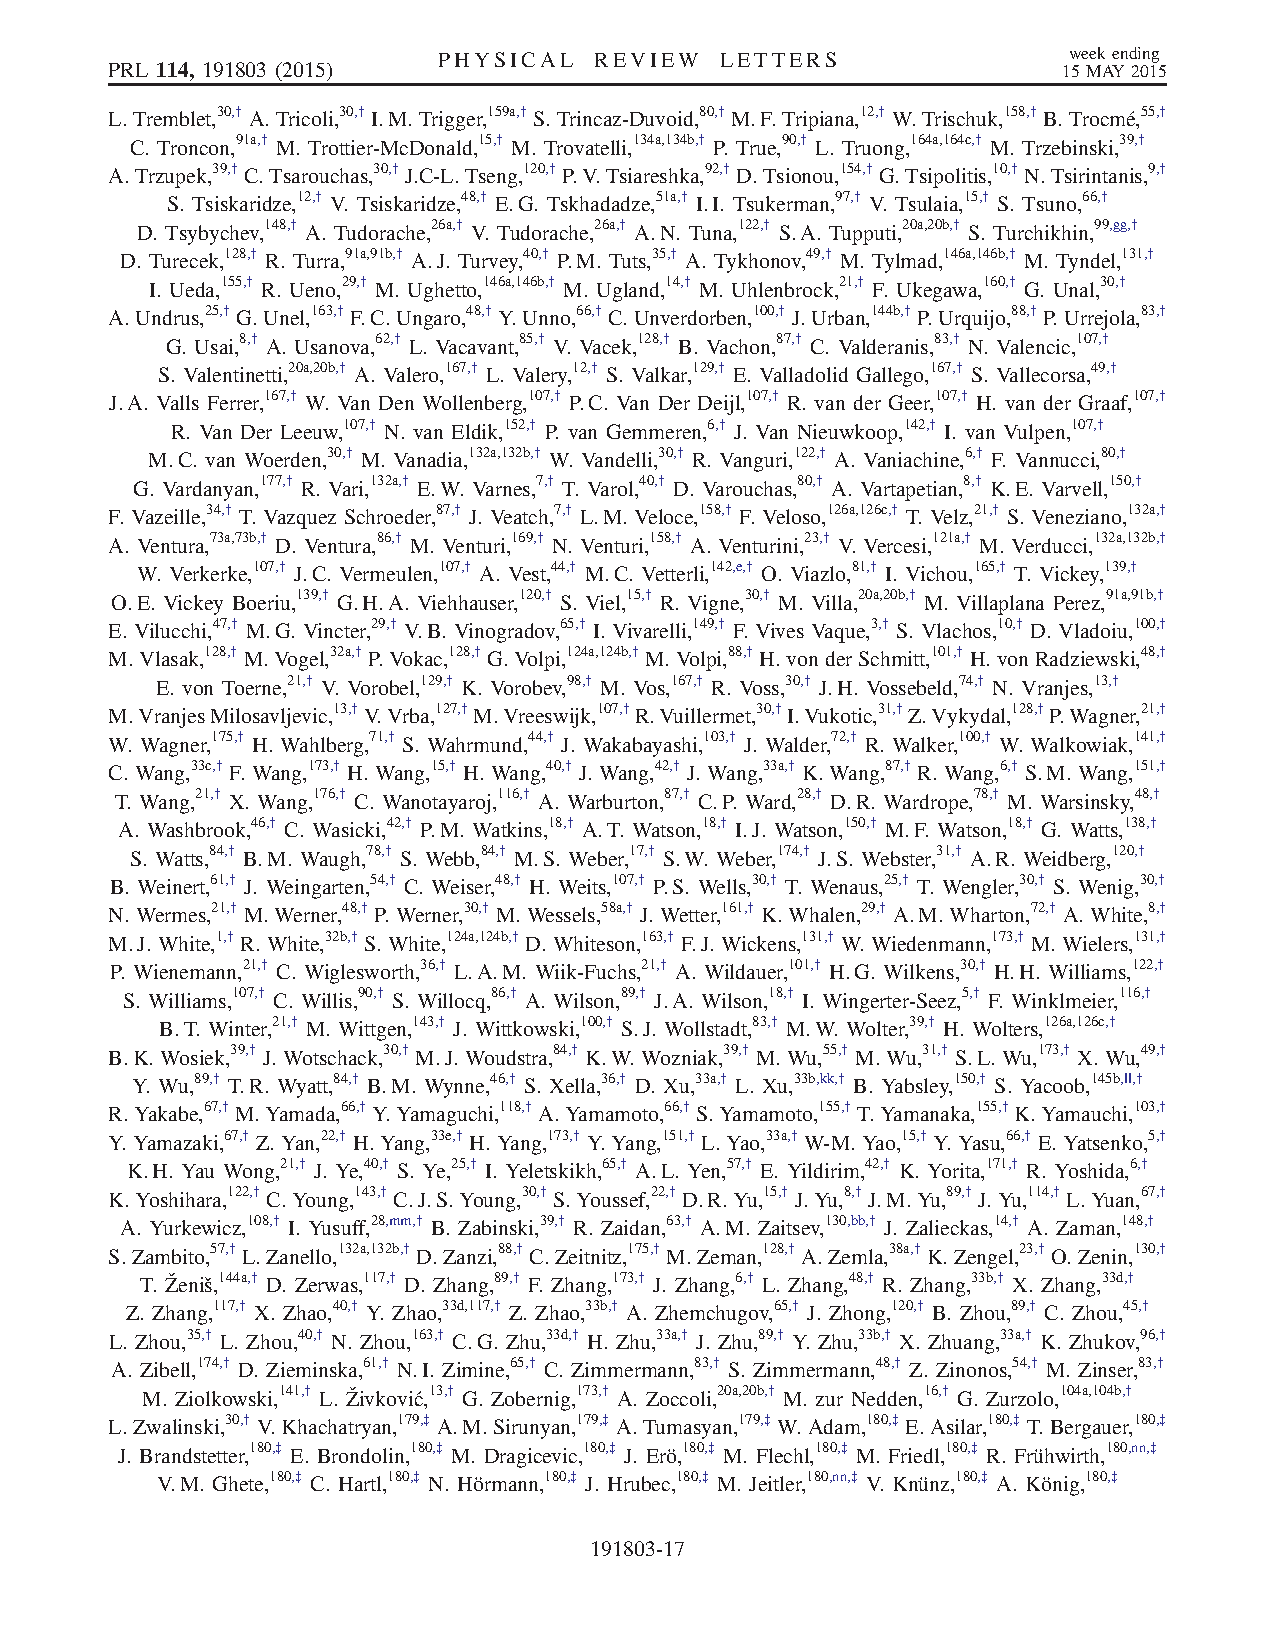
\includegraphics[height=\textheight]{figures/aad_combined_2015_authors_09}}
\only<10>{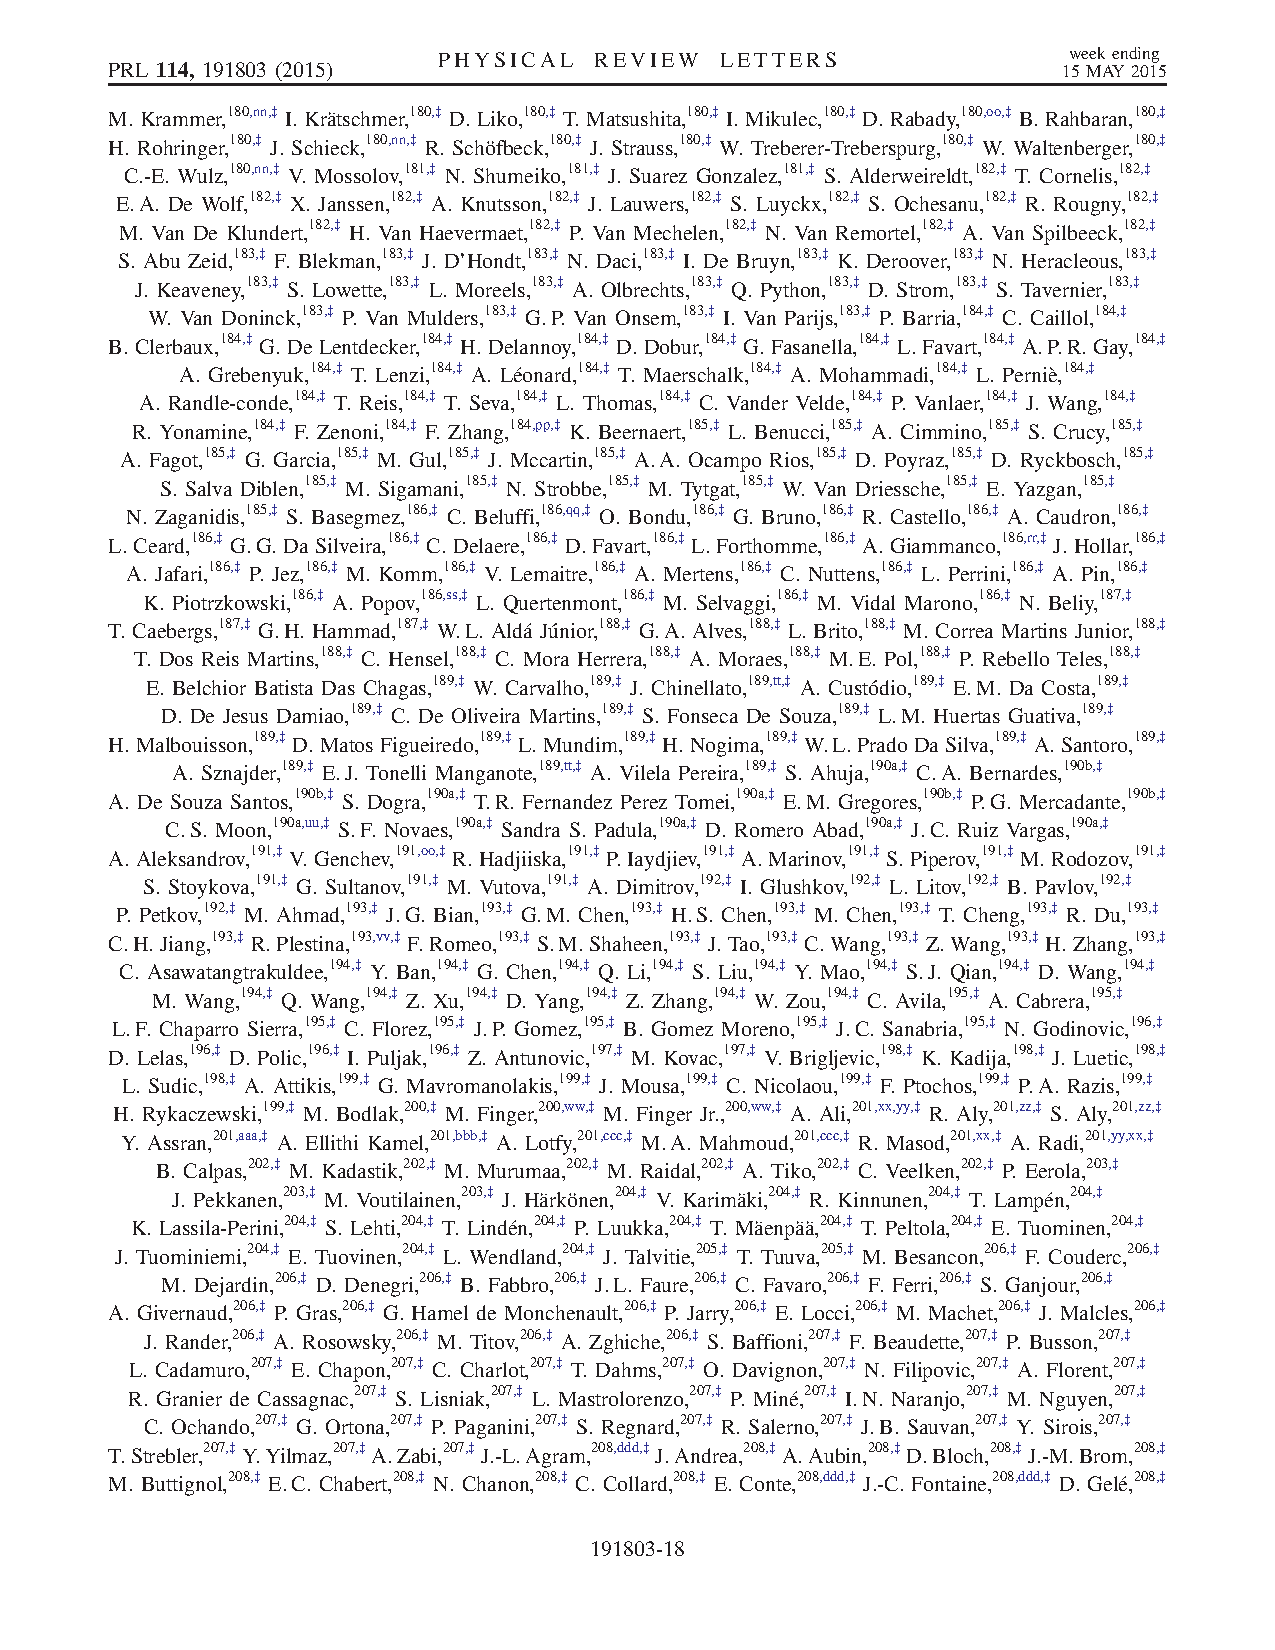
\includegraphics[height=\textheight]{figures/aad_combined_2015_authors_10}}
\only<11>{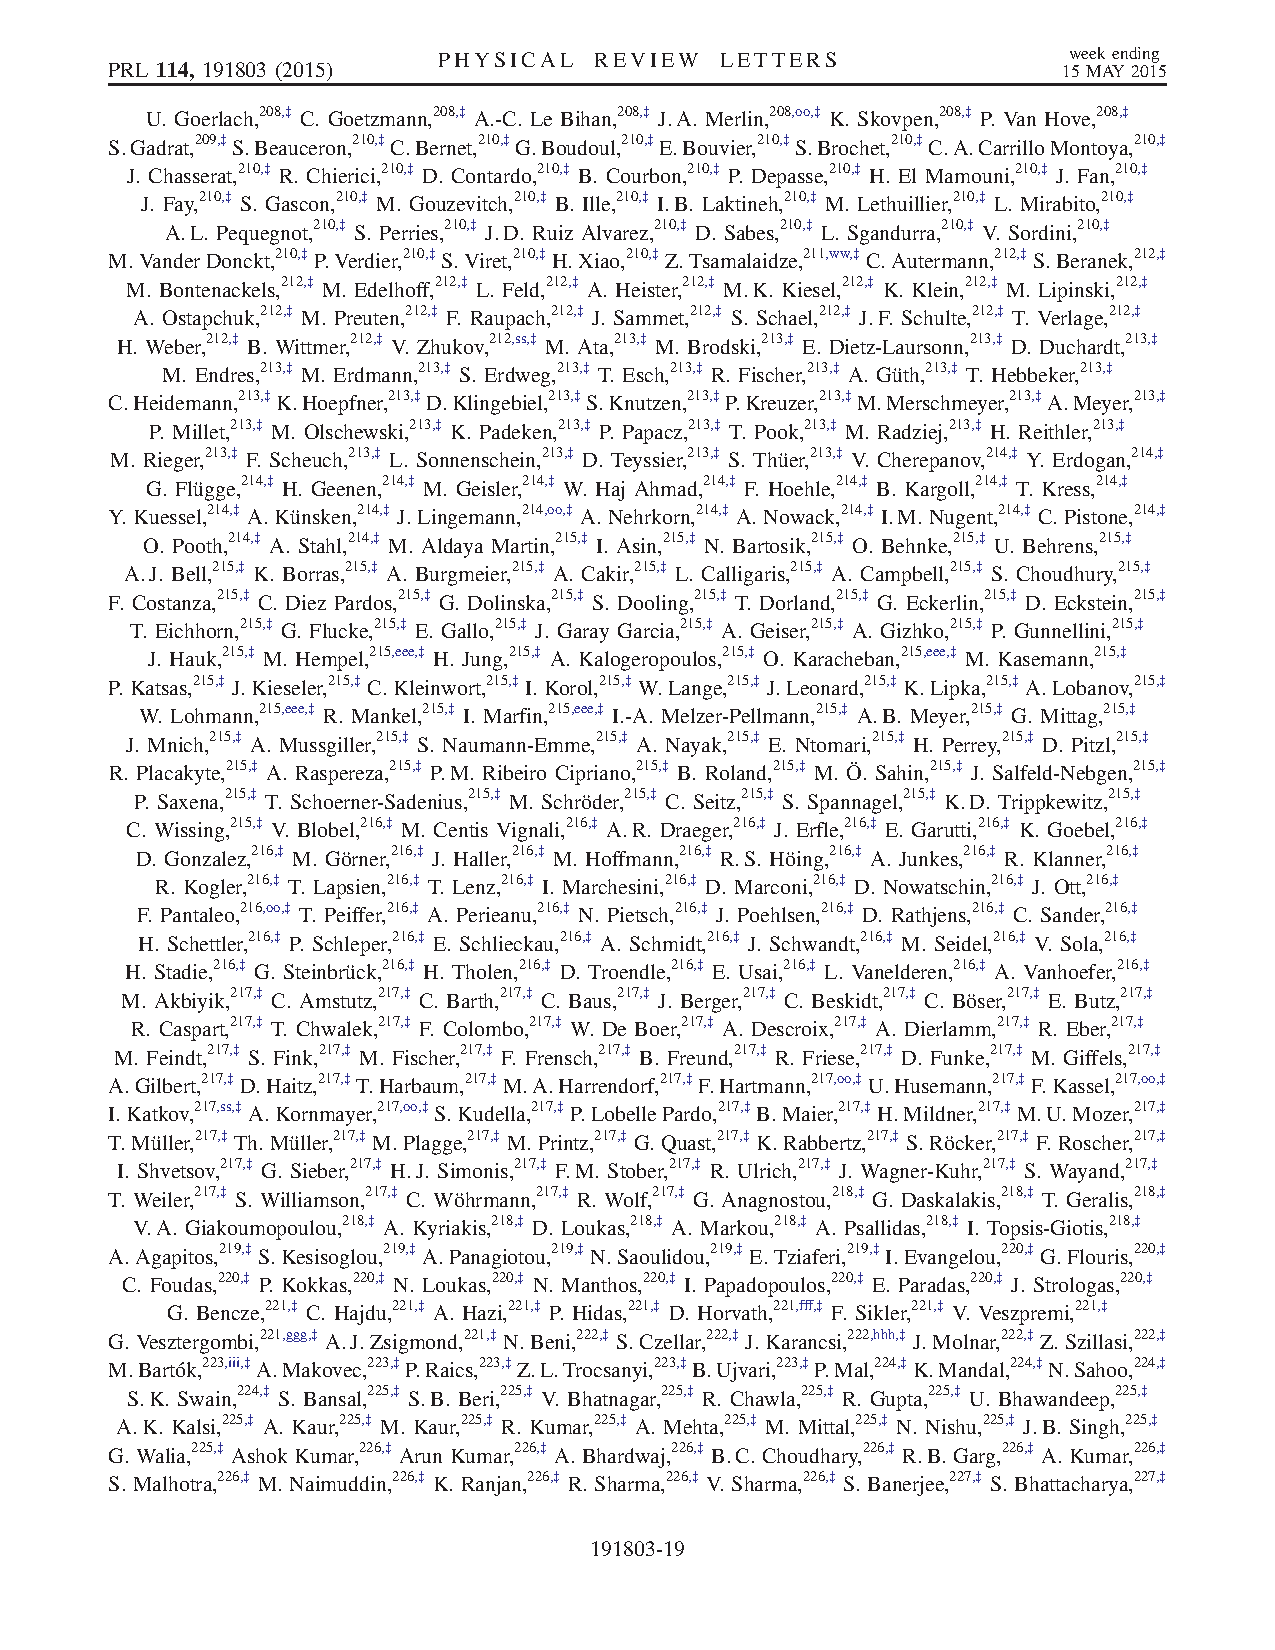
\includegraphics[height=\textheight]{figures/aad_combined_2015_authors_11}}
\only<12>{
\includegraphics[height=\textheight]{figures/aad_combined_2015_authors_12}}
\only<13>{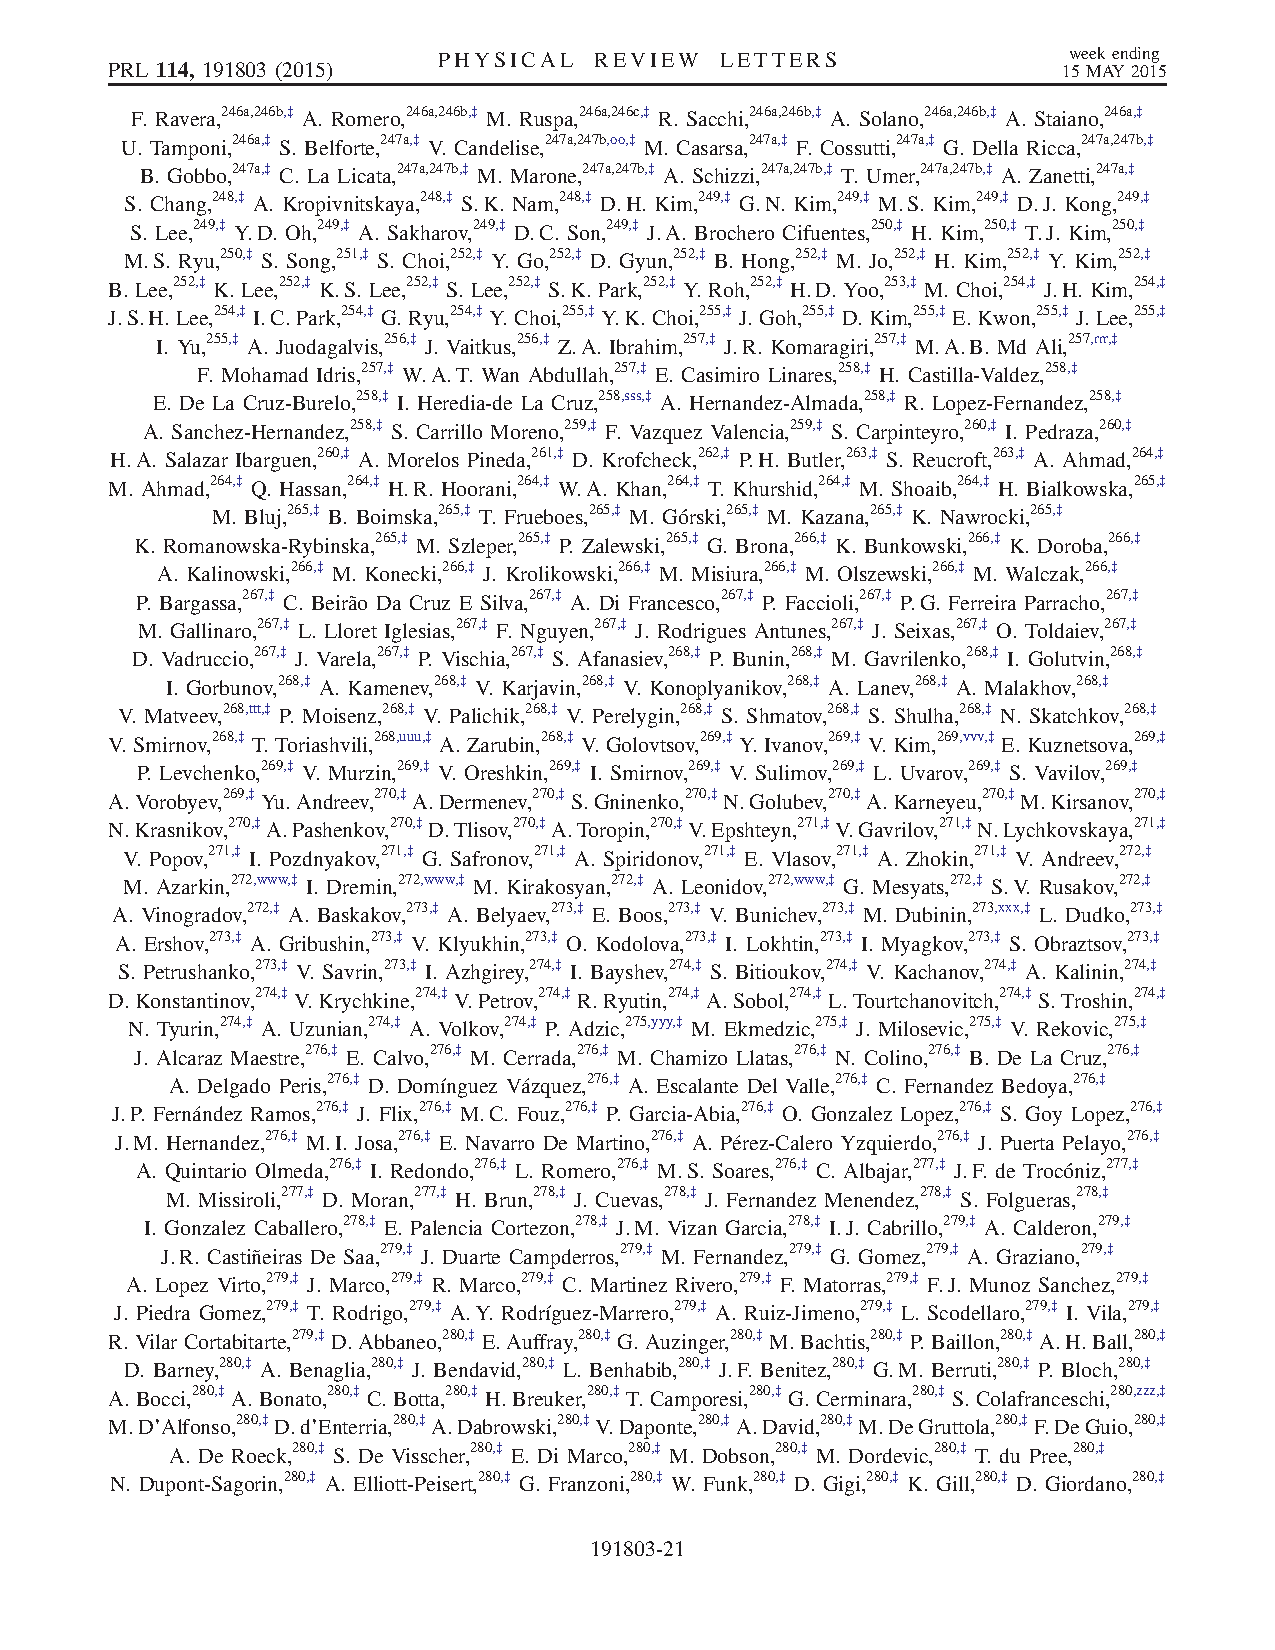
\includegraphics[height=\textheight]{figures/aad_combined_2015_authors_13}}
\only<14>{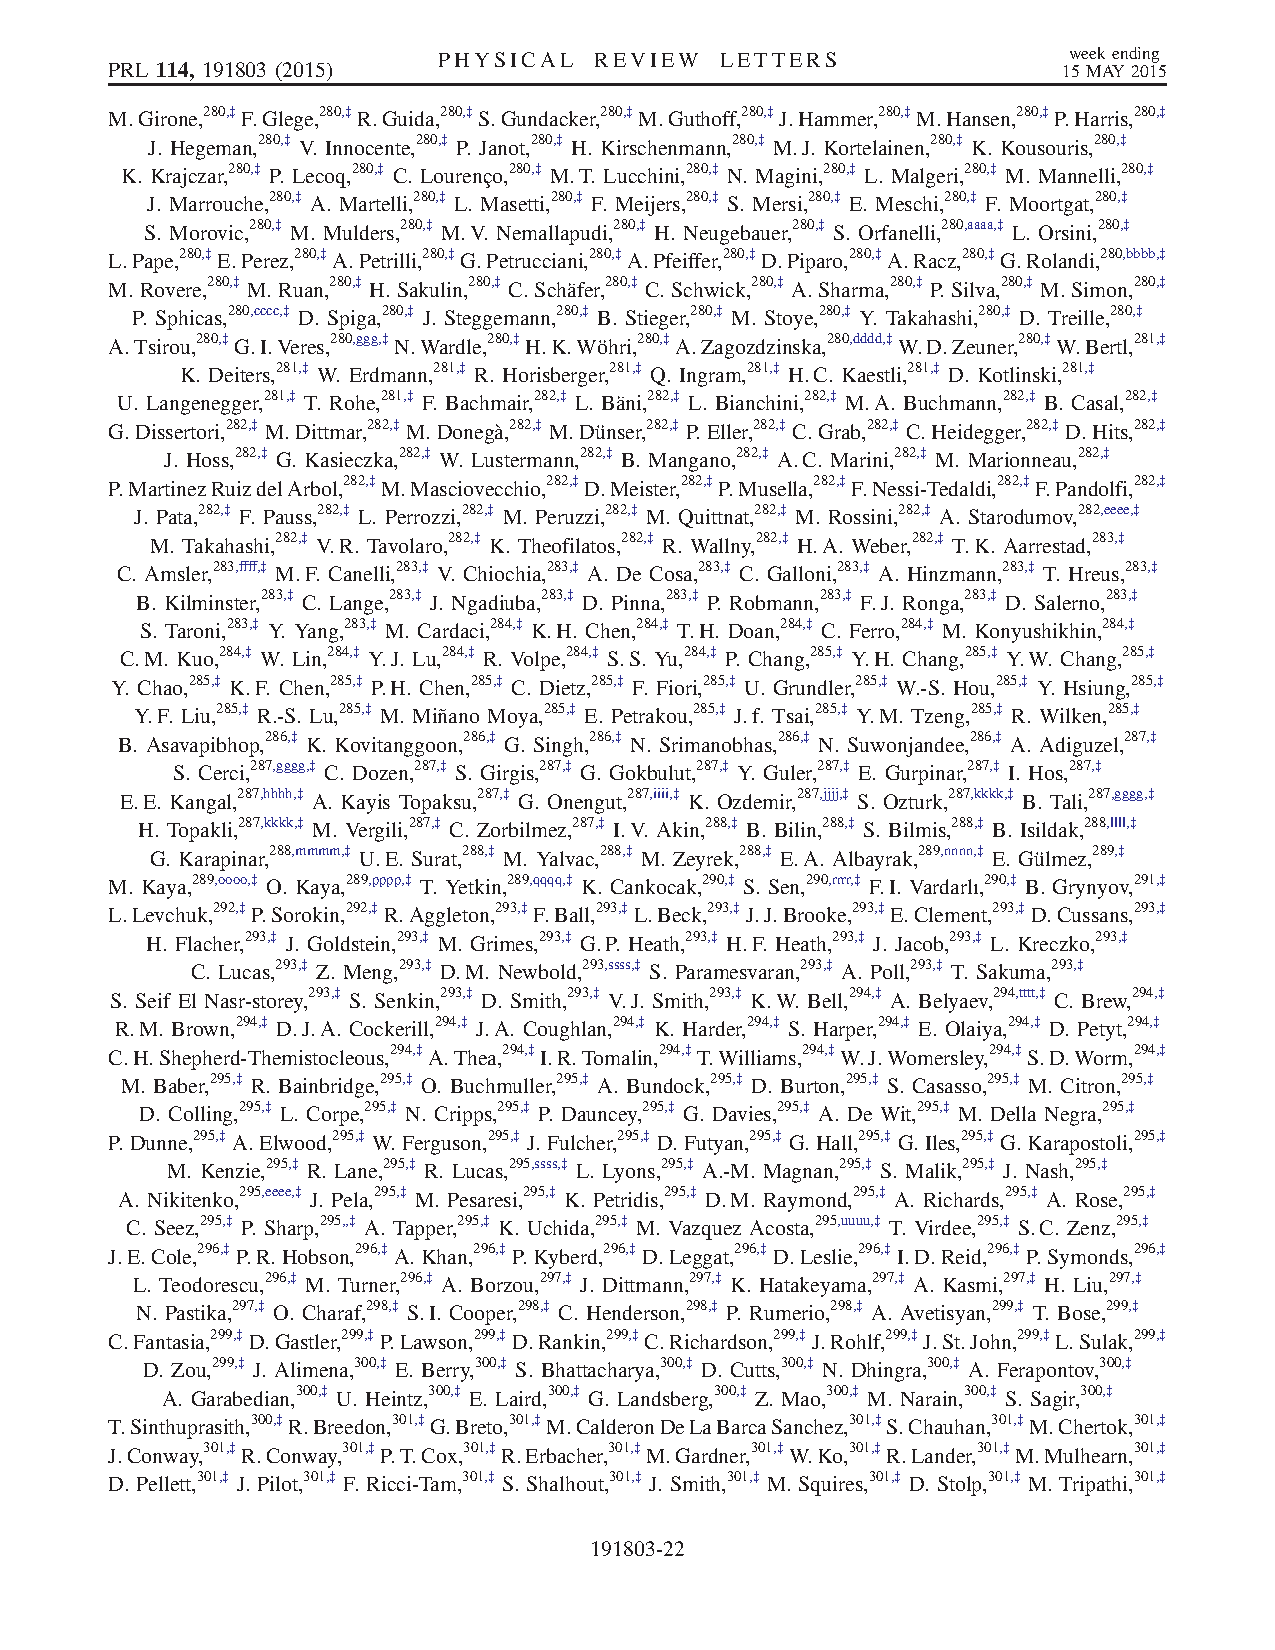
\includegraphics[height=\textheight]{figures/aad_combined_2015_authors_14}}
\only<15>{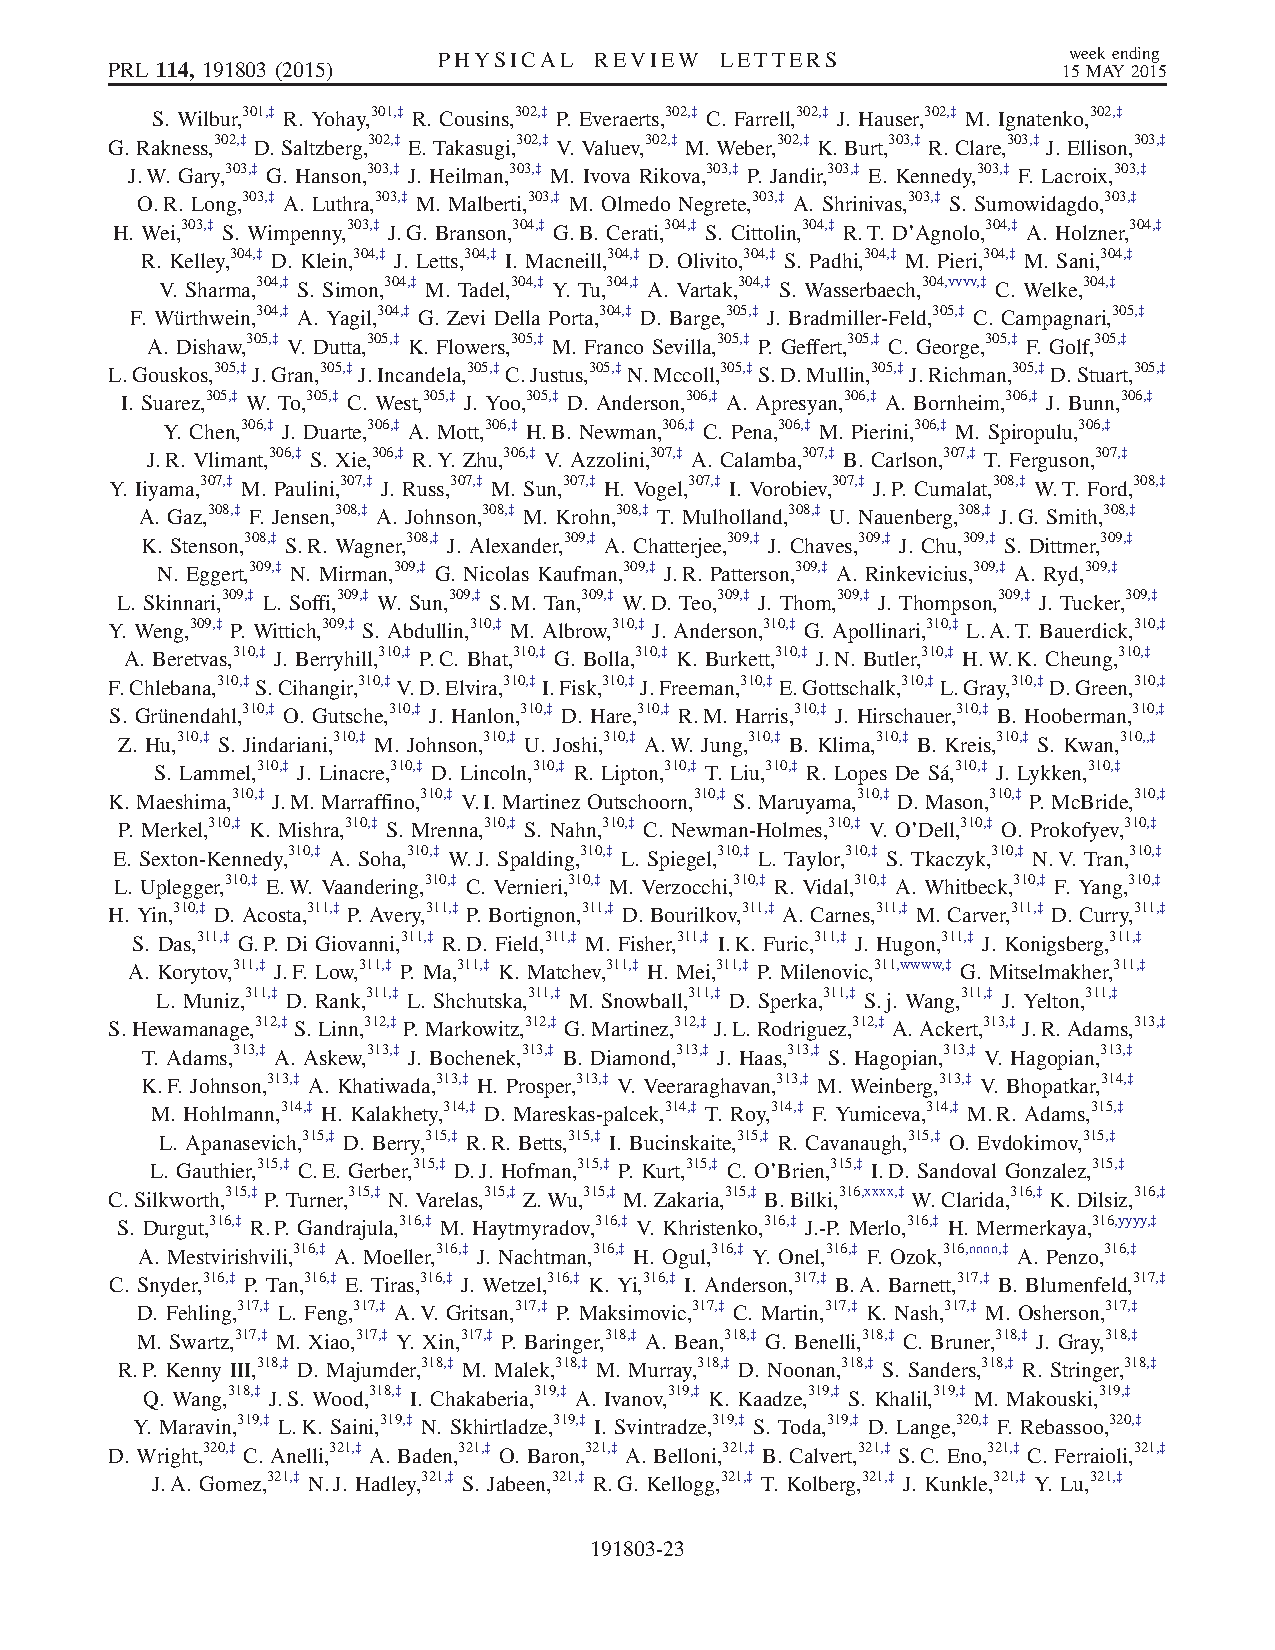
\includegraphics[height=\textheight]{figures/aad_combined_2015_authors_15}}
\only<16>{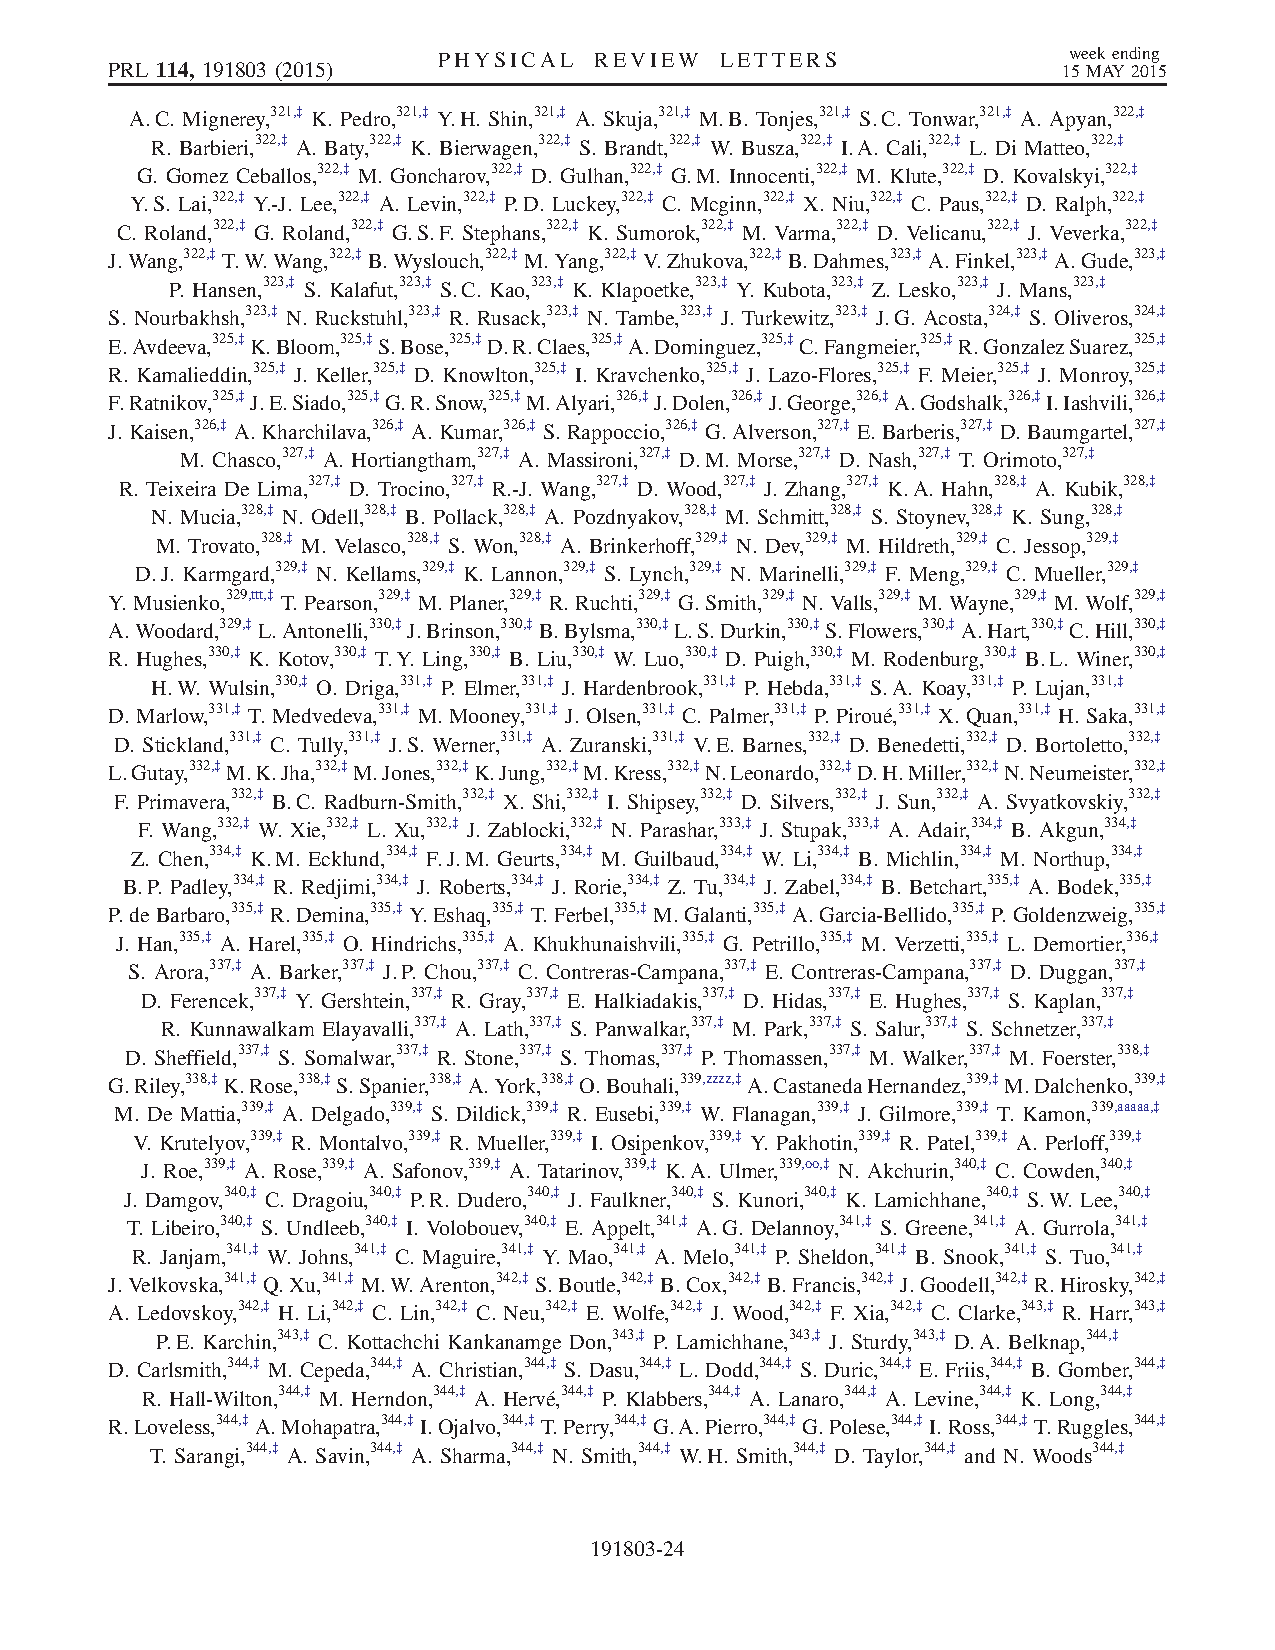
\includegraphics[height=\textheight]{figures/aad_combined_2015_authors_16}}
\end{center}

\end{frame}
%%%%%%%%%%%%%%%%%%%%%%%%%

\begin{frame}
Can we harness the power of mass collaboration in social science?
\end{frame}

\begin{frame}

\centering
\begin{tikzpicture}[x = \textwidth, y = \textheight]
\node at (0,0) {};
\node at (1,1) {};
% Life course visualization
\draw[->, line width = 2pt, gray] (.2,.85) -- (.8,.85);
\node[anchor = south] at (.5,.85) {Life course};
\node[anchor = north west, font = \footnotesize, align  = left] at (.2,.85) {Early\\experiences};
\node[anchor = north east, font = \footnotesize, align  = right] at (.8,.85) {Later\\outcomes};
% Standard approaches
\node<2->[anchor = north west, align = left] at (0,.7) {Standard social science practice};
\node<2->[anchor = west, font = \small] at (0,.6) {-- Describe social patterns};
\node<2->[anchor = west, font = \small] at (0,.55) {-- Theorize important factors};
\node<2->[anchor = west, font = \small] at (0,.5) {-- Estimate causal effects};
% Open questions
\node<3->[anchor = north west, align = left] at (.65,.7) {Open questions};
\node<4->[anchor = west, font = \small] at (.65,.6) {--};
\node<4->[anchor = west, font = \small, align = left] at (.68,.56) {Can we predict\\individual life\\outcomes?};
\node<5->[anchor = west, font = \small] at (.65,.45) {--};
\node<5->[anchor = west, font = \small, align = left] at (.68,.45) {Credibility};
% Illustration in data format
\node<6->[anchor = south, font = {\footnotesize\bf}] at (.35, .35) {Predictor variables};
\node<6->[anchor = south, font = {\footnotesize\bf}, rotate = 90] at (.1, .225) {Cases};
\draw<6->[rounded corners] (.1, .1) rectangle (.6,.35);
\node<6->[anchor = south, font = {\footnotesize\bf}] at (.8, .35) {Outcomes};
\draw<6->[rounded corners] (.7, .1) rectangle (.9,.35);
\draw<6->[->, line width = 4pt, gray] (.62, .225) -- (.68,.225);
% Illustrate picking a few predictors
\draw<7>[line width = 2pt, seagreen4] (.2,.1) -- (.2,.35);
\draw<7>[line width = 2pt, seagreen4] (.85,.1) -- (.85,.35);
\draw<8>[line width = 2pt, seagreen4] (.15,.1) -- (.15,.35);
\draw<8>[line width = 2pt, seagreen4] (.25,.1) -- (.25,.35);
\draw<8>[line width = 2pt, seagreen4] (.5,.1) -- (.5,.35);
\draw<8>[line width = 2pt, seagreen4] (.75,.1) -- (.75,.35);
\draw<9>[line width = 2pt, seagreen4] (.5,.1) -- (.5,.35);
\draw<9>[line width = 2pt, seagreen4] (.2,.1) -- (.2,.35);
\draw<9>[line width = 2pt, seagreen4] (.82,.1) -- (.82,.35);
\end{tikzpicture}

\end{frame}

\begin{frame}

\begin{center}

\includegraphics[width=\textwidth]{figures/ff_logo}
\end{center}

\begin{itemize}
\item Birth cohort panel study
\item $\approx$ 5,000 children born in 20 U.S. cities
\item Followed from birth through age 15
\end{itemize}

\end{frame}
%%%%%%%%%%%%%%%%%%%%%%%%%

\begin{frame}

\begin{center}
\includegraphics<1>[height=0.8\textheight]{figures/ff_design_public_b9}
\includegraphics<2>[height=0.8\textheight]{figures/ff_design_public2}
\end{center}

\end{frame}
%%%%%%%%%%%%%%%%%%%%%%%%%
\begin{frame}

Six age 15 outcomes:
\begin{itemize}
\item GPA
\item Material Hardship
\item Grit
\item Evicted
\item Job training
\item Job loss
\end{itemize}

\end{frame}
%%%%%%%%%%%%%%%%%%%%%%%%%
\begin{frame}

\begin{center}
%\includegraphics<1>[width=\textwidth]{figures/ff_design_matrix_ml}
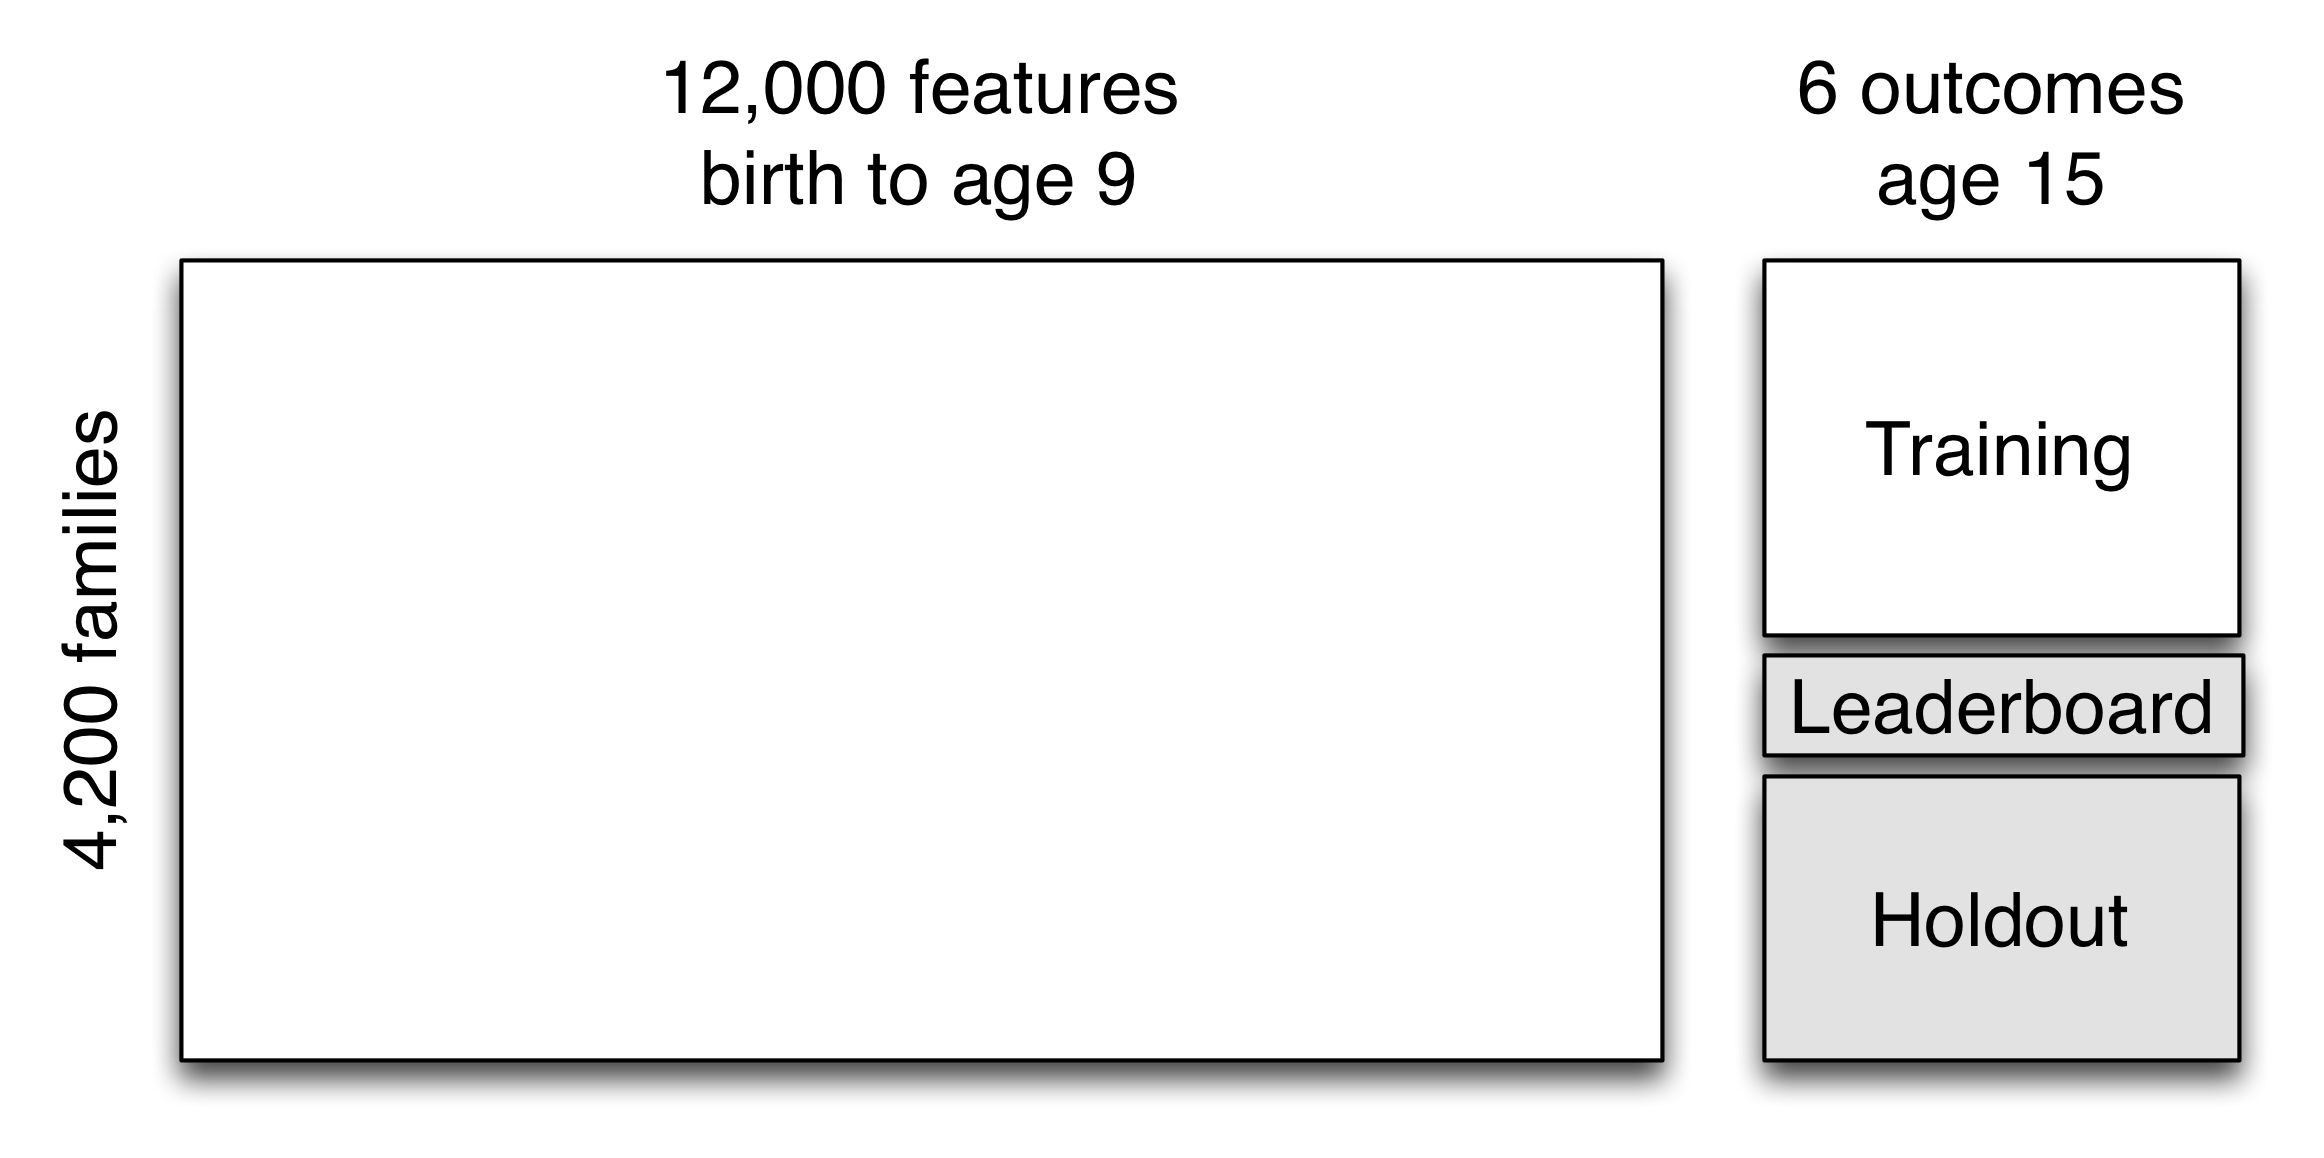
\includegraphics[width=\textwidth]{figures/ffc_design_matrix_ml}
\end{center}

\end{frame}
%%%%%%%%%%%%%%%%%%%%%%%%%
\begin{frame}

441 registered participants
\begin{itemize}
\item social scientists and data scientists
\item undergraduates, grad students, and professionals
\item many working in teams
\end{itemize}

\end{frame}
%%%%%%%%%%%%%%%%%%%%%%%%%%%
\begin{frame}

\begin{center}
How did they do?
\end{center}

\end{frame}
%%%%%%%%%%%%%%%%%%%%%%%%%%%
\begin{frame}
\centering
\begin{tikzpicture}[x = \textwidth, y = \textheight]
\node<1>[anchor = north] at (.5,1) {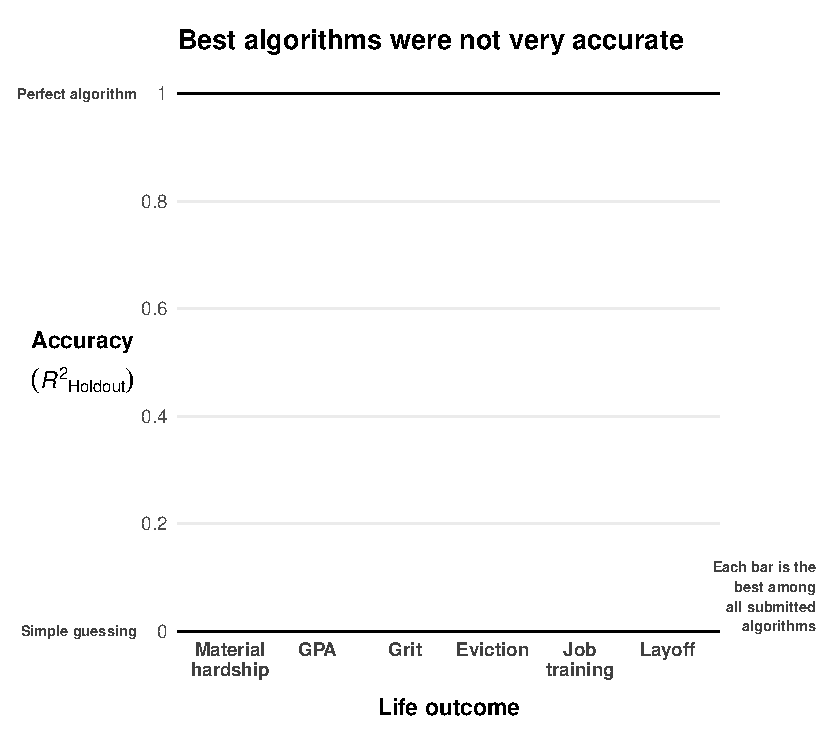
\includegraphics[width=\textwidth]{figures/image0}};
\draw<1>[fill = white, color = white] (.2,.9) rectangle (.85,.95);
\node<1> at (.55,.5) {$R^2_\text{Holdout} = 1 - \frac{\sum_{i\in\text{Holdout}} \left(y_i - \hat{y}_i\right)^2}{\sum_{i\in\text{Holdout}} \left(y_i - \bar{y}_\text{Training}\right)^2}$};
\node<2-6>[anchor = north] at (.5,1) {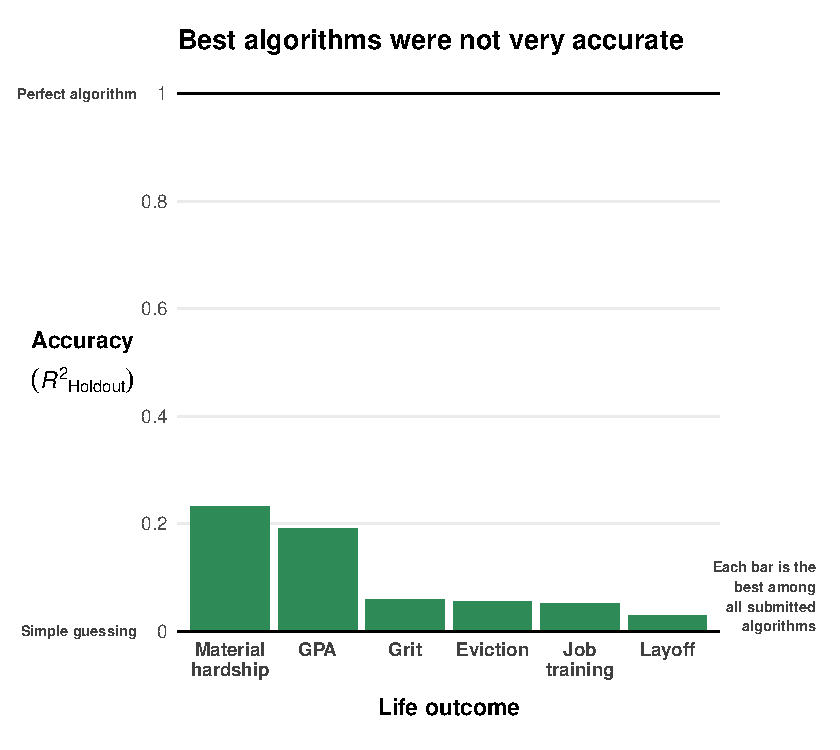
\includegraphics[width=\textwidth]{figures/image1}};
\node<3>[draw, rounded corners, fill = white] at (.63,.55) {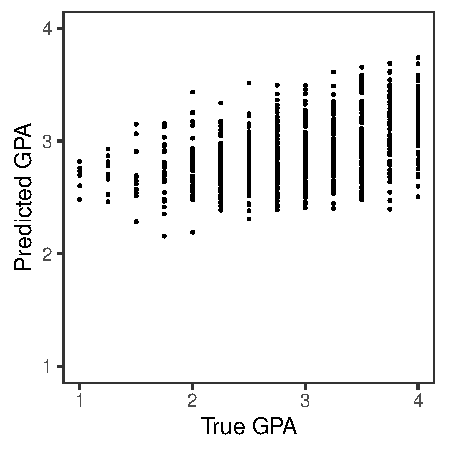
\includegraphics[height = .5\textheight]{figures/gpa_best_scatter}};
\node<4>[draw, rounded corners, fill = white] at (.63,.55) {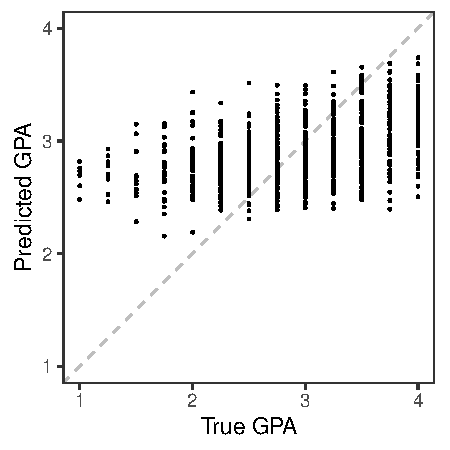
\includegraphics[height = .5\textheight]{figures/gpa_best_scatter_diagonal}};
\node<5>[draw, rounded corners, fill = white] at (.63,.55) {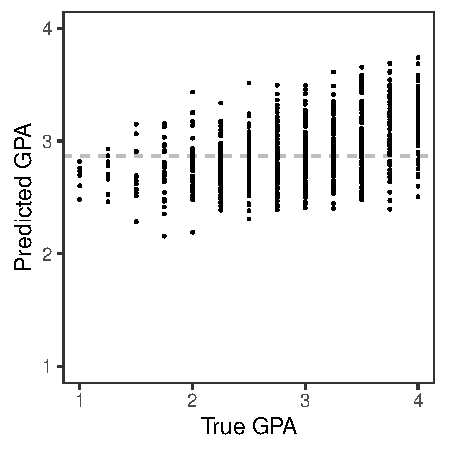
\includegraphics[height = .5\textheight]{figures/gpa_best_scatter_horizontal}};
\node<7>[anchor = north] at (.5,1) {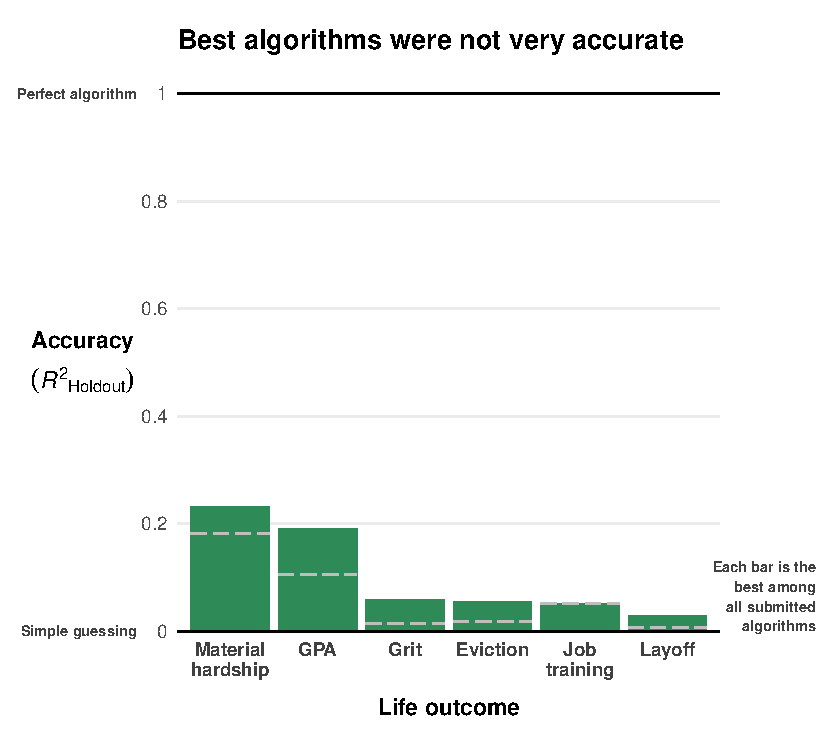
\includegraphics[width=\textwidth]{figures/image1a}};
\end{tikzpicture}
\end{frame}

%%%%%%%%%%%%%%%%%%%%%%%%%%%
\begin{frame}
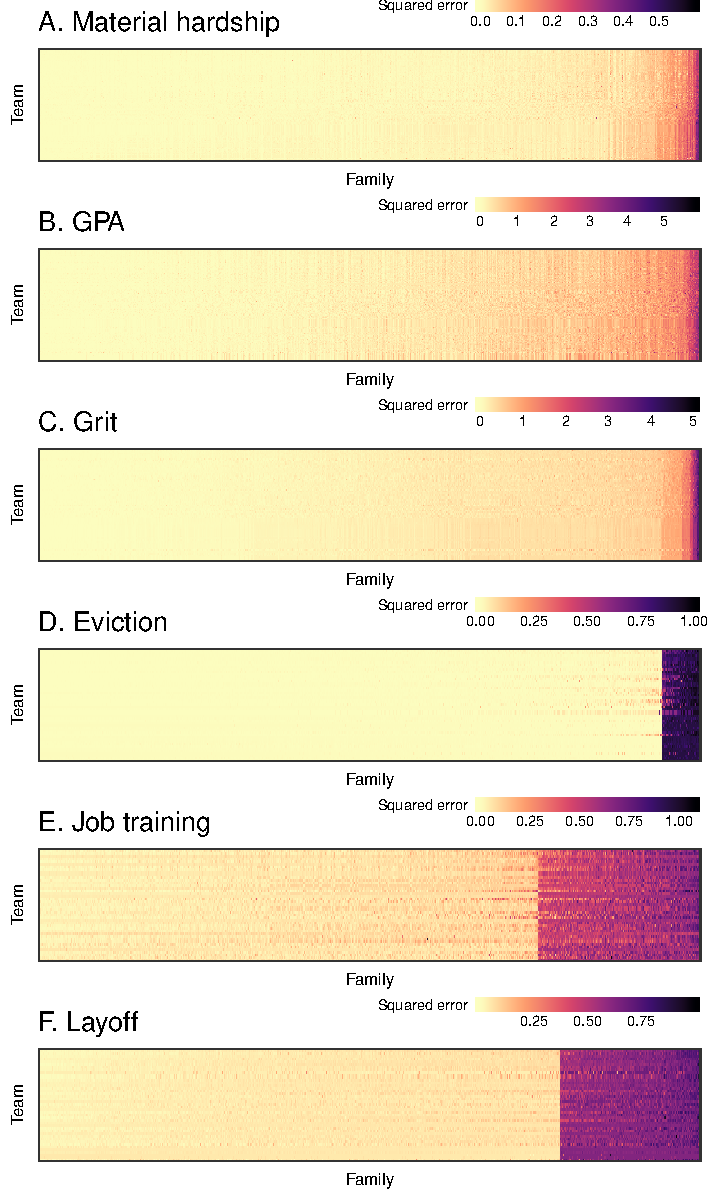
\includegraphics[width = \textwidth, trim = {0 5.37in 0 1.3in}, clip]{figures/4_heatmaps_sqerr_6outcomes}
\end{frame}

%%%%%%%%%%%%%%%%%%%%%%%%%%%
\begin{frame}
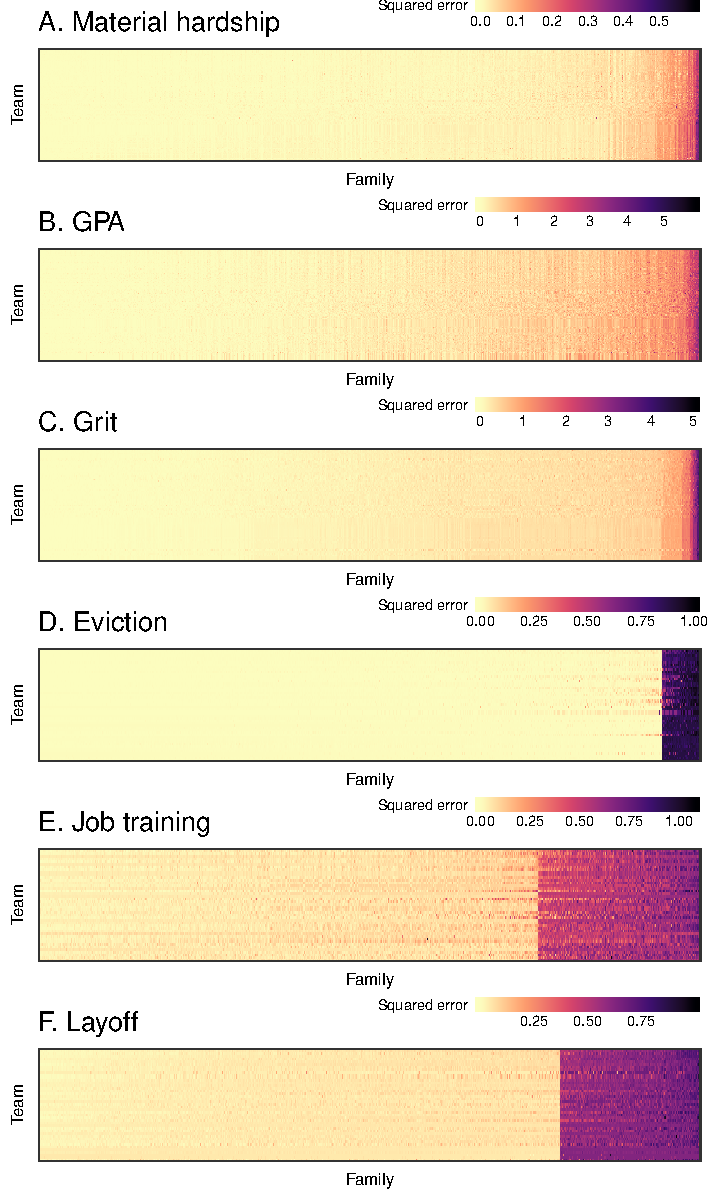
\includegraphics[width = \textwidth, trim = {0 2.72in 0 3.95in}, clip]{figures/4_heatmaps_sqerr_6outcomes}
\end{frame}

%%%%%%%%%%%%%%%%%%%%%%%%%%%
\begin{frame}
% Blank slide for separation
\end{frame}

%%%%%%%%%%%%%%%%%%%%%%%%%%%
\begin{frame}
What do these results mean for policy and for science?
\end{frame}

%%%%%%%%%%%%%%%%%%%%%%%%%%%
\begin{frame}
\begin{tikzpicture}[x = \textwidth, y = \textheight]
\node at (0,0) {};
\node at (1,1) {};
\node[anchor = north west, align = left] at (0,.83) {For \bblue{policymakers},};
\node<2->[anchor = north west, align = left] at (0,.68) {-- Do not assume that predictive algorithms are accurate};
\node<3->[anchor = north west, align = left] at (0,.58) {-- Transparent evaluation of any algorithm is needed};
\node<4->[anchor = north west, align = left] at (0,.48) {-- Complex models may not outperform simple models};
\end{tikzpicture}
\end{frame}

%%%%%%%%%%%%%%%%%%%%%%%%%%%
\begin{frame}
\begin{tikzpicture}[x = \textwidth, y = \textheight]
\node at (0,0) {};
\node at (1,1) {};
\node[anchor = north west] at (0,.95) {For \bblue{scientists}: A paradox of prediction and understanding};
\node<2->[anchor = north west, align = left] at (0,.83) {These data have\\generated\\understanding...};
\node<2->[anchor = north, font = \footnotesize] at (0.15,.63) {(hundreds of papers)};
\draw<2->[->, thick] (.15,.63) -- (.13,.66);
\node<3->[anchor = north east, align = right] at (1,.83) {...yet the very same data\\did not yield accurate\\predictions};
\node<3->[anchor = north, font = \footnotesize] at (0.85,.63) {(our result)};
\draw<3->[->, thick] (.85,.63) -- (.87,.66);
\node<4->[anchor = north west, align = left] at (0,.52) {\bblue{Resolutions:}};
\node<5->[anchor = north east, font = \small] at (0.04,.45) {1. };
\node<5->[anchor = north west, align = left, font = \small] at (.04,.45) {If understanding implies an ability to predict,\\then \bgreen{we do not understand} the life course.};
\node<6->[anchor = north east, font = \small] at (0.04,.34) {2. };
\node<6->[anchor = north west, align = left, font = \small] at (.04,.34) {Perhaps we have \bgreen{understanding despite poor prediction}.};
\node<6->[anchor = north west, align = left, font =  \footnotesize] at (.06,.29) {-- Aggregate description\\-- Causal effects};
\node<7->[anchor = north east, font = \small] at (0.04,.18) {3. };
\node<7->[anchor = north west, align = left, font = \small] at (.04,.18) {Our understanding is correct but \bgreen{incomplete}.\\We need theories that point toward poor prediction};
\end{tikzpicture}
\end{frame}

%%%%%%%%%%%%%%%%%%%%%%%%%%%
\begin{frame}
\begin{tikzpicture}[x = \textwidth, y = \textheight]
\node at (0,0) {};
\node at (1,1) {};
\node[anchor = north west] at (0,.95) {For \bblue{scientists}: The value of mass collaboration};
\node<2->[anchor = south west, align = left] at (0, .65) {A credible estimate of predictability};
\node<3->[anchor = west, align = left] at (0, .5) {The common task framework does not end\\with choosing the winner};
\node<4->[anchor = north west, align = left] at (0, .35) {There may be other problems we can solve\\better collectively than individually};
\end{tikzpicture}
\end{frame}

%%%%%%%%%%%%%%%%%%%%%%%%%%%
\begin{frame}
\centering
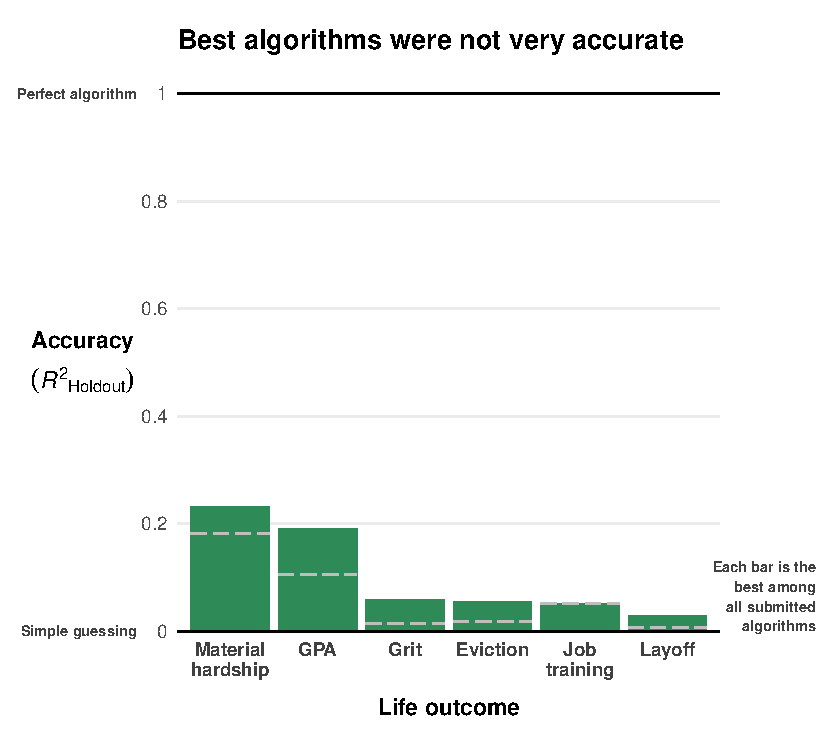
\includegraphics[width=\textwidth]{figures/image1a}

\end{frame}


\begin{frame}
\huge

Generalizing: Estimator selection by sample splitting

\end{frame}

\begin{frame}{Task}

\begin{itemize}
\item 10 sampled players per MLB team
\item estimate the mean salary among the Dodgers
\end{itemize}

\end{frame}

\begin{frame}{Estimator: k-nearest neighbors}

10 sampled players per team
\begin{itemize}
\item Dodger sample mean might be noisy
\item Could pool with similar teams defined by past mean salary
\begin{itemize}
\item Dodgers: 8.39m
\item 1st-nearest neighbor. NY Mets: 8.34m
\item 2nd-nearest neighbor. NY Yankees: 7.60m
\item 3rd-nearest neighbor. Philadelphia: 6.50m
\end{itemize}
\item How does performance change with the number of neighbors included?
\begin{itemize}
\item measured by mean squared prediction error
\end{itemize}
\end{itemize}

\end{frame}

\begin{frame}
\includegraphics<1>[width = \textwidth]{figures/knn_0}
\includegraphics<2>[width = \textwidth]{figures/knn_1}
\includegraphics<3>[width = \textwidth]{figures/knn_2}
\includegraphics<4>[width = \textwidth]{figures/knn_3}
\includegraphics<5>[width = \textwidth]{figures/knn_4}
\includegraphics<6>[width = \textwidth]{figures/knn_5}
\includegraphics<7>[width = \textwidth]{figures/knn_10}
\includegraphics<8>[width = \textwidth]{figures/knn_15}
\includegraphics<9>[width = \textwidth]{figures/knn_20}
\includegraphics<10>[width = \textwidth]{figures/knn_25}
\end{frame}

\begin{frame}
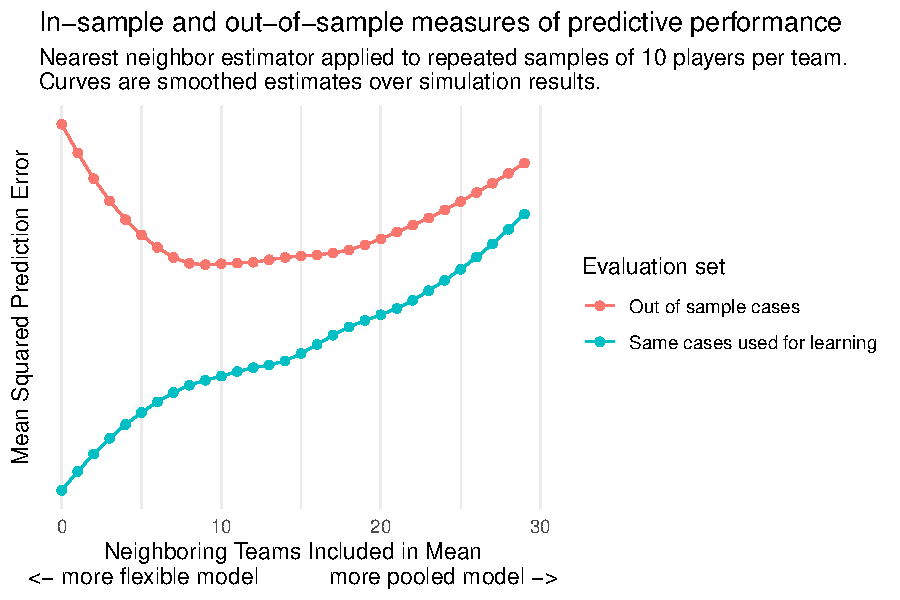
\includegraphics[width = \textwidth]{figures/knn_29}
\end{frame}

\section{Sample Splitting}

\begin{frame}
You have one sample.\\
How do you estimate out-of-sample performance?
\end{frame}

\begin{frame}
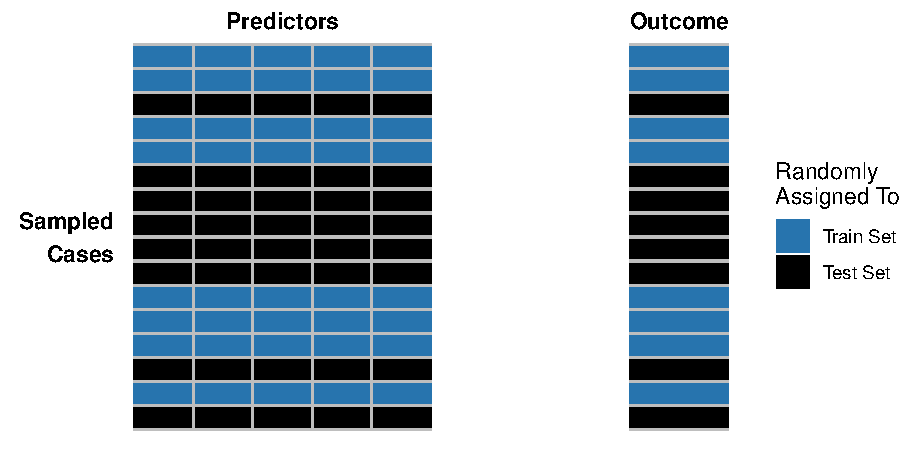
\includegraphics[width = \textwidth]{figures/randomize_split}
\end{frame}

\begin{frame}
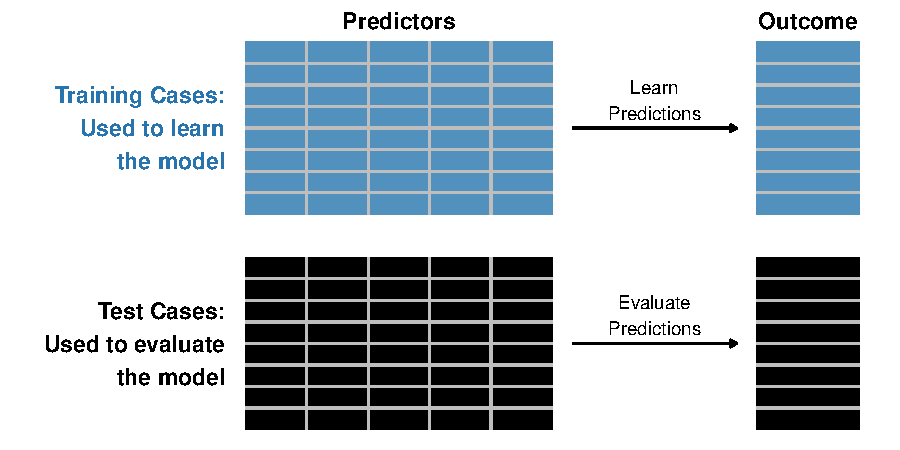
\includegraphics[width = \textwidth]{figures/train_test}
\end{frame}

\begin{frame}{Exercise: Conduct a sample split in code}

\begin{enumerate}
\item Sample 10 players per team
\item Take a 50-50 sample split stratified by team
\item Fit a linear regression in the train set
\item Predict in the test set
\item Report mean squared error
\end{enumerate}

\end{frame}

\section{Cross Validation}


\begin{frame}{Cross Validation}

A train test split loses lots of data to testing. \vskip .2in
Is there a way to bring it back?

\end{frame}

\begin{frame}{Cross Validation}
\begin{tikzpicture}[x = \textwidth, y = .8\textheight]
\node at (0,0) {};
\node at (1,1) {};
\node[anchor = north west, align = center] at (0,1) {Randomize\\to 5 folds};
\node[anchor = north west] at (0,.9) {
\includegraphics[scale = .8]{figures/five_folds}};
\node<2->[anchor = north, align = center] at (.55,1) {Iteratively use each as the test set};
\node<3->[anchor = north west] at (.2,.9) {
\includegraphics[scale = .8]{figures/five_folds_1}};
\node<4->[anchor = north west] at (.35,.9) {
\includegraphics[scale = .8]{figures/five_folds_2}};
\node<5->[anchor = north west] at (.5,.9) {
\includegraphics[scale = .8]{figures/five_folds_3}};
\node<6->[anchor = north west] at (.65,.9) {
\includegraphics[scale = .8]{figures/five_folds_4}};
\node<7->[anchor = north west] at (.8,.9) {
\includegraphics[scale = .8]{figures/five_folds_5}};
\node<8->[anchor = north, align = center] at (.55,.1) {Average prediction error over folds};
\end{tikzpicture}
\end{frame}

\begin{frame}
Out-of-sample predictive performance is not just for tuning parameters. \vskip .2in
It can help you choose your algorithm.
\end{frame}

\begin{frame}
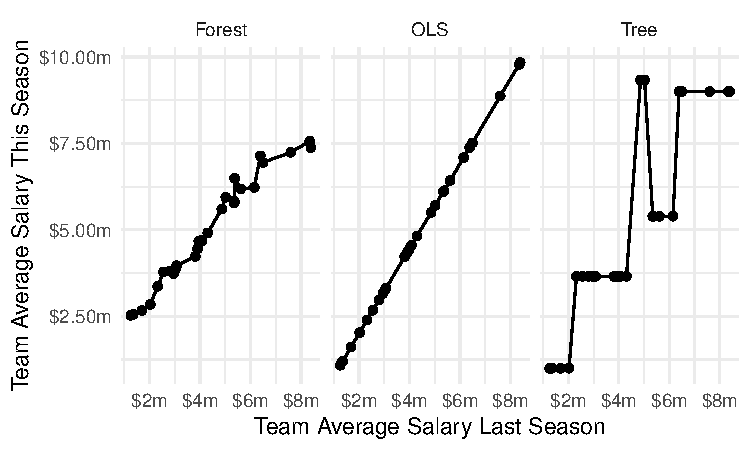
\includegraphics[width = \textwidth]{figures/many_algorithm_predictions}
\end{frame}

\begin{frame}
\includegraphics[width = \textwidth]{figures/many_algorithm_mse}
\end{frame}

\goalsframe

%%%%%%%%%
%  APPENDIX	%
%%%%%%%%%

\begin{frame}
\centering \huge Appendix
\end{frame}

\begin{frame}{Appendix}
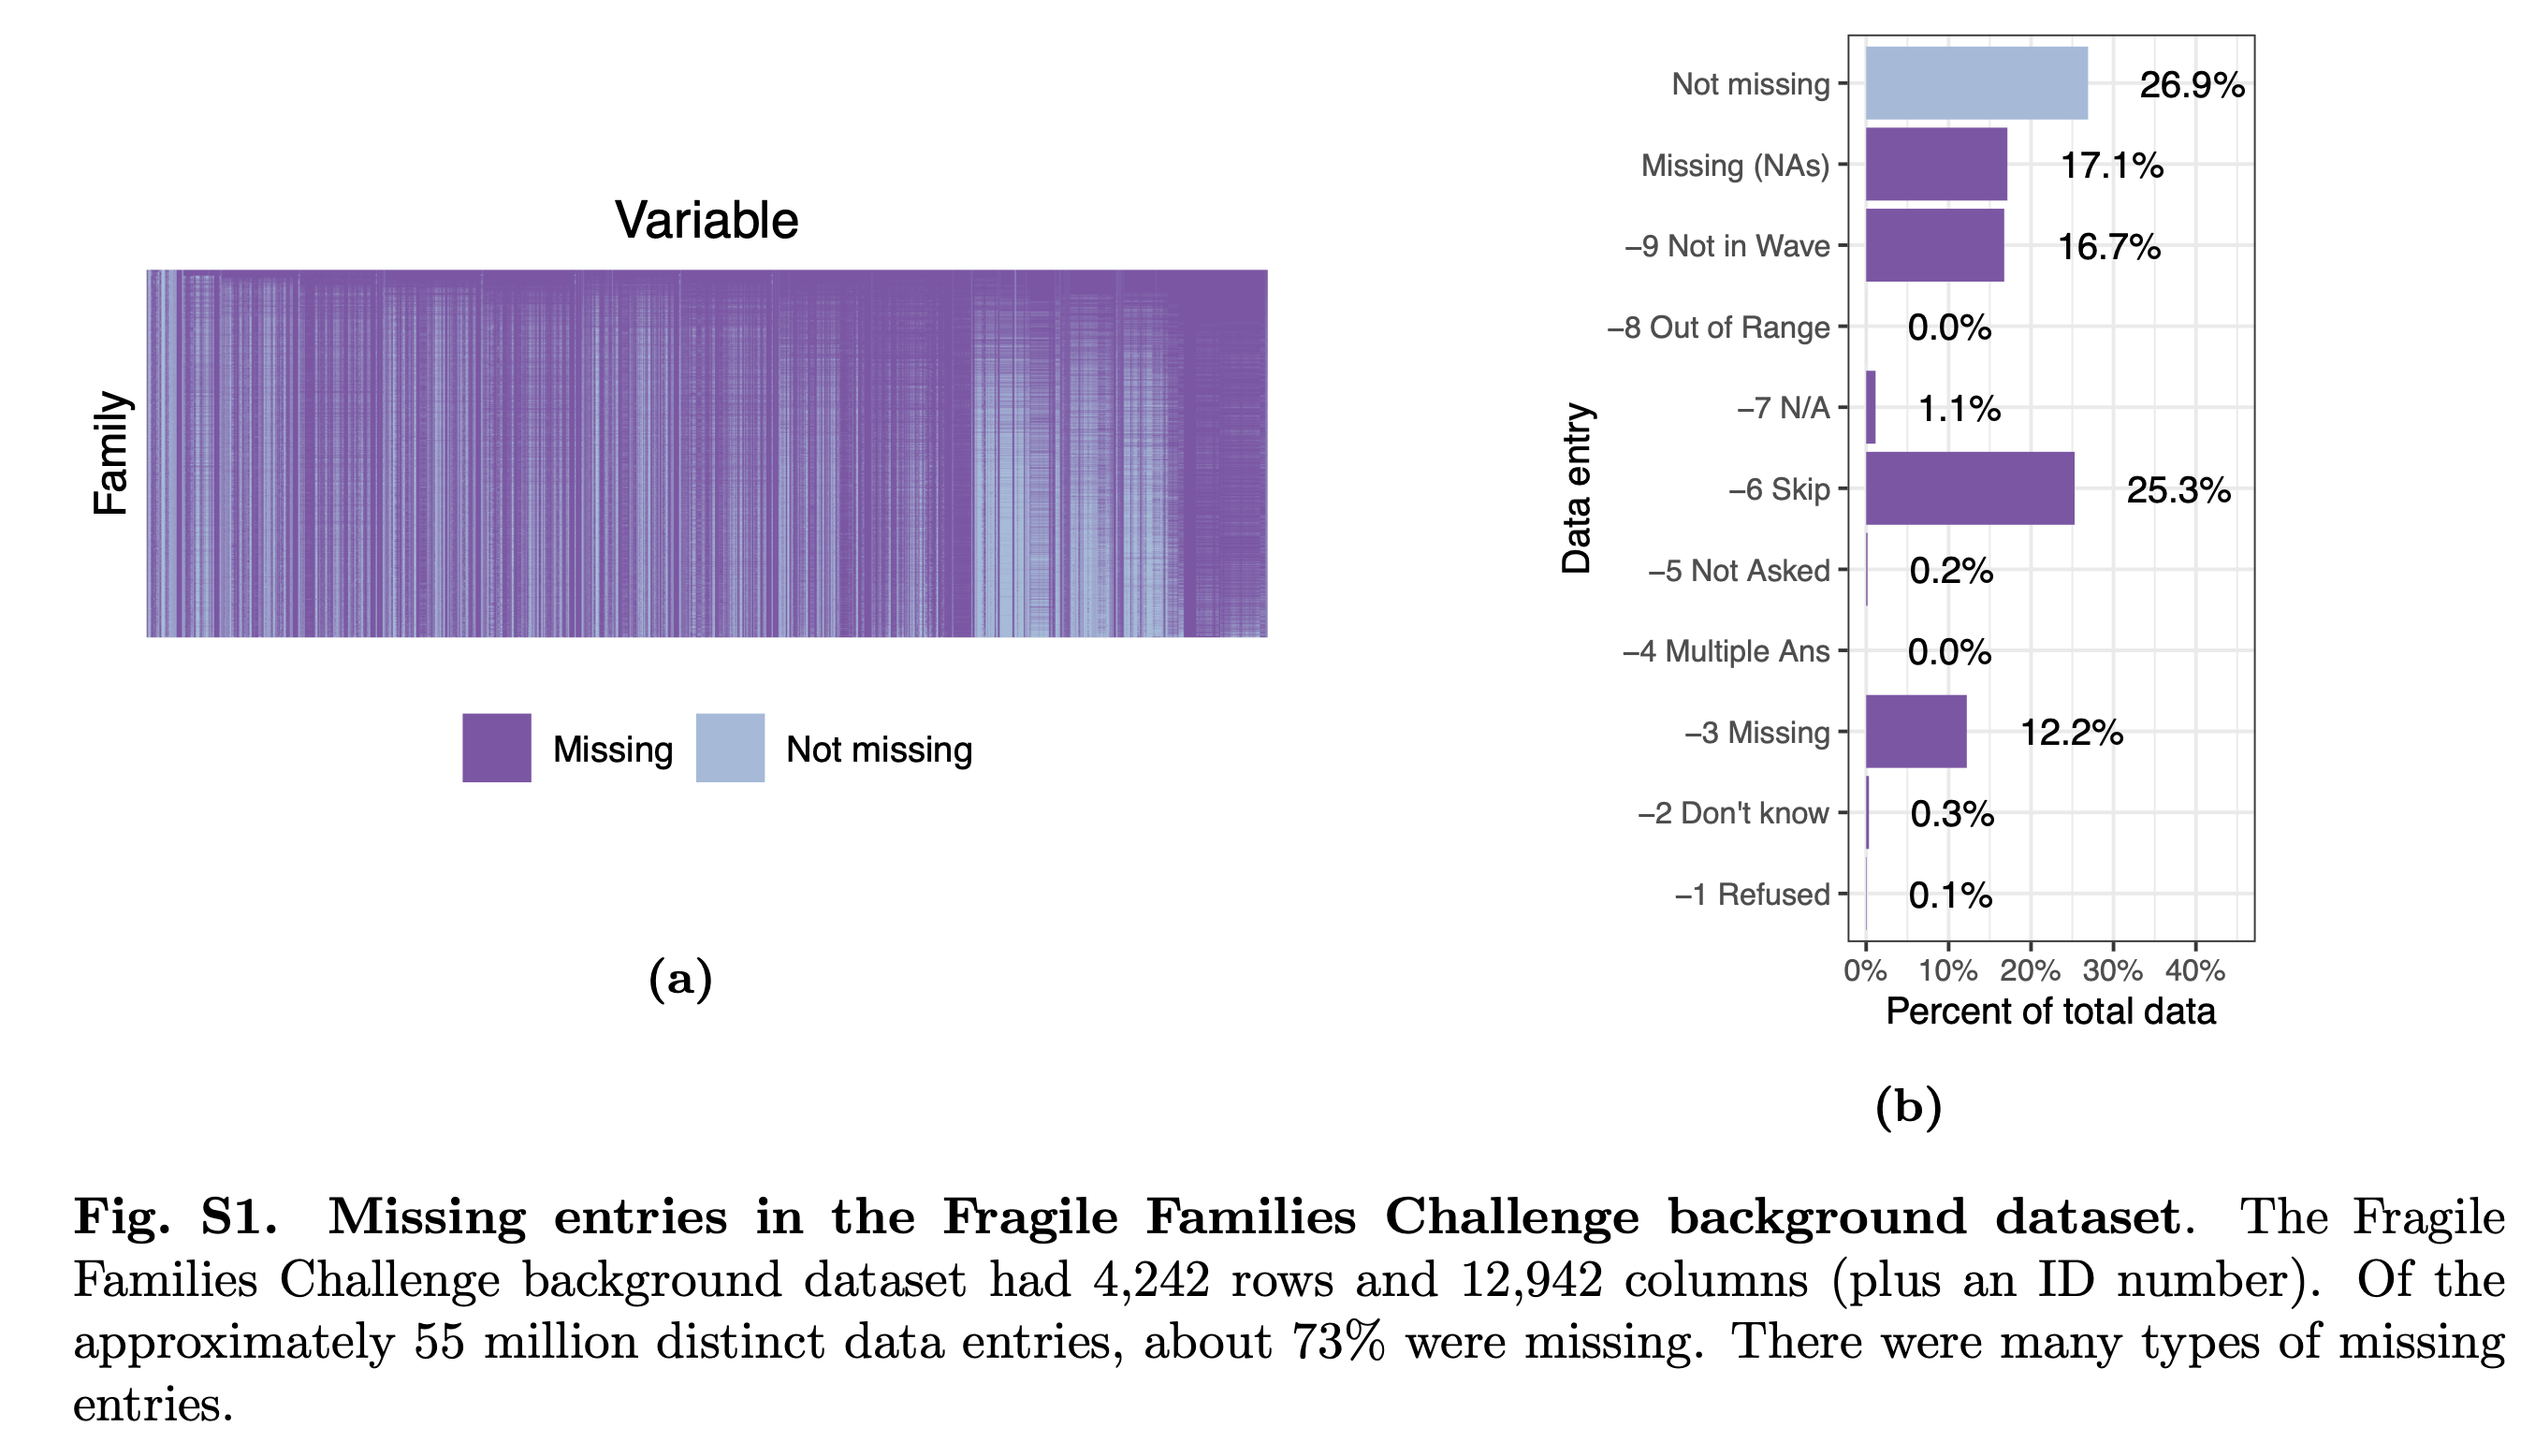
\includegraphics[width = \textwidth]{figures/si_missing_data}
\end{frame}

\begin{frame}{Appendix}
\centering
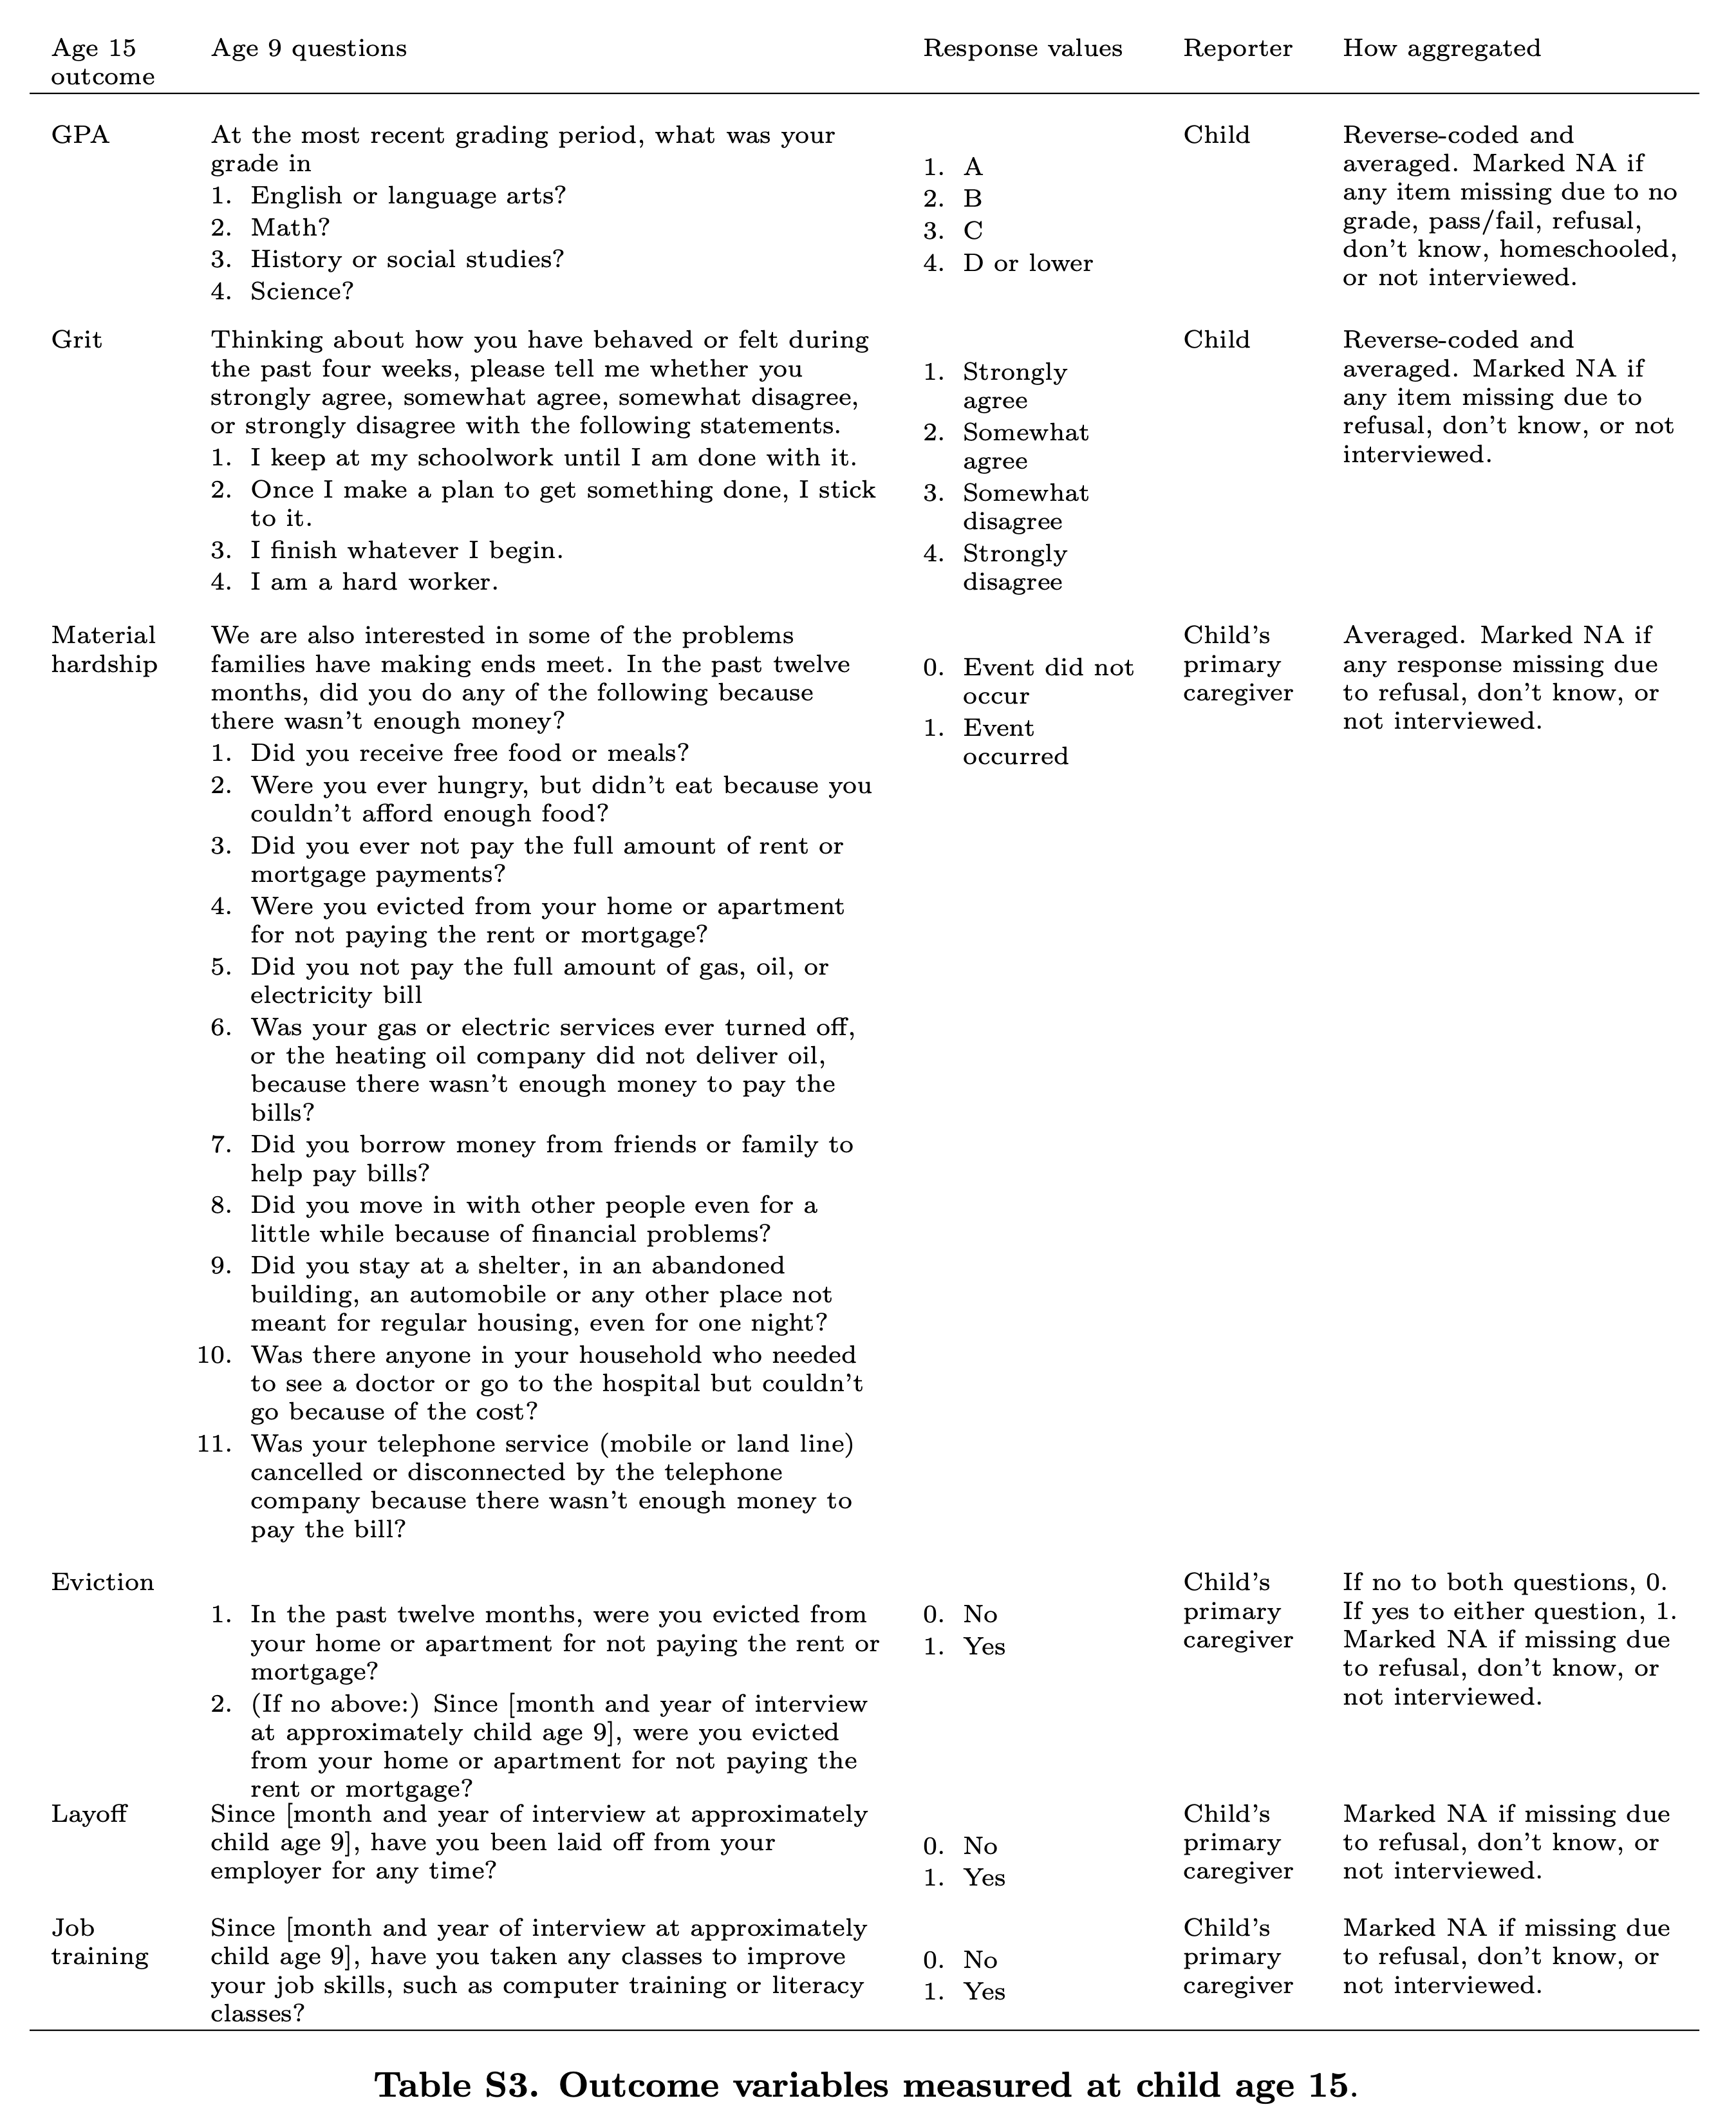
\includegraphics[height = .8\textheight]{figures/si_outcome_text}
\end{frame}

\begin{frame}{Appendix}
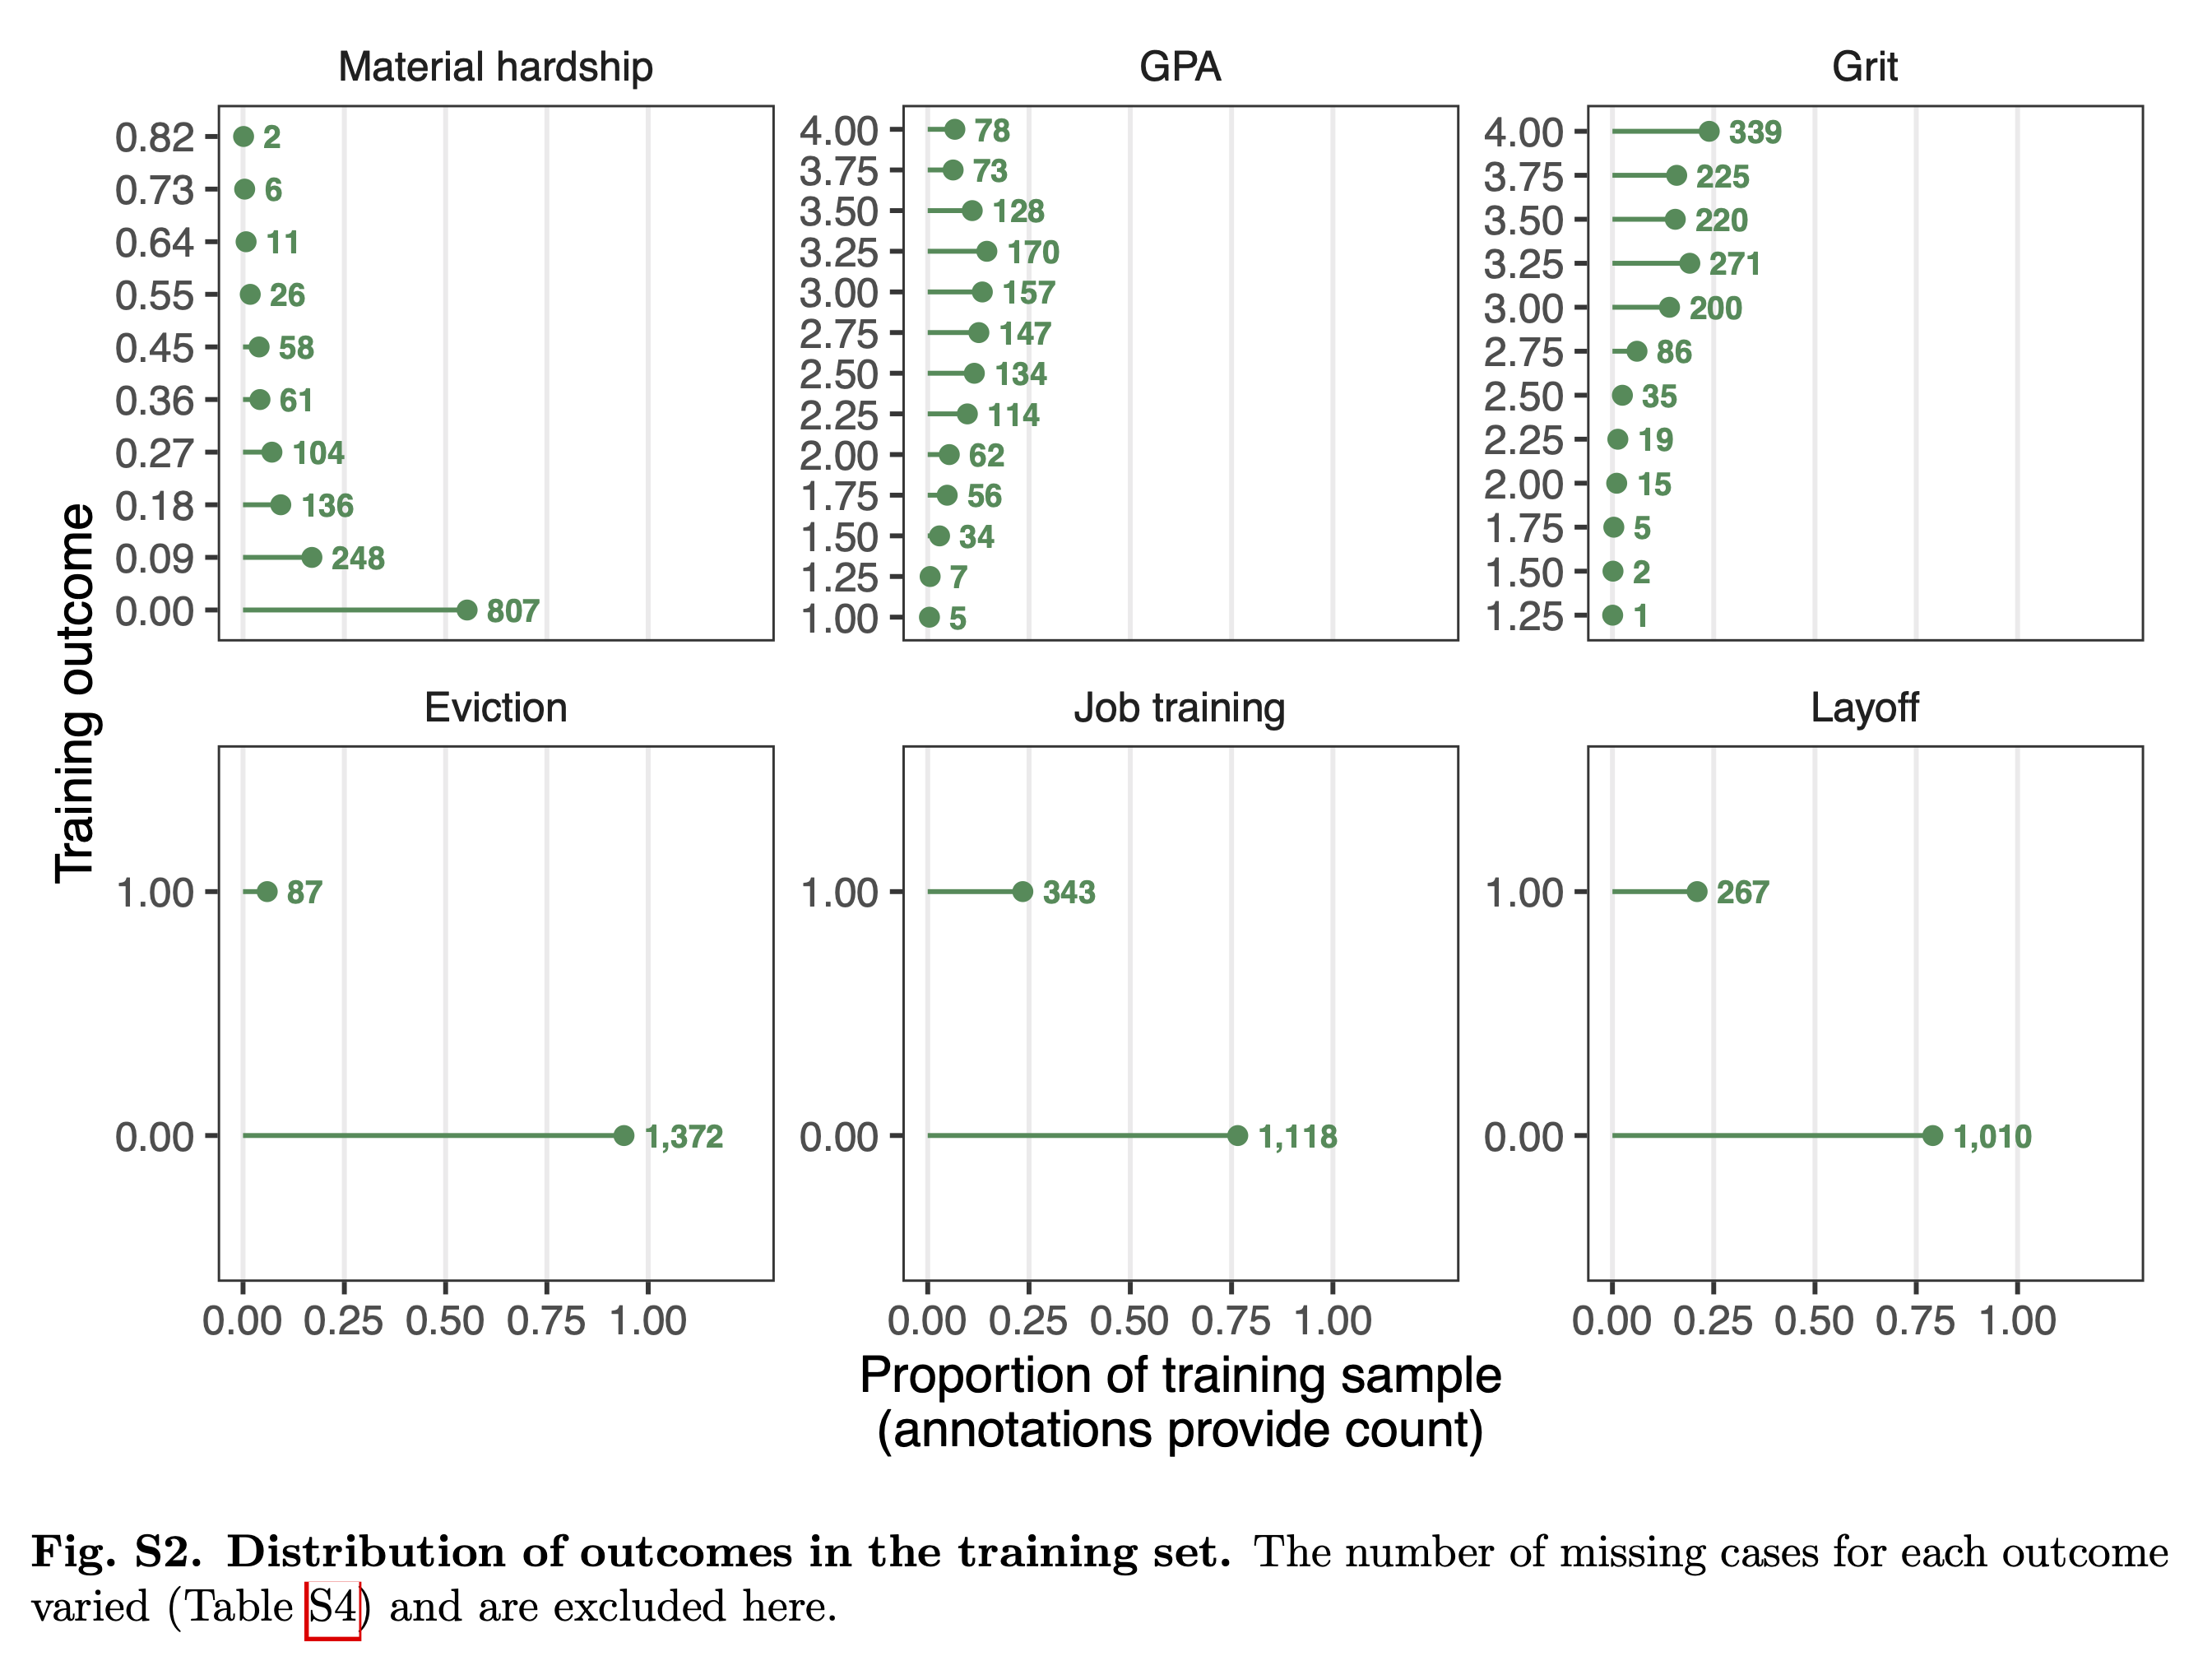
\includegraphics[width = \textwidth]{figures/si_outcome_histograms}
\end{frame}

\begin{frame}{Appendix}
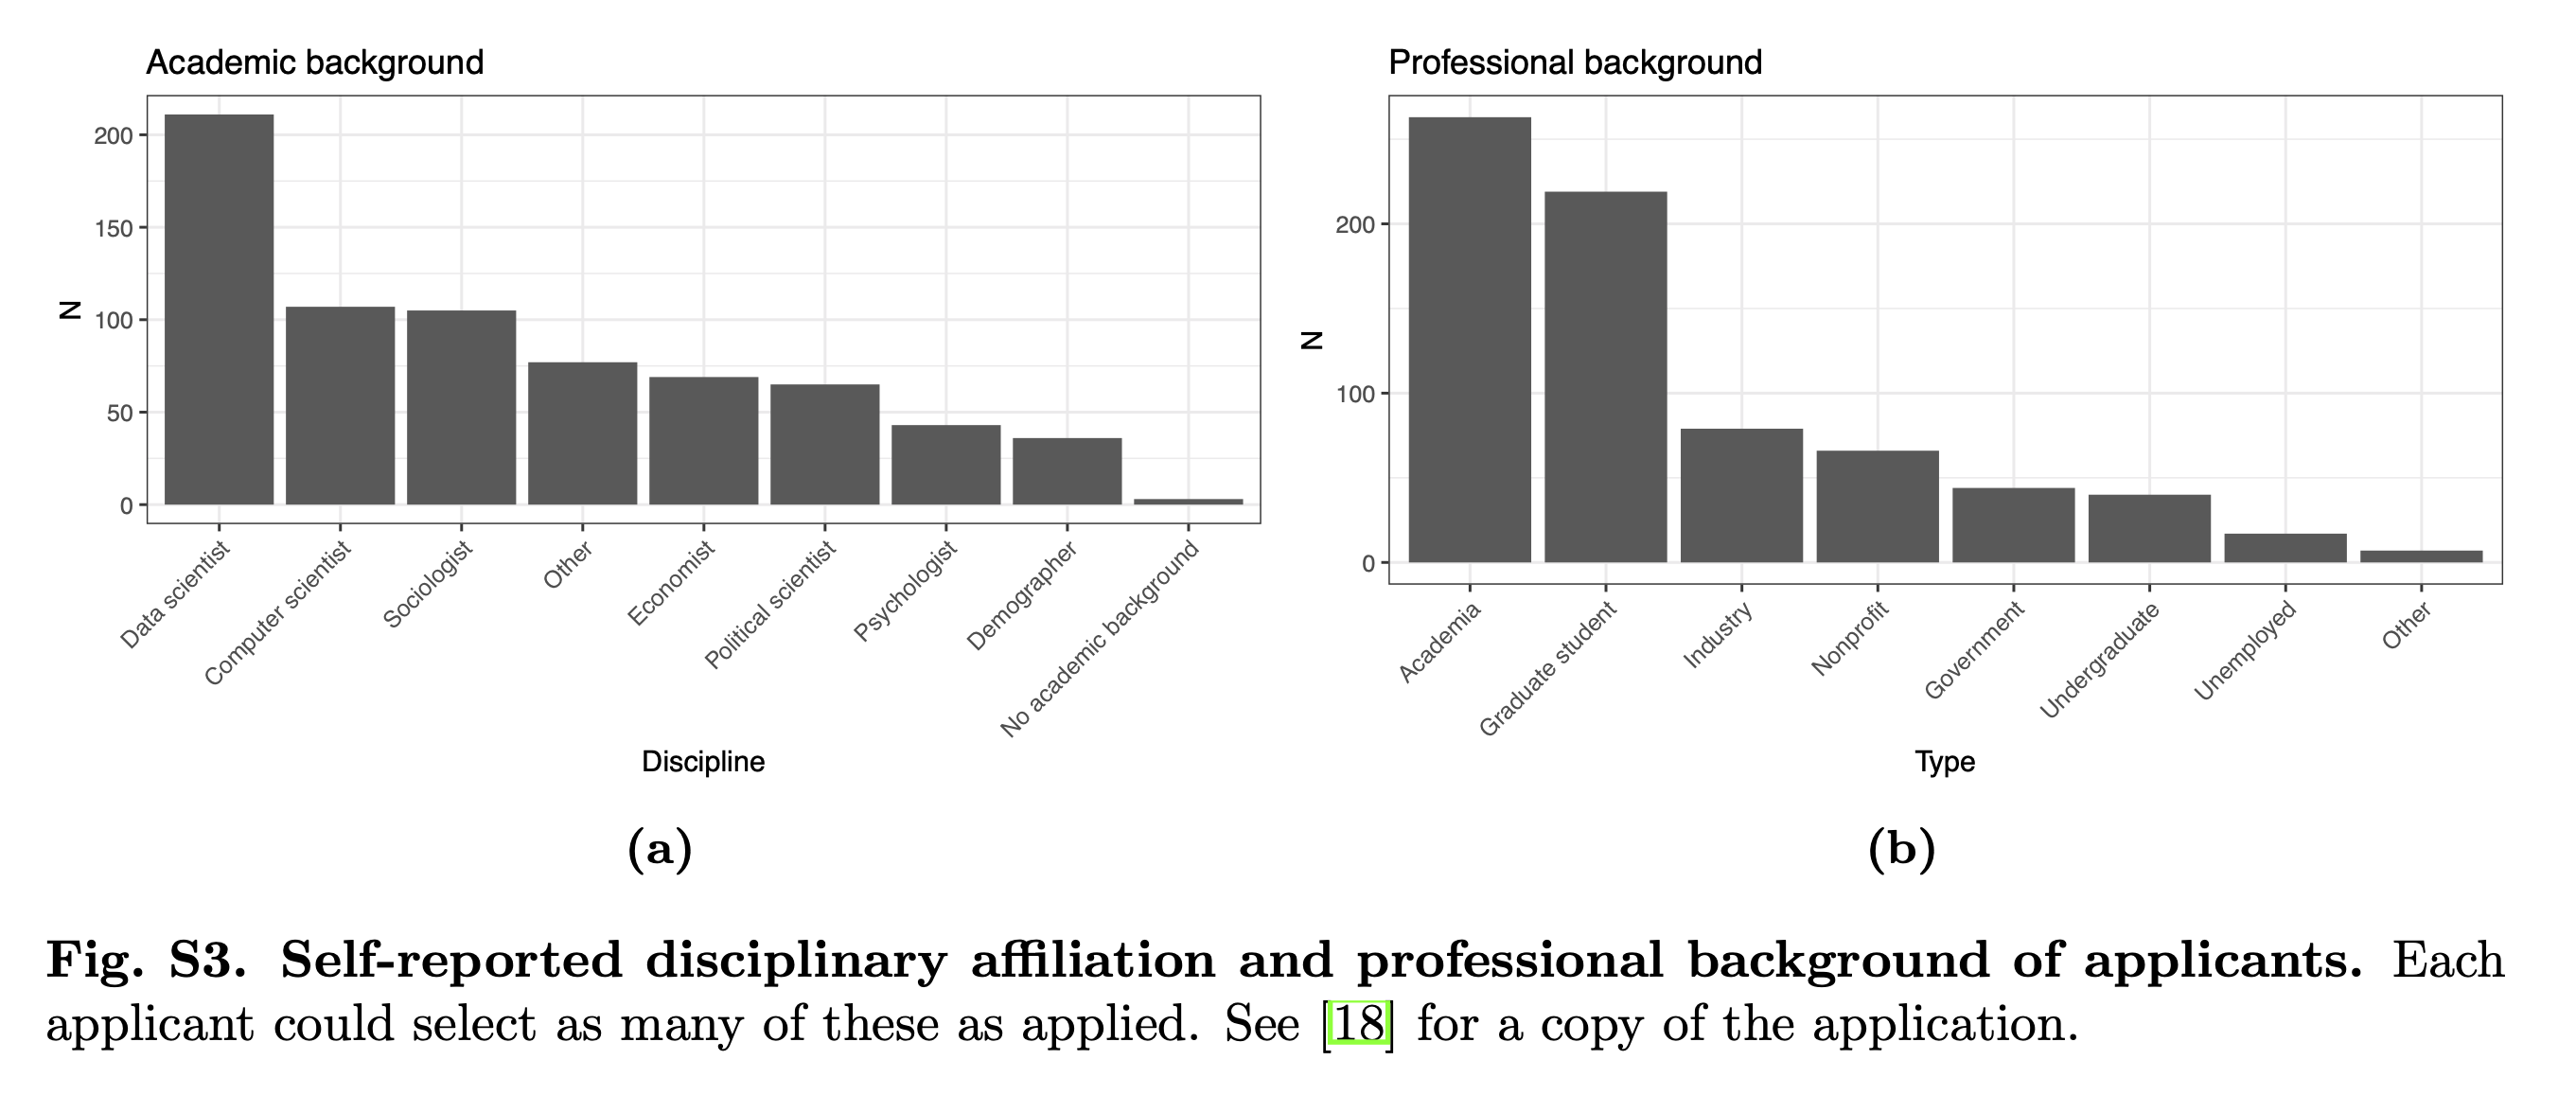
\includegraphics[width = \textwidth]{figures/si_disciplines}
\end{frame}

\begin{frame}{Appendix}
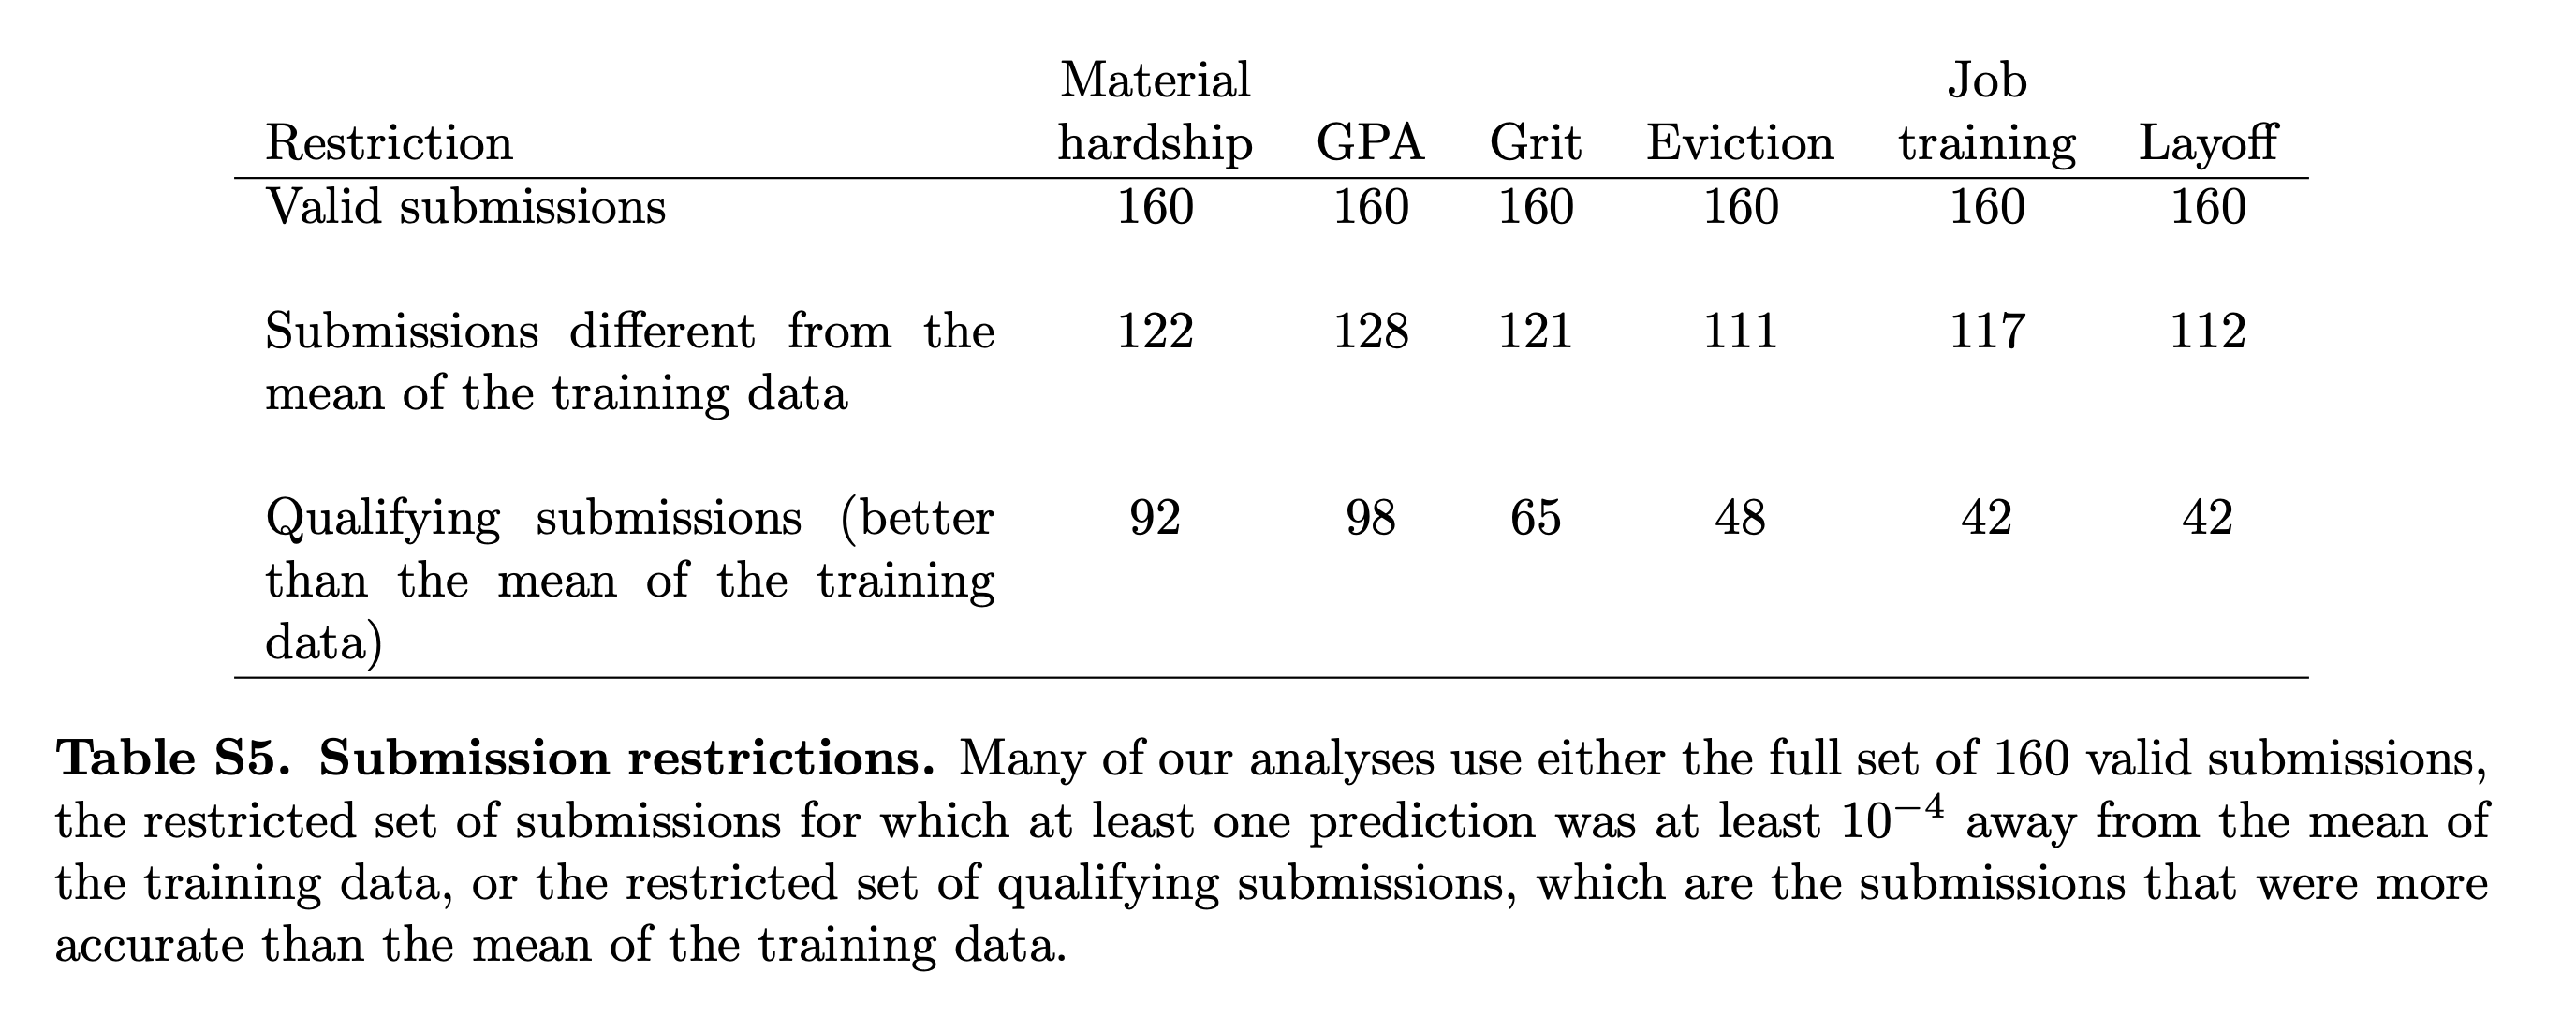
\includegraphics[width = \textwidth]{figures/si_qualifying_table}
\end{frame}

\begin{frame}{Appendix}
\centering
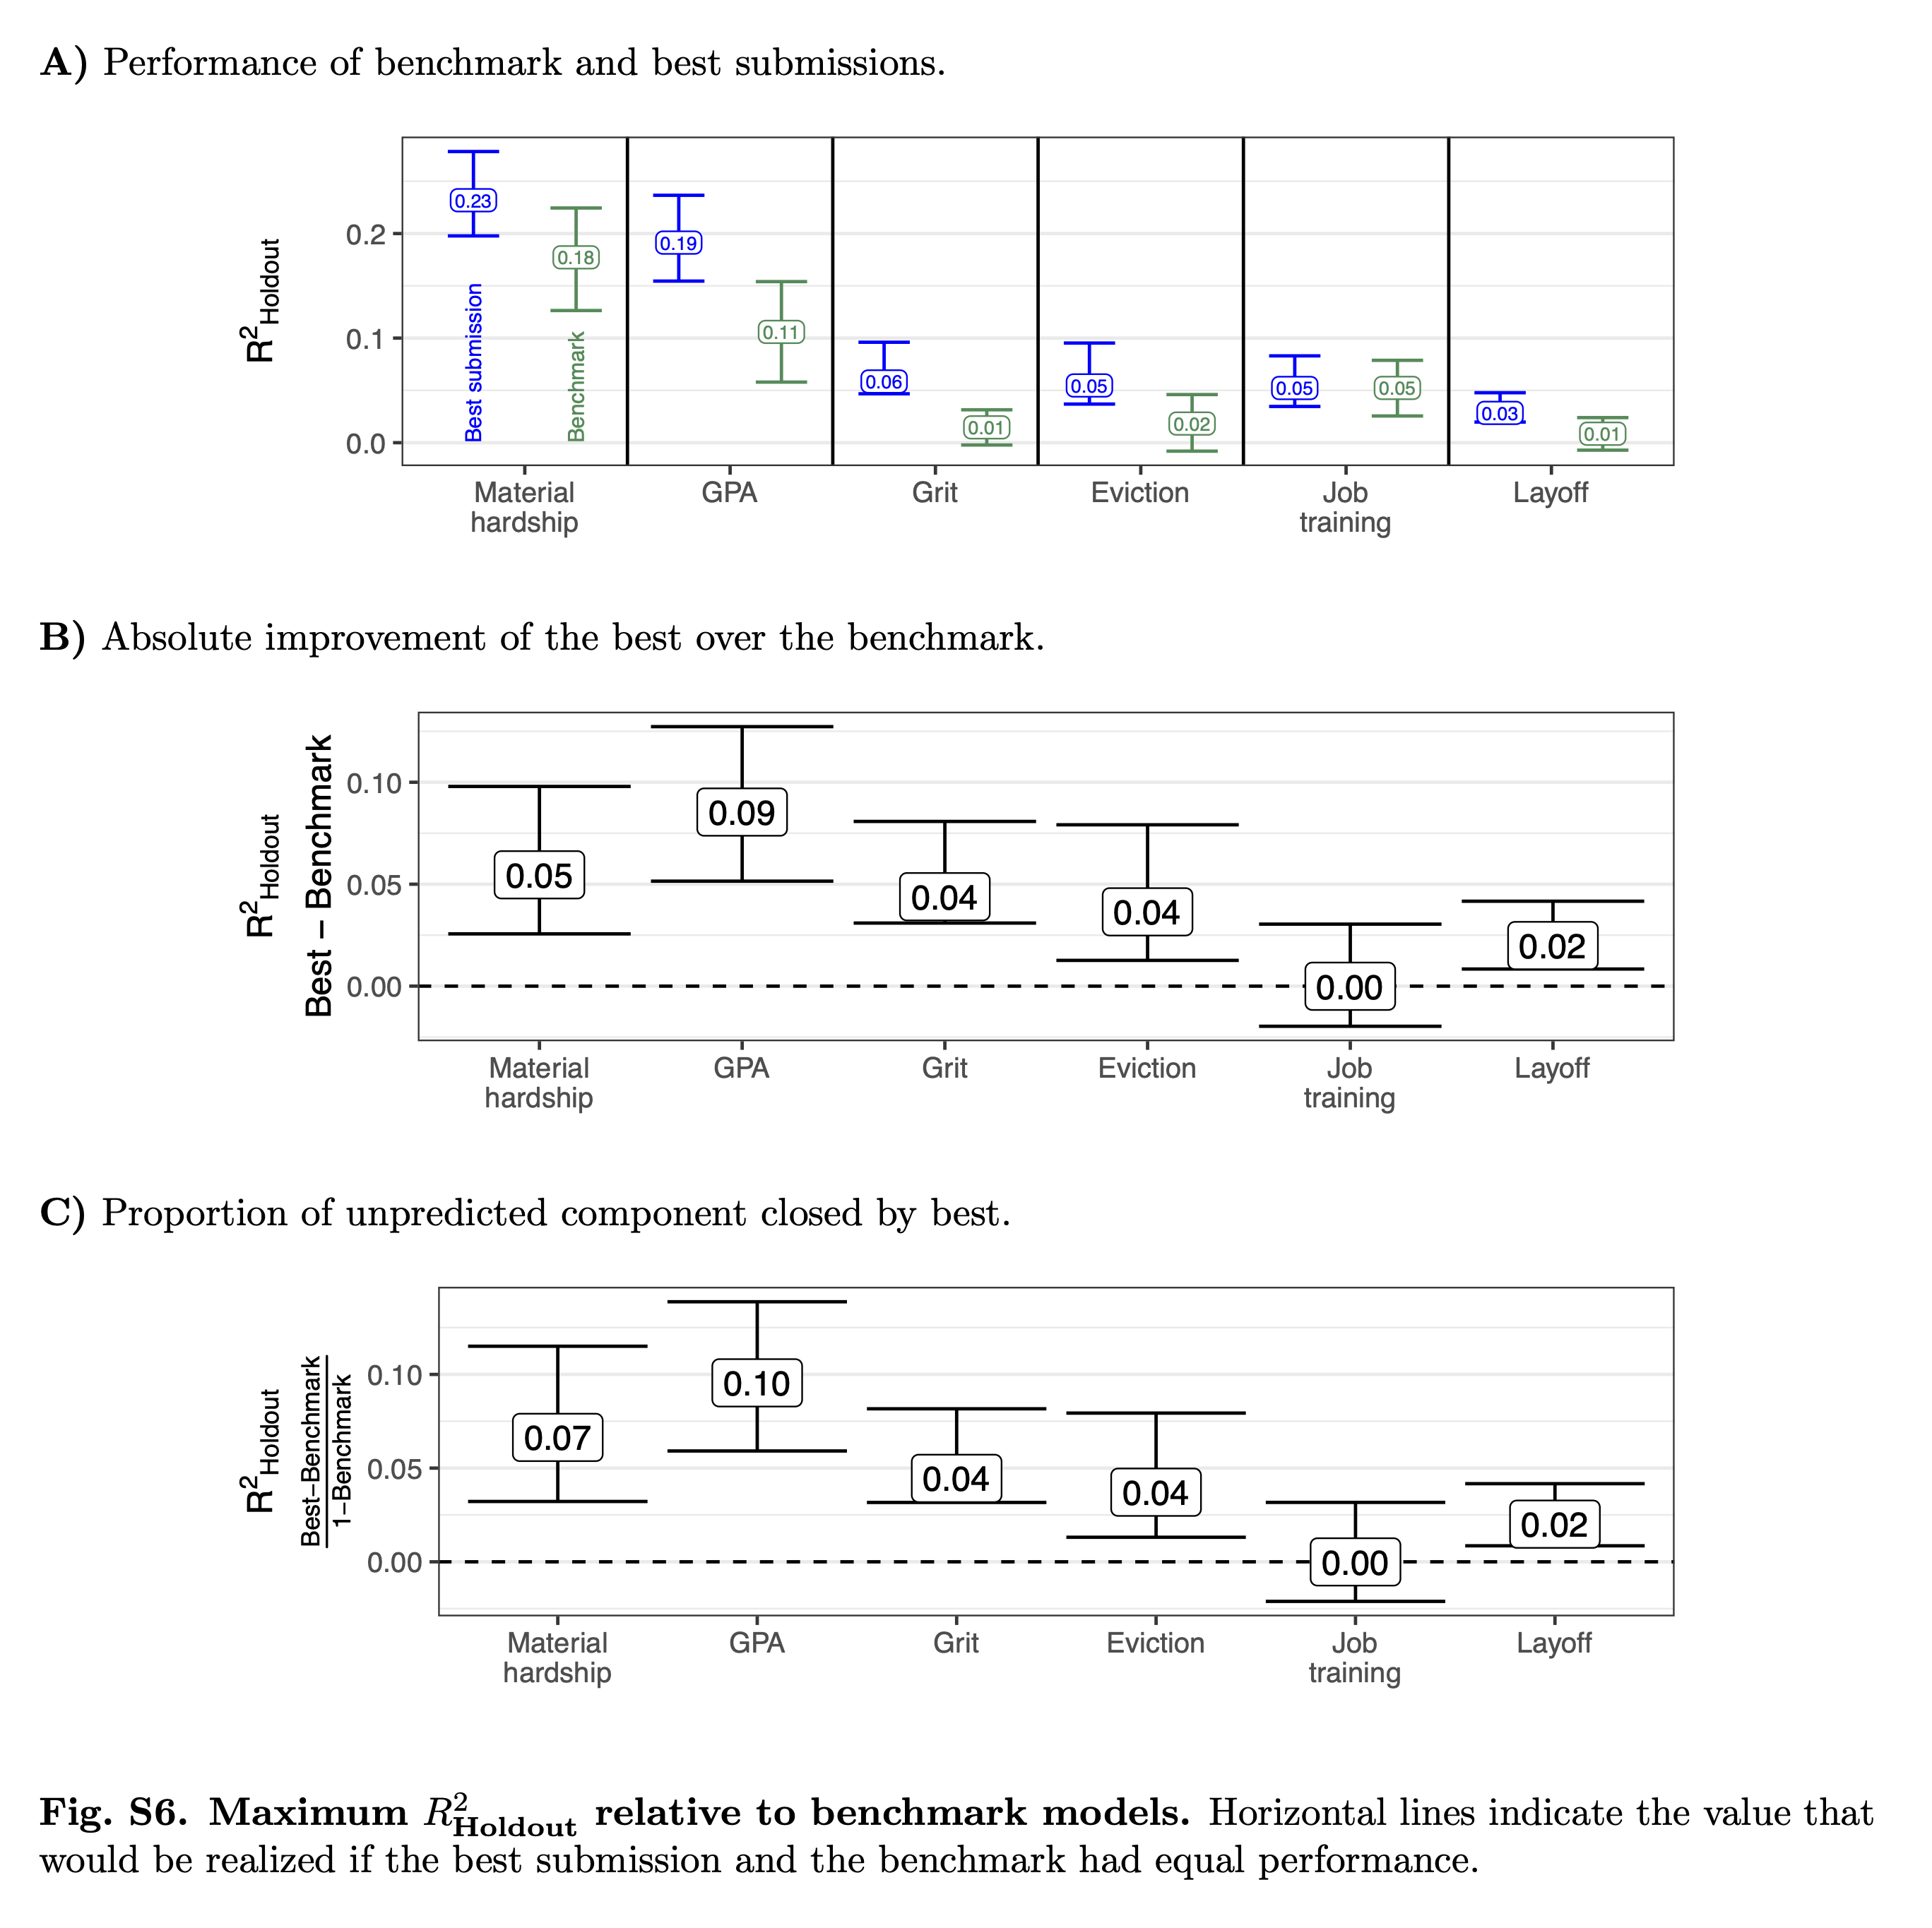
\includegraphics[height = .8\textheight]{figures/si_best_vs_benchmark}
\end{frame}

\begin{frame}{Appendix}
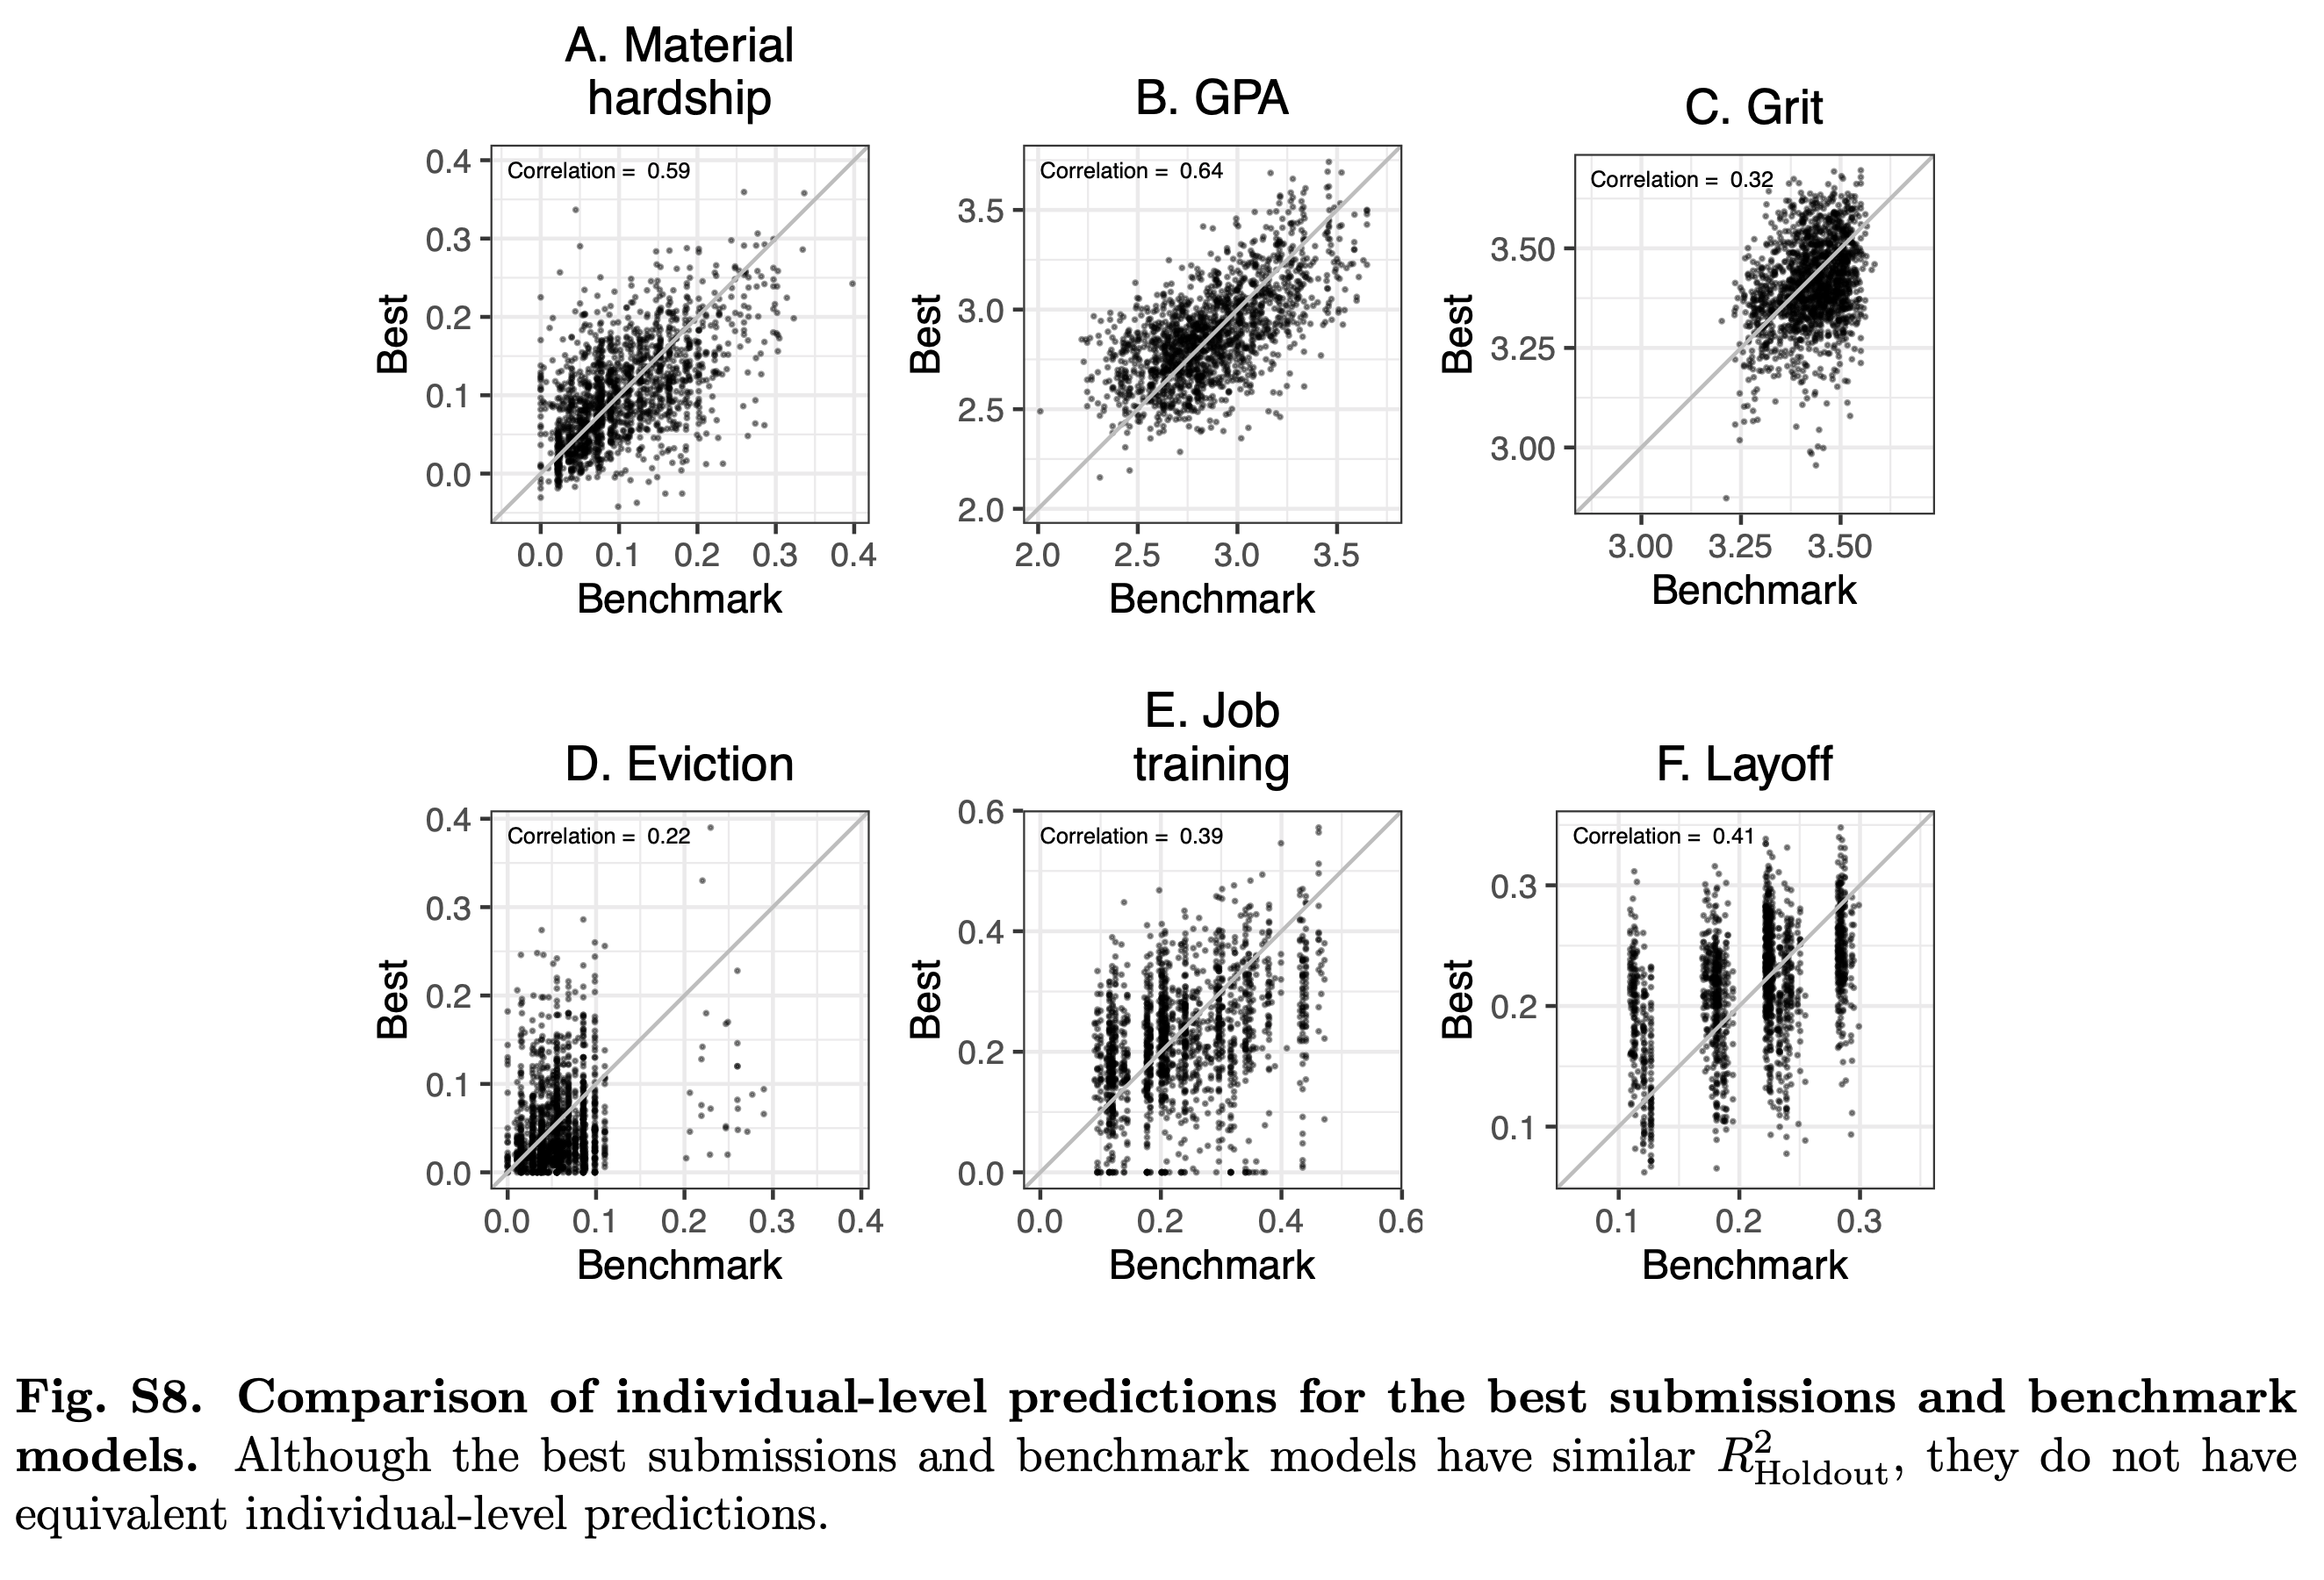
\includegraphics[width = \textwidth]{figures/si_best_benchmark_scatter}
\end{frame}

\begin{frame}{Appendix}
\includegraphics[width = \textwidth]{figures/si_worse_than_benchmark}
\end{frame}

\begin{frame}{Appendix}
\includegraphics[width = \textwidth]{figures/si_ensemble}
\end{frame}

\begin{frame}{Appendix}
\includegraphics[width = \textwidth]{figures/si_best_teams}
\end{frame}

\begin{frame}{Appendix}
\includegraphics[width = \textwidth]{figures/si_algorithms}
\end{frame}


\end{document}

